%**************************************************************************************
% License:
% CC BY-NC-SA 4.0 (http://creativecommons.org/licenses/by-nc-sa/4.0/)
%**************************************************************************************

\documentclass[notes]{beamer}

\mode<presentation> {

\usetheme{Madrid}

% Burnt orange
\definecolor{burntorange}{rgb}{0.8, 0.33, 0.0}
\colorlet{beamer@blendedblue}{burntorange}
% Pale yellow
\definecolor{paleyellow}{rgb}{1.0, 1.0, 0.953}
\setbeamercolor{background canvas}{bg=paleyellow}
% Secondary and tertiary palett
\setbeamercolor*{palette secondary}{use=structure,fg=white,bg=burntorange!80!black}
\setbeamercolor*{palette tertiary}{use=structure,fg=white,bg=burntorange!60!black}

% To remove the footer line in all slides uncomment this line
%\setbeamertemplate{footline}
% To replace the footer line in all slides with a simple slide count uncomment this line
%\setbeamertemplate{footline}[page number]

% To remove the navigation symbols from the bottom of all slides uncomment this line
%\setbeamertemplate{navigation symbols}{}
}

\usepackage{amsmath}
\usepackage{bm}
\usepackage{breqn}
\usepackage{graphicx} % for figures
\usepackage{subcaption} % for subplots 
\usepackage[labelsep=space,tableposition=top]{caption}
\renewcommand{\figurename}{Fig.} 
\usepackage{cleveref}
\usepackage{caption,subcaption}% http://ctan.org/pkg/{caption,subcaption}
\usepackage{booktabs} % Allows the use of \toprule, \midrule and \bottomrule in tables
\usepackage{multirow}

% To print 2 slides on a page
%\usepackage{handoutWithNotes}
%\pgfpagesuselayout{2 on 1}[border shrink=2mm]
%----------------------------------------------------------------------------------------
%	TITLE PAGE
%----------------------------------------------------------------------------------------
% The short title appears at the bottom of every slide, the full title is only on the title page
\title[CE394M: FEM Geo - case-study]{CE394M: Nicoll Highway Collapse: A case-study} 
\author{Krishna Kumar} % name
\institute[UT Austin] % institution 
{
University of Texas at Austin \\
\medskip
\textit{
  \url{krishnak@utexas.edu}} % Your email address
}
\date{\today} % Date, can be changed to a custom date

\begin{document}

\begin{frame}
\titlepage % title page as the first slide
\end{frame}

\begin{frame}
 % Table of contents slide, comment this block out to remove it
 \frametitle{Overview}
  %Throughout your presentation, if you choose to use \section{} and \subsection{} 
  %commands, these %will automatically be printed on this slide as an overview 
 \tableofcontents
\end{frame}

%----------------------------------------------------------------------------------------
% slides
%----------------------------------------------------------------------------------------
\section{Geotechnical FEA}
%------------------------------------------------
\begin{frame}
\frametitle{FE Disclaimer}
\begin{figure}[ht]
	\centering
	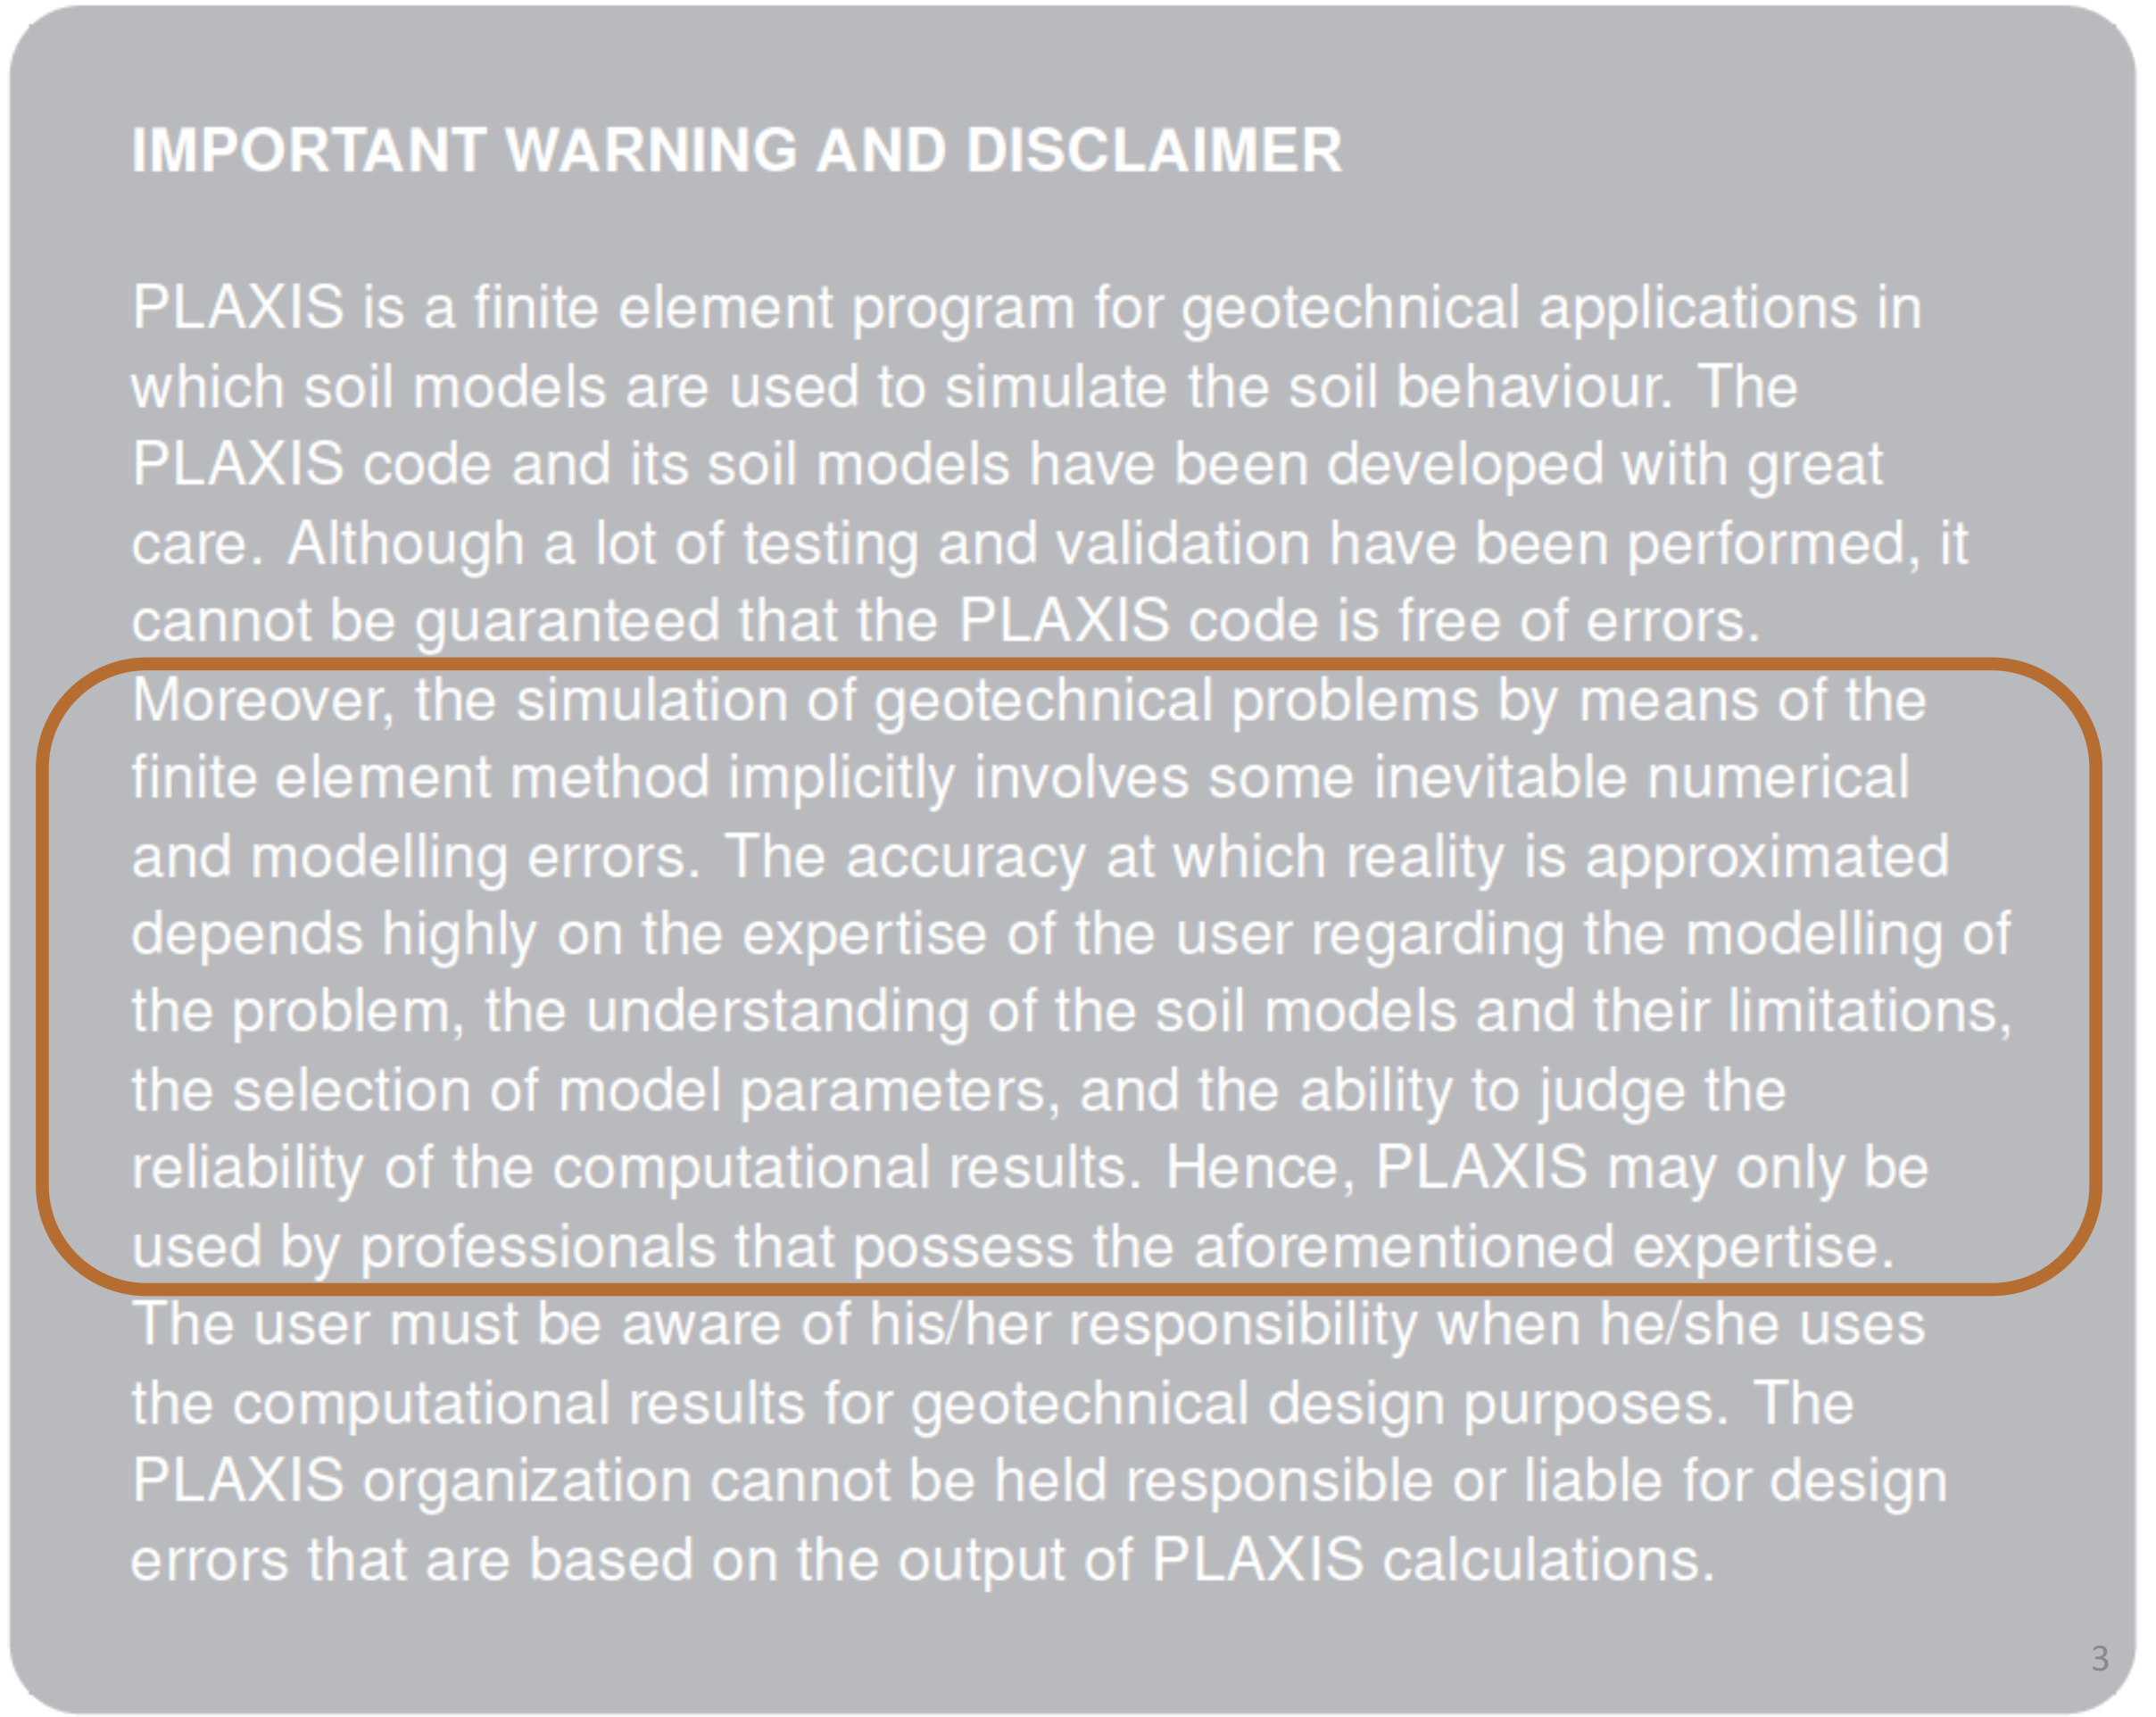
\includegraphics[width=0.85\textwidth]{figs/plaxis-disclaimer.png}
\end{figure}
\end{frame}

%------------------------------------------------
\begin{frame}
\frametitle{Consistent system of units}
\begin{figure}[ht]
	\centering
	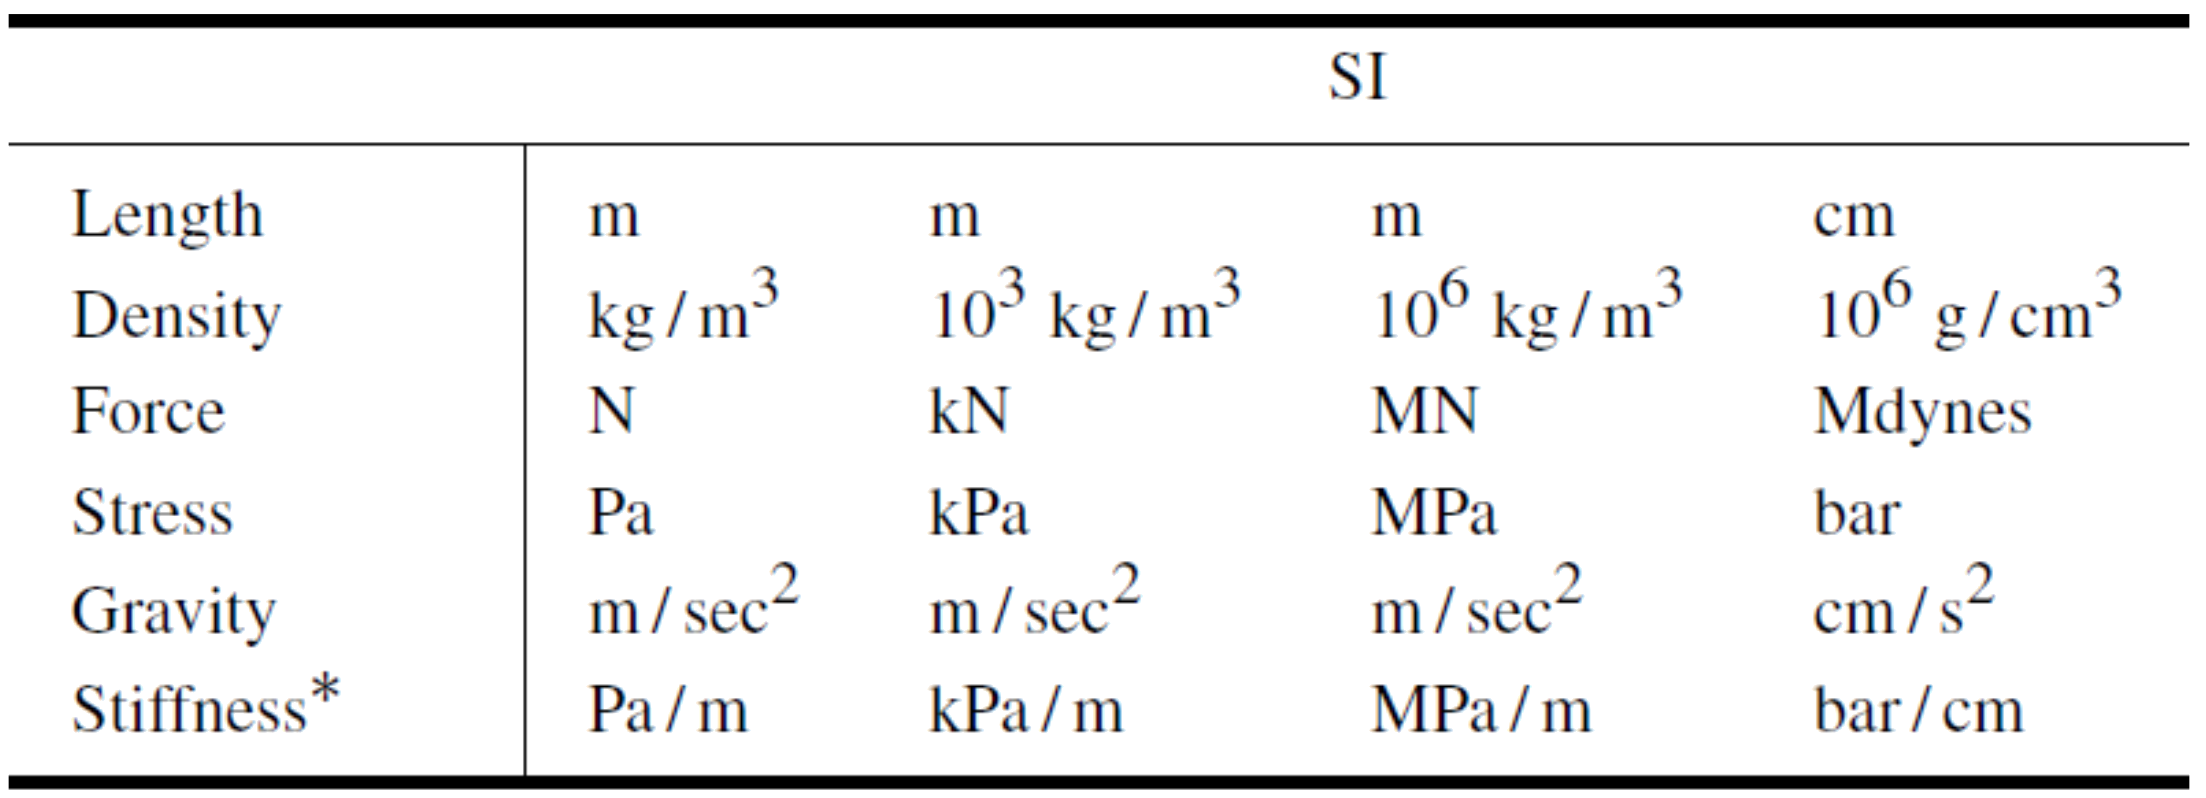
\includegraphics[width=0.85\textwidth]{figs/units.png}
\end{figure}
\end{frame}

%------------------------------------------------
\begin{frame}
\frametitle{Problem definition}
\mode<beamer>{
	\begin{figure}[ht]
		\centering
		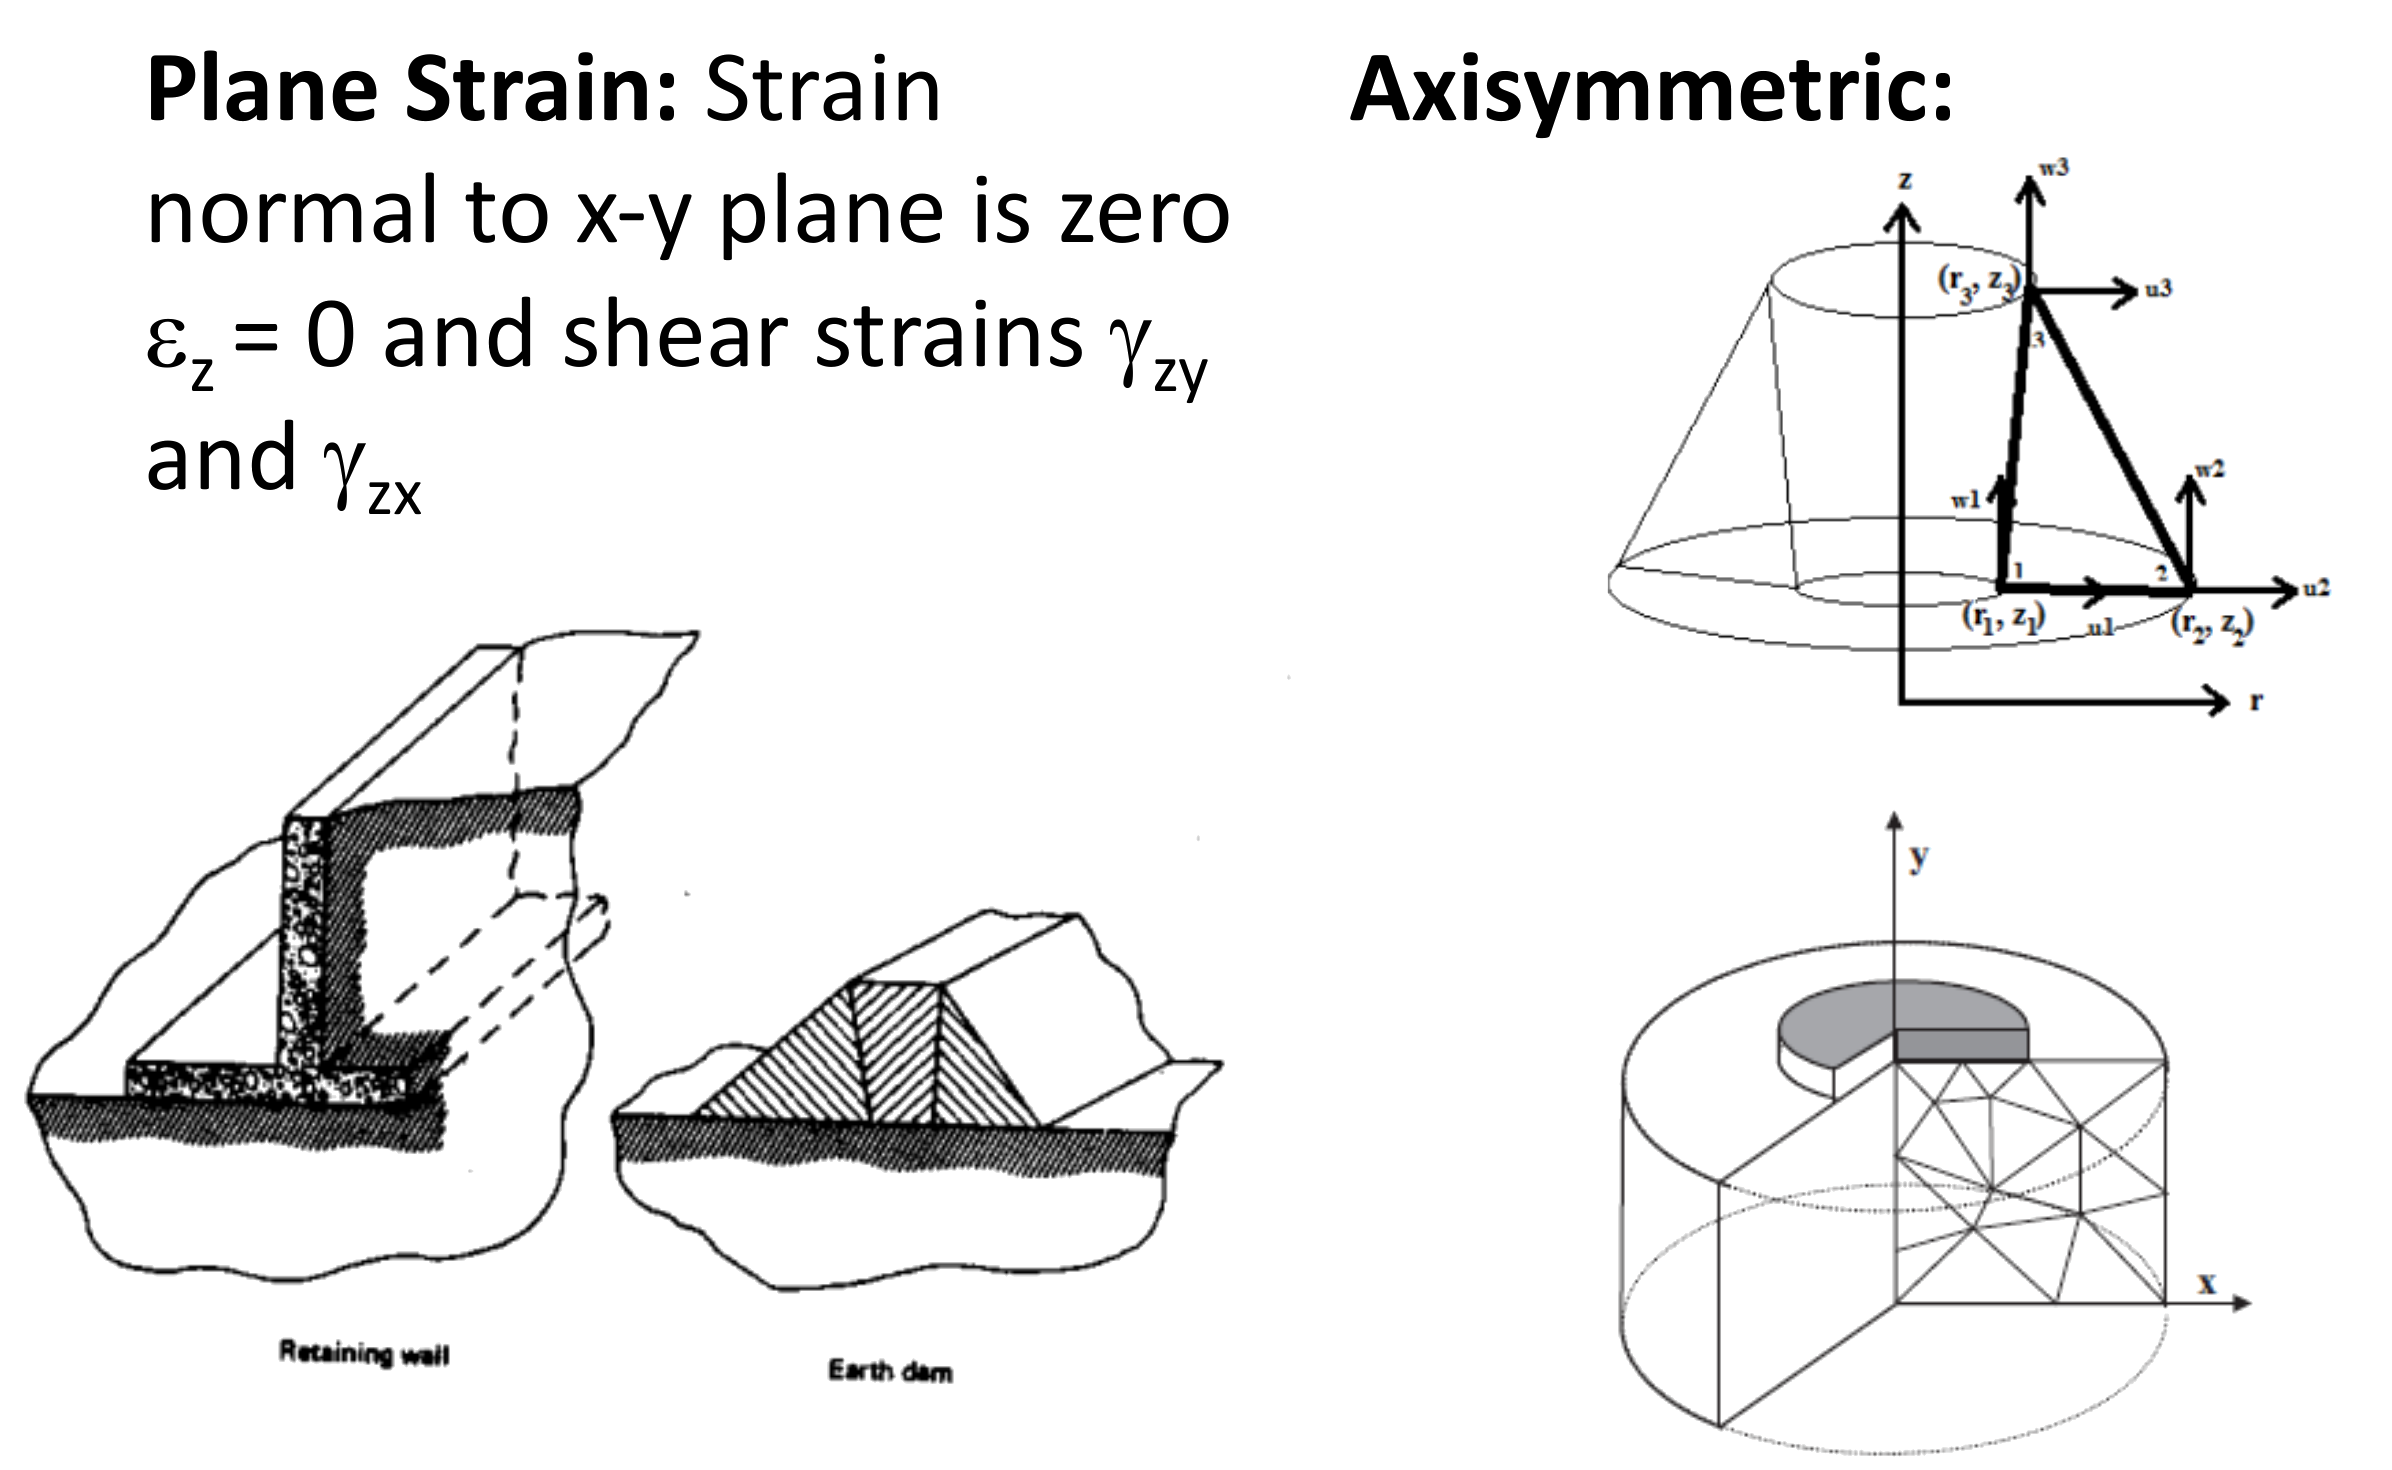
\includegraphics[width=0.85\textwidth]{figs/planestrain-axisymmetric.png}
		\caption*{Take advantage of symmetry}
	\end{figure}
}
\mode<handout>{
	\vspace{6cm}
}
\end{frame}

\note{
	\begin{figure}[ht]
		\centering
		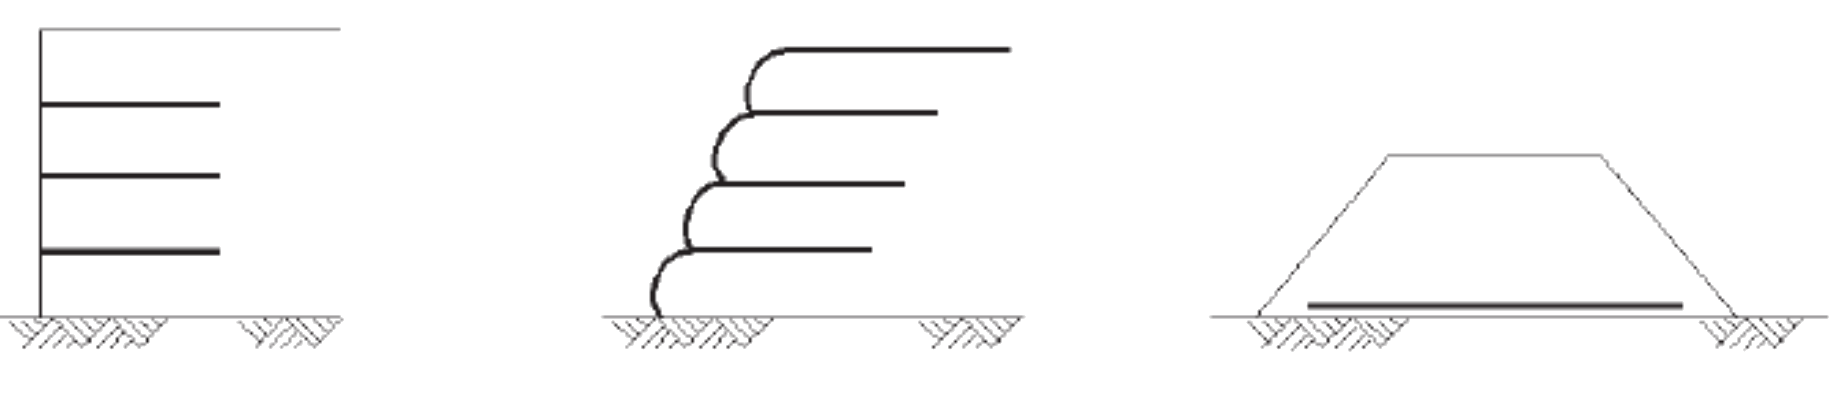
\includegraphics[width=0.85\textwidth]{figs/geogrids.png}
		\caption*{Take advantage of symmetry}
	\end{figure}
}

\subsection{Element types}
%------------------------------------------------
\begin{frame}
\frametitle{1D Finite Elements: Bar element}
Two node element with axial stiffness only (no flexural or shear
resistance).\mode<beamer>{Examples of this type of structure are cables, reinforcing bars.}
\begin{figure}[ht]
	\centering
	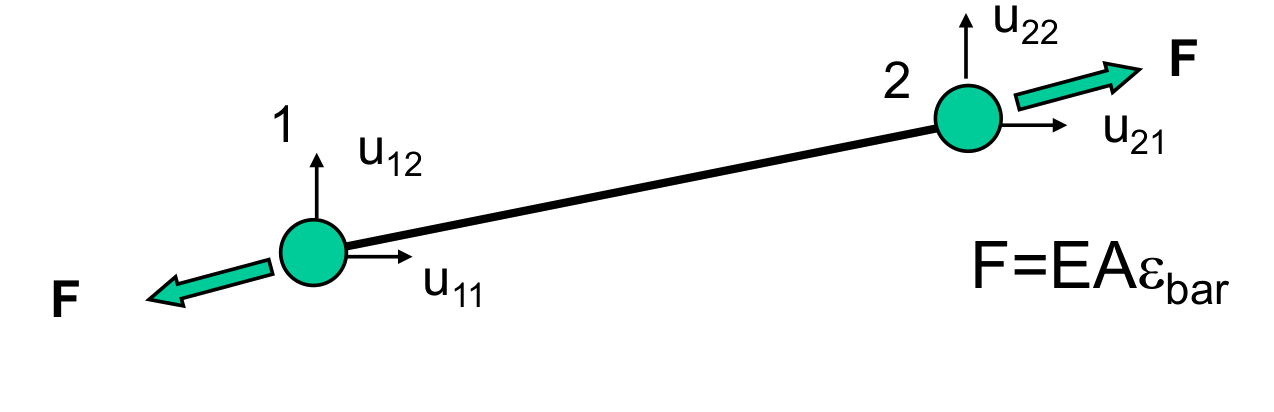
\includegraphics[width=0.65\textwidth]{figs/bar-element.png}
\end{figure}
\mode<handout>{
	\vspace{3cm}
}
\end{frame}

\note{
	\begin{enumerate}
		\item Node to Node: are sprints that are used to model ties between two points. 
		\item It’s not recommended to draw geometry line at position where node-to-node anchor is to be placed. 
		\item It’s a 2 node elastic spring element with normal stiffness (Spring constant)
		\item Element can sustain both tensile forces (anchors) as well as compressive forces (struts).
		\item Fixed-End anchors:  Modelling of struts or props to sheet pile walls. 
	\end{enumerate}
}

\note{
	\begin{enumerate}
		\item Geogrids are slender structures with a normal stiffness but no bending stifness. 
		\item Geogrids can only sustain \textbf{Tensile forces} and no compression!
		\item Structures involving geotextiles. 
	\end{enumerate}
	\begin{figure}[ht]
		\centering
		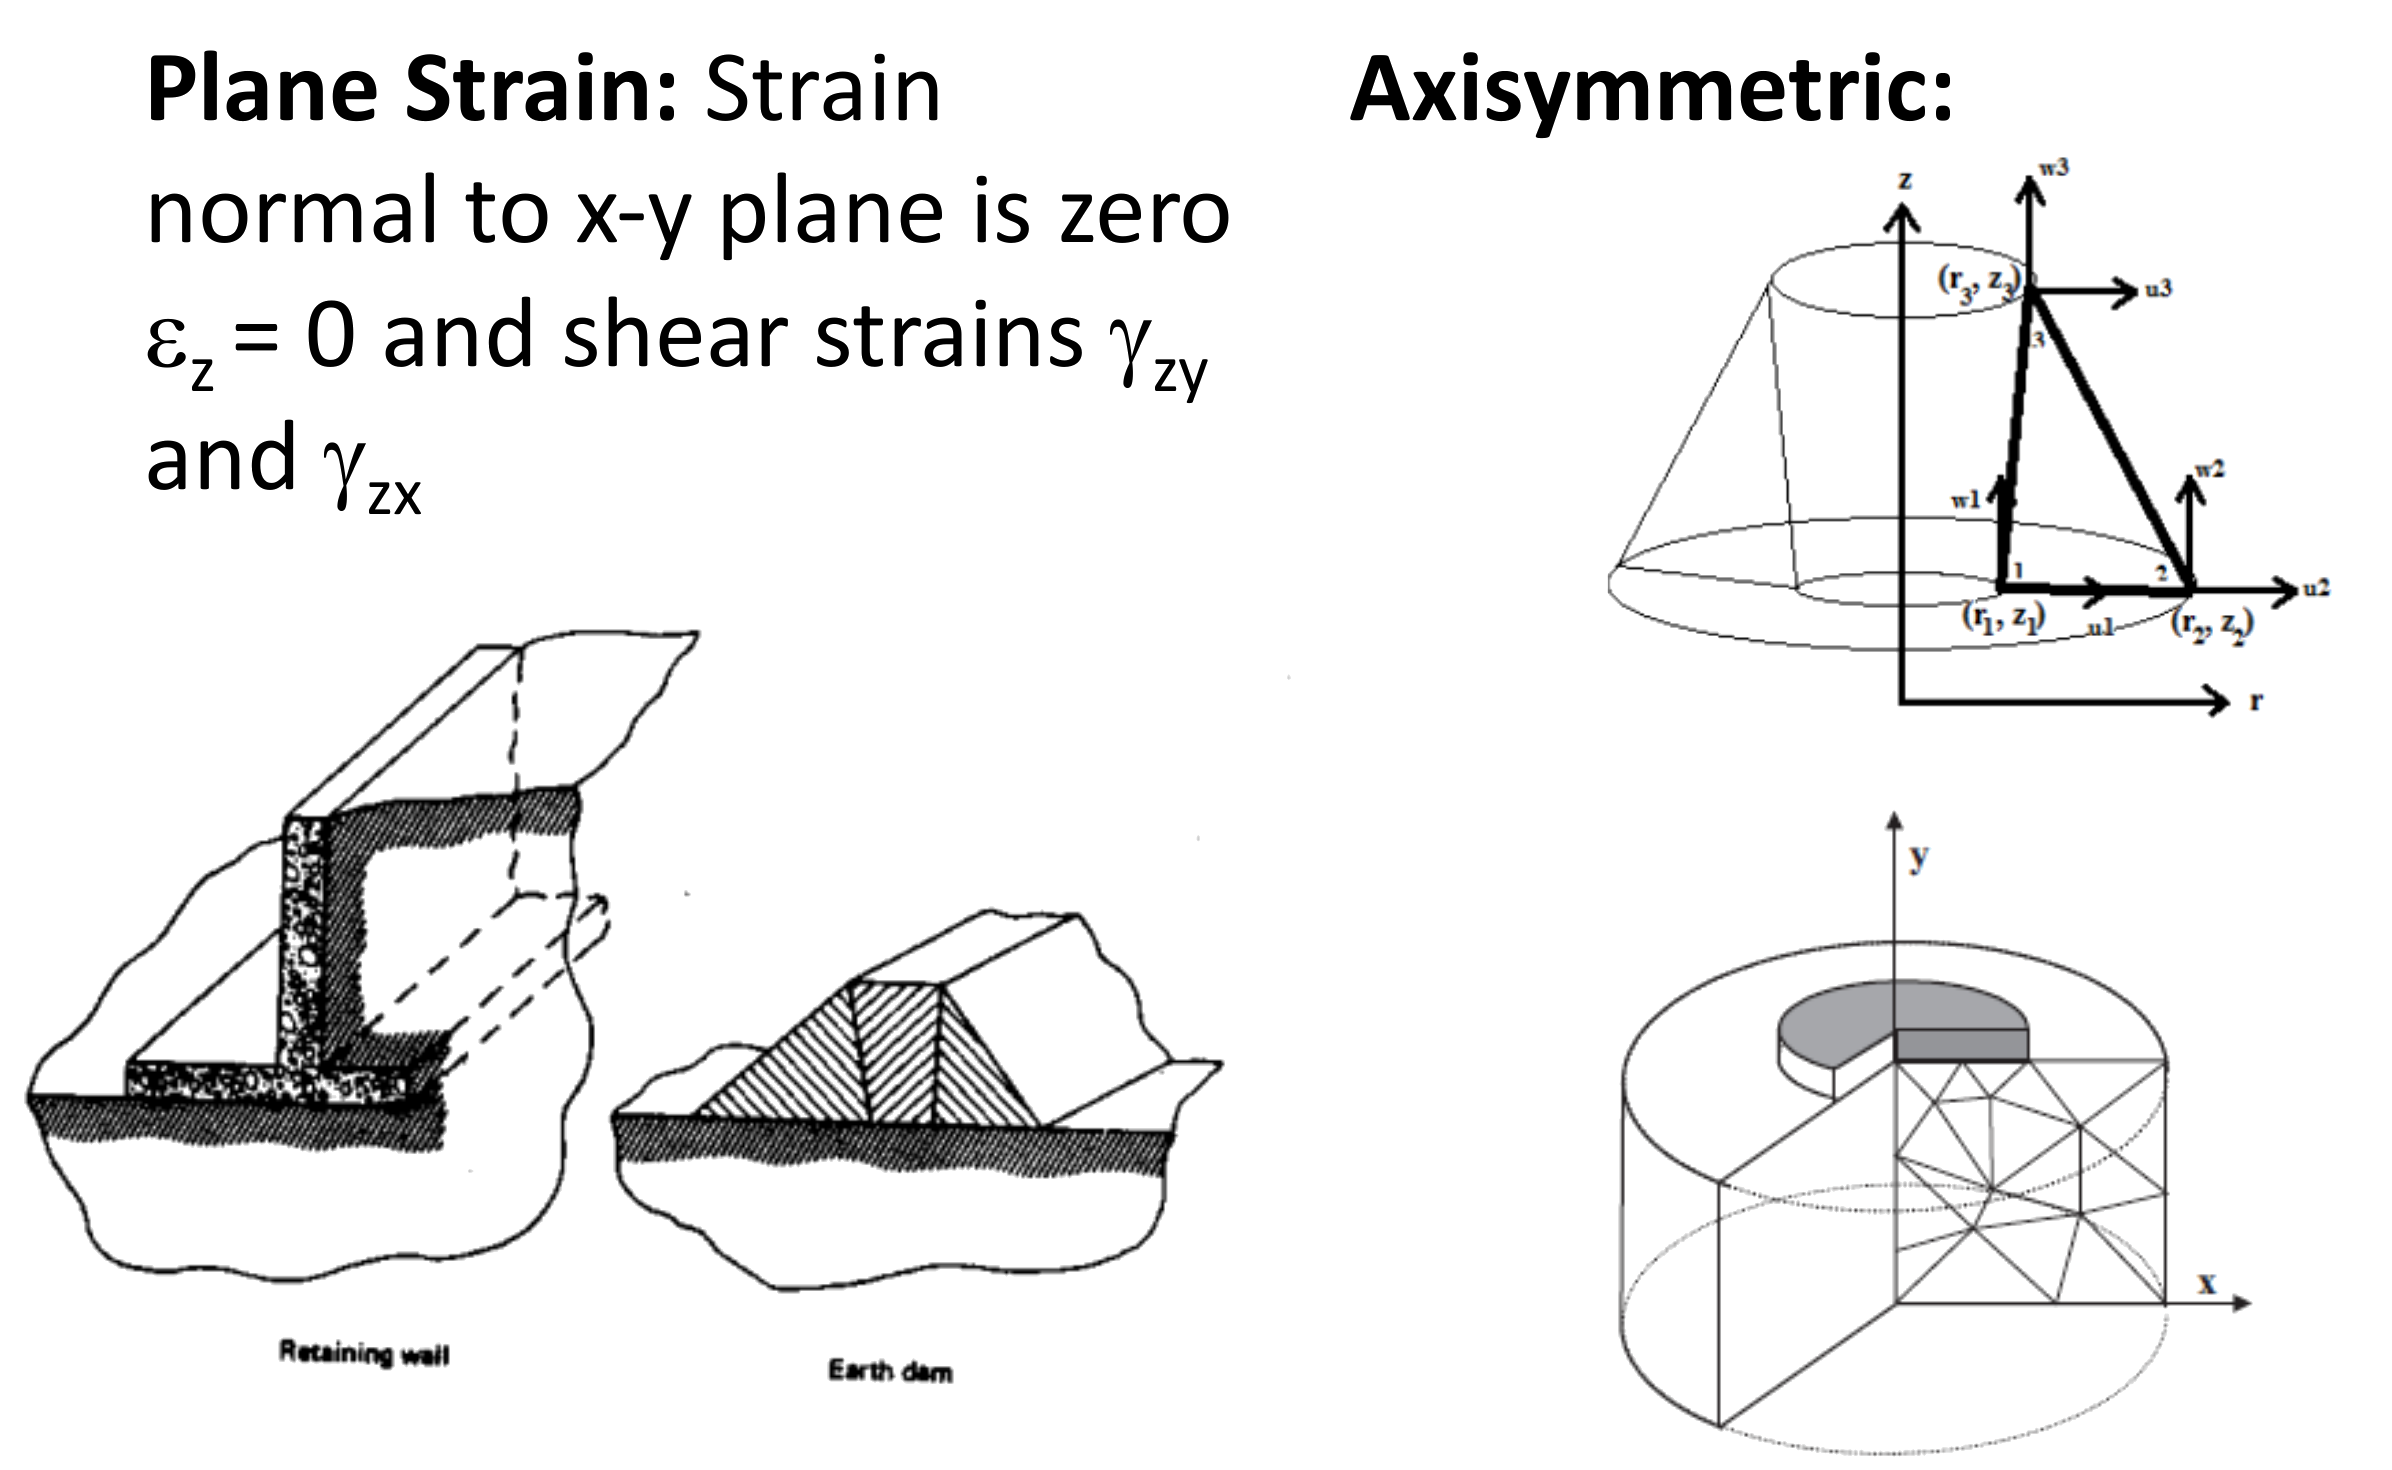
\includegraphics[width=0.85\textwidth]{figs/planestrain-axisymmetric.png}
		\caption{Take advantage of symmetry}
	\end{figure}
}

%------------------------------------------------
\begin{frame}
\frametitle{1D Finite Elements: Beam element}
two node structure element with axial and bending stiffness (no
transverse shear deformation). Three degrees of freedom for 2D beam element (1, 2
displacements and a moment)\mode<beamer>{Examples are sheet pile walls, structural foundation
	beams, structural facing for reinforced soil walls.}
\begin{figure}[h]
	\centering
	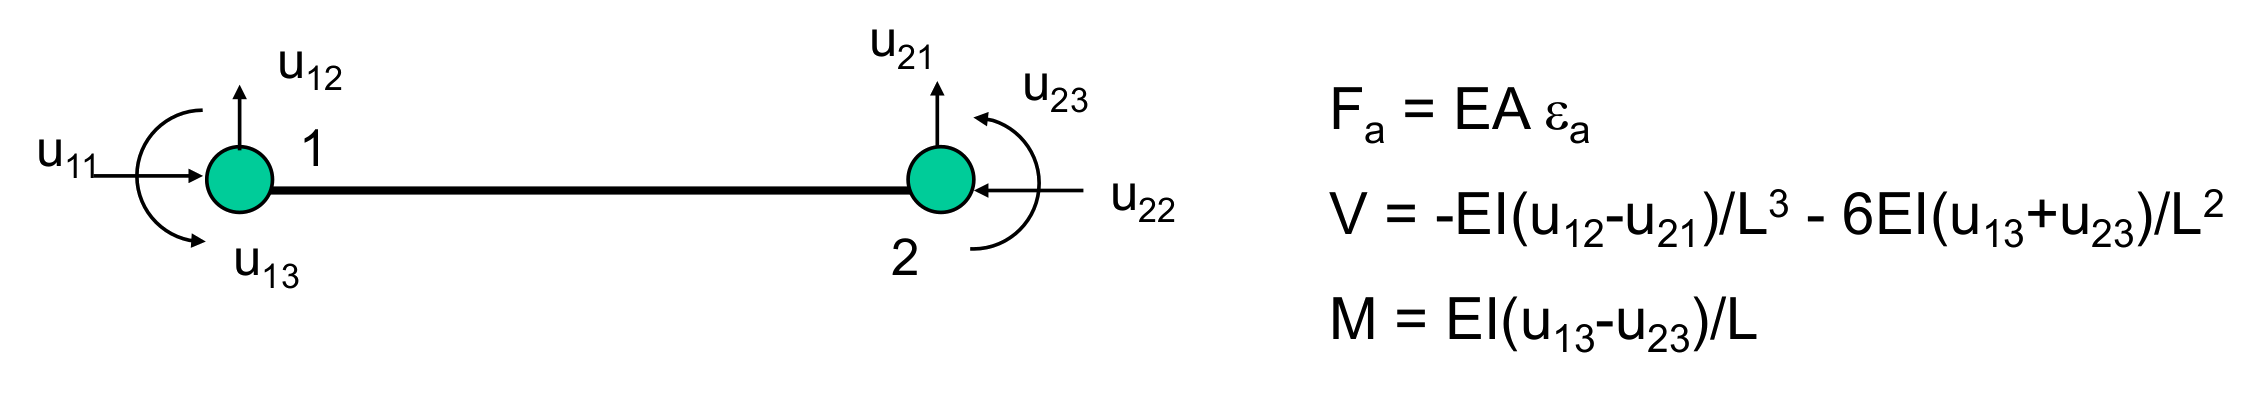
\includegraphics[width=0.75\textwidth]{figs/beam-element.png}
\end{figure}
\begin{figure}[h]
	\centering
	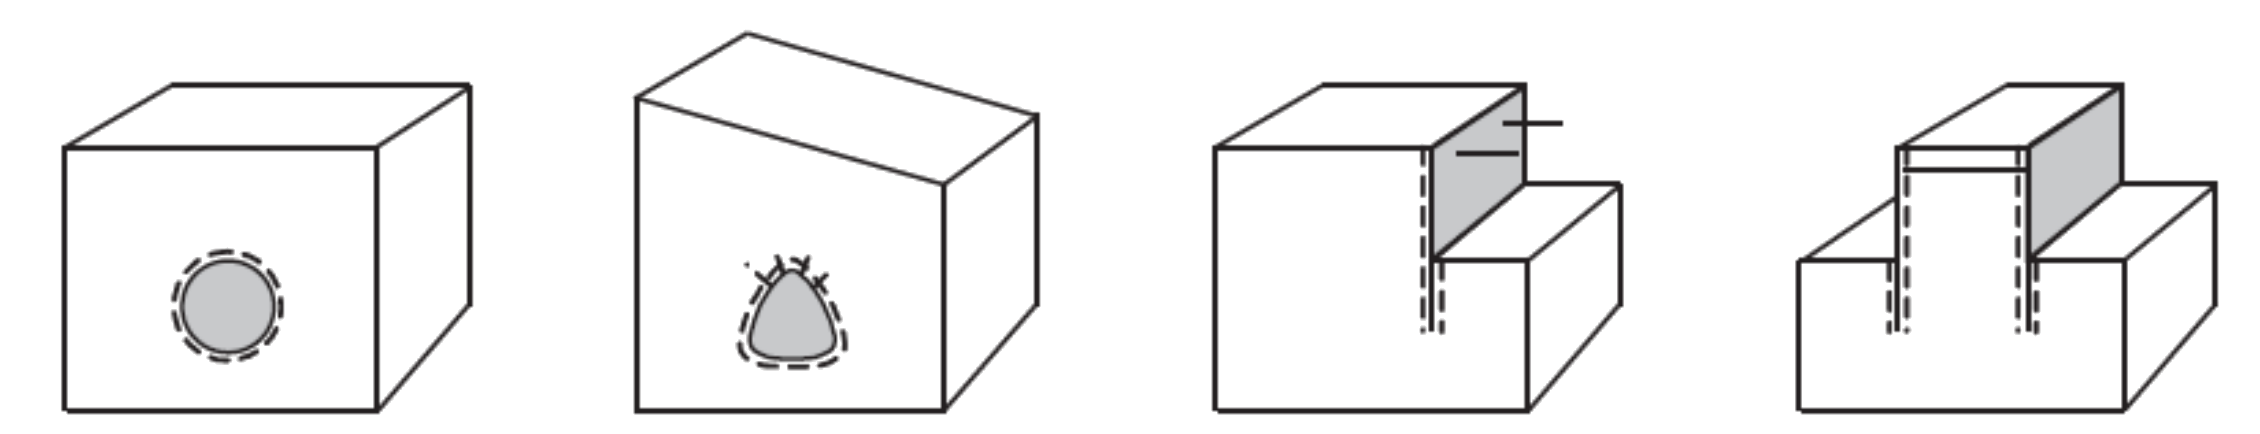
\includegraphics[width=0.75\textwidth]{figs/plate-elements.png}
\end{figure}
\end{frame}

%------------------------------------------------
\begin{frame}
\frametitle{2D plane-strain / axisymmetric elements}
\begin{figure}[ht]
	\centering
	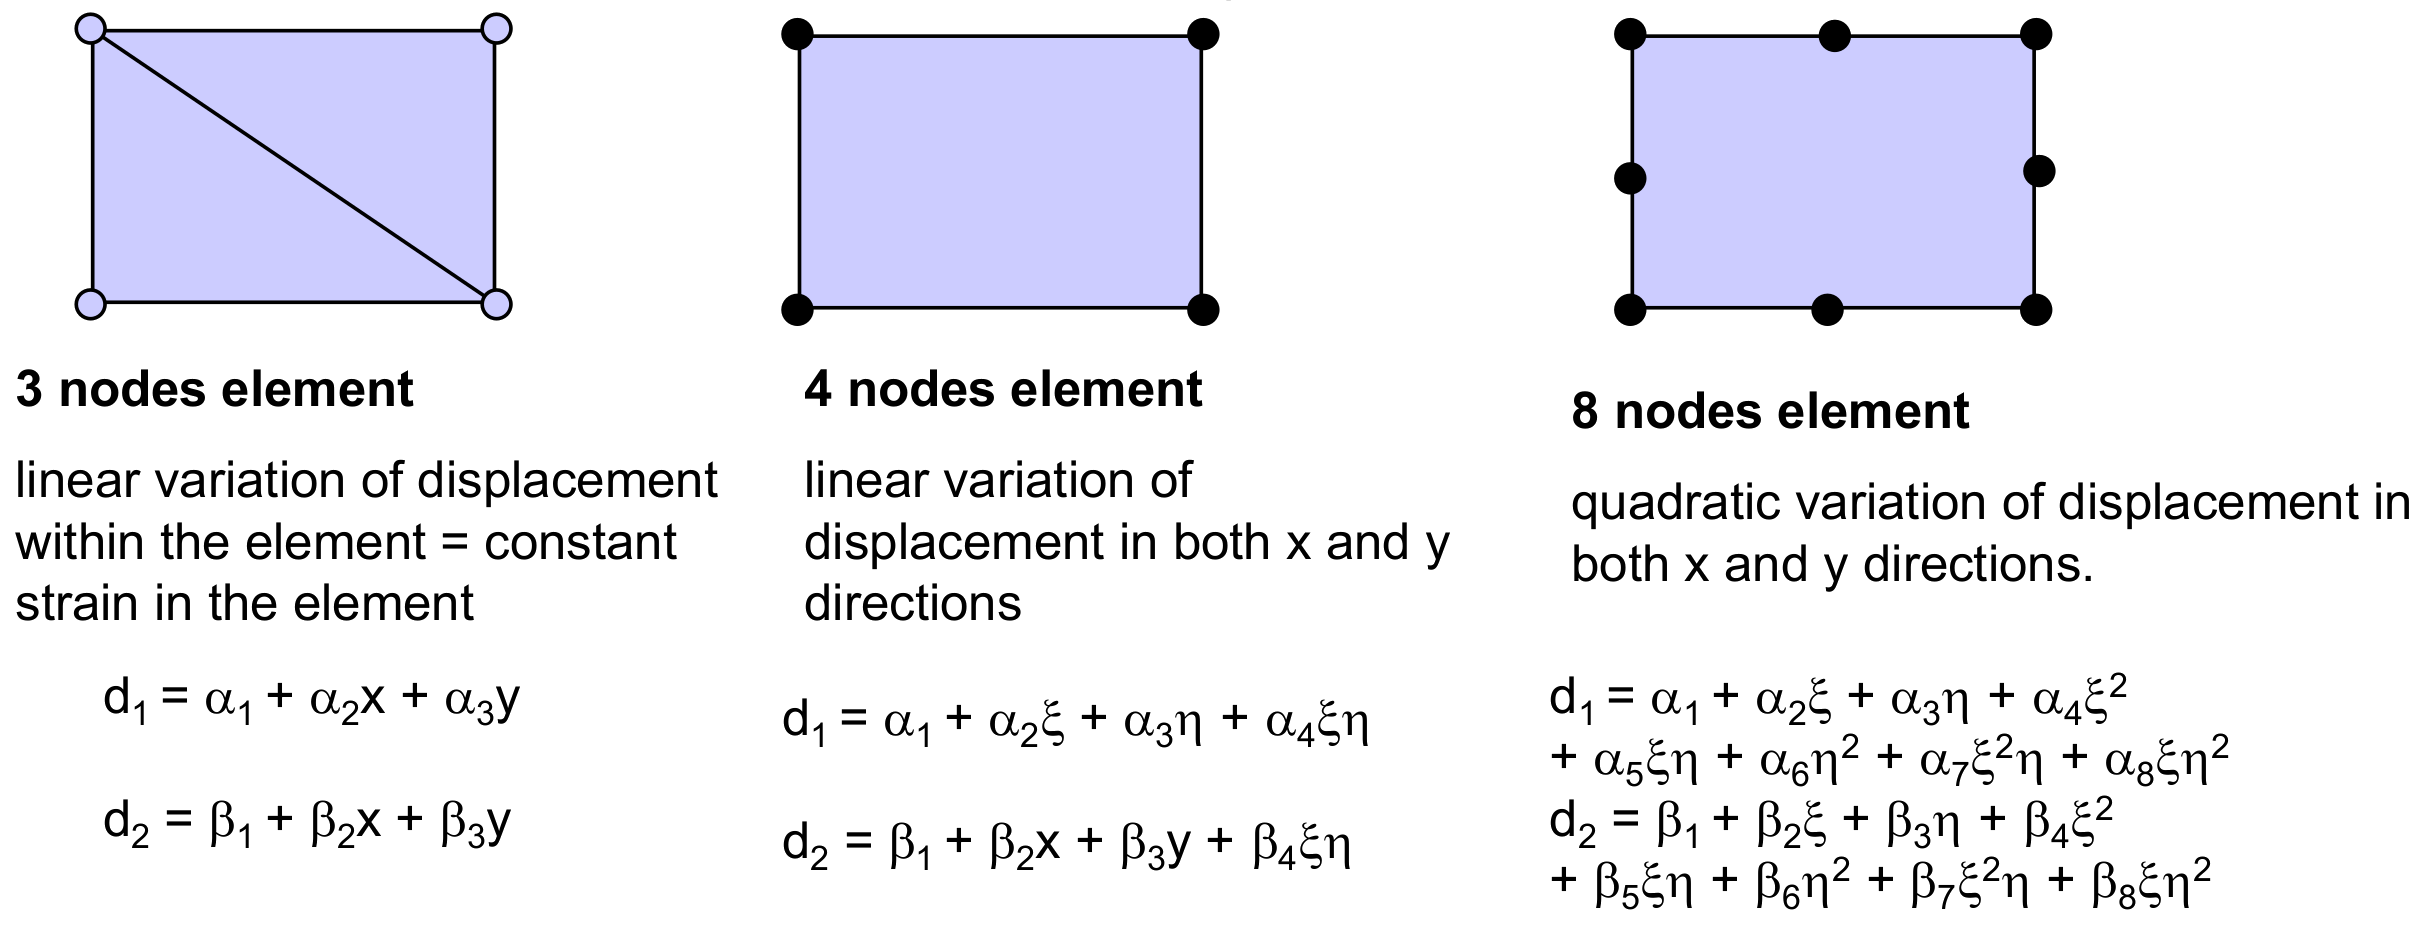
\includegraphics[width=\textwidth]{figs/2d-fe-elements.png}
\end{figure}
\end{frame}

%------------------------------------------------
\begin{frame}
\frametitle{2D/3D Finite elements}
\begin{figure}[ht]
	\centering
	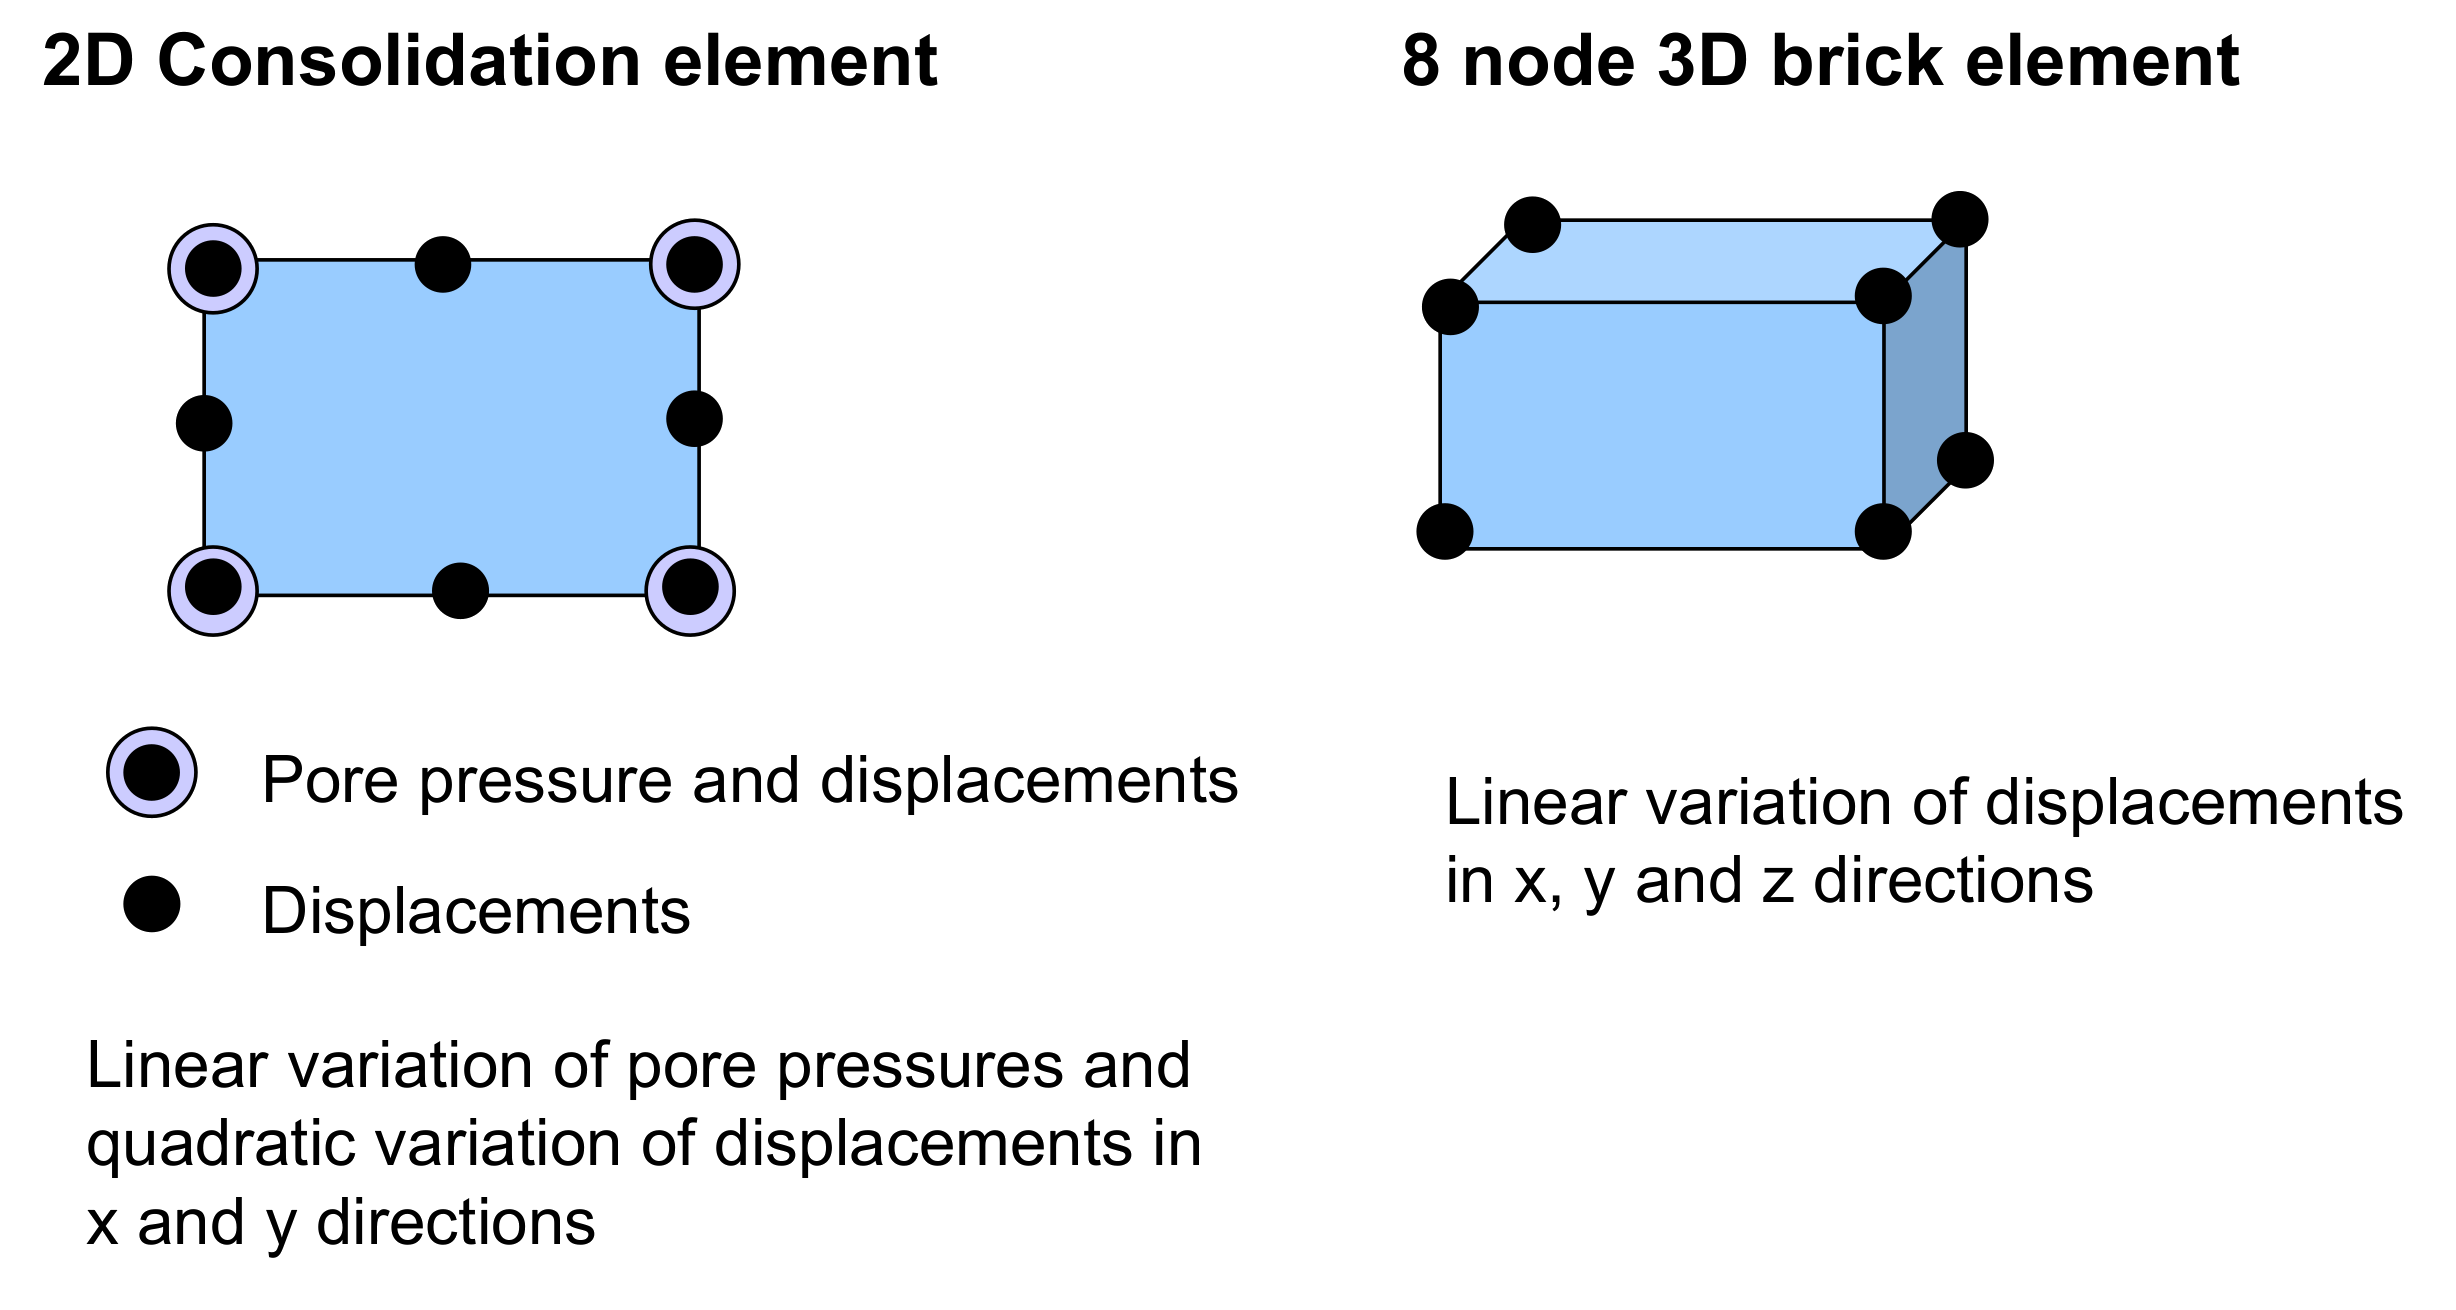
\includegraphics[width=\textwidth]{figs/2d-3d-elements.png}
\end{figure}
\end{frame}

%------------------------------------------------
\begin{frame}
\frametitle{Interface element}
\begin{figure}[ht]
	\centering
	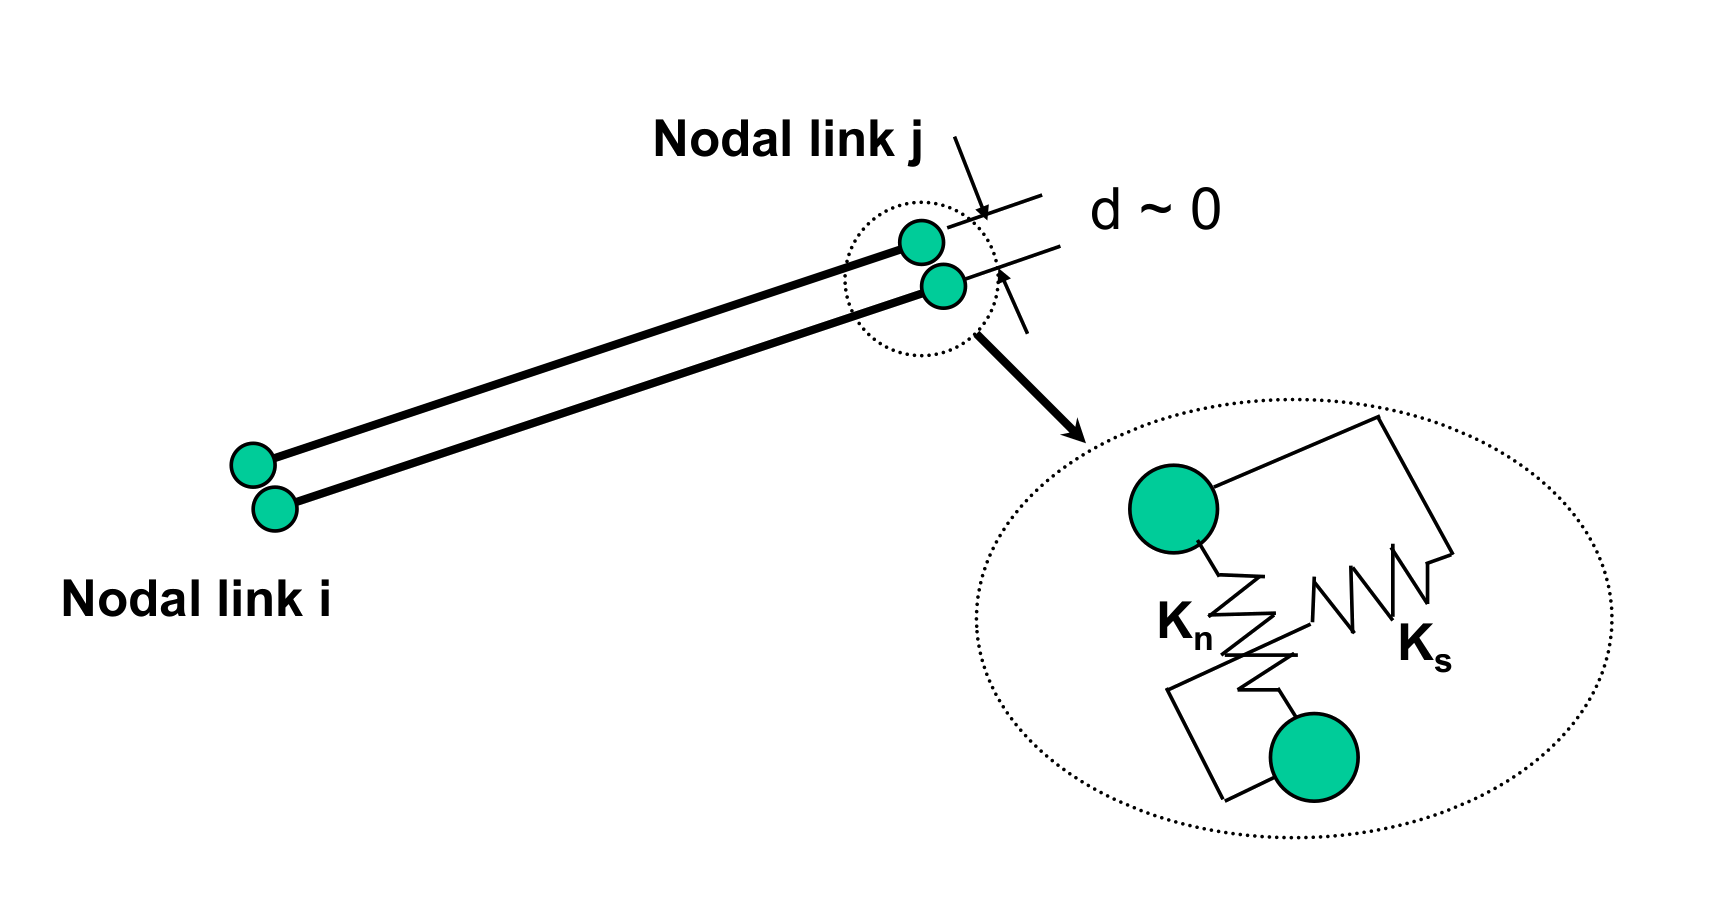
\includegraphics[width=0.5\textwidth]{figs/interface-element.png}
\end{figure}
\begin{figure}[ht]
	\centering
	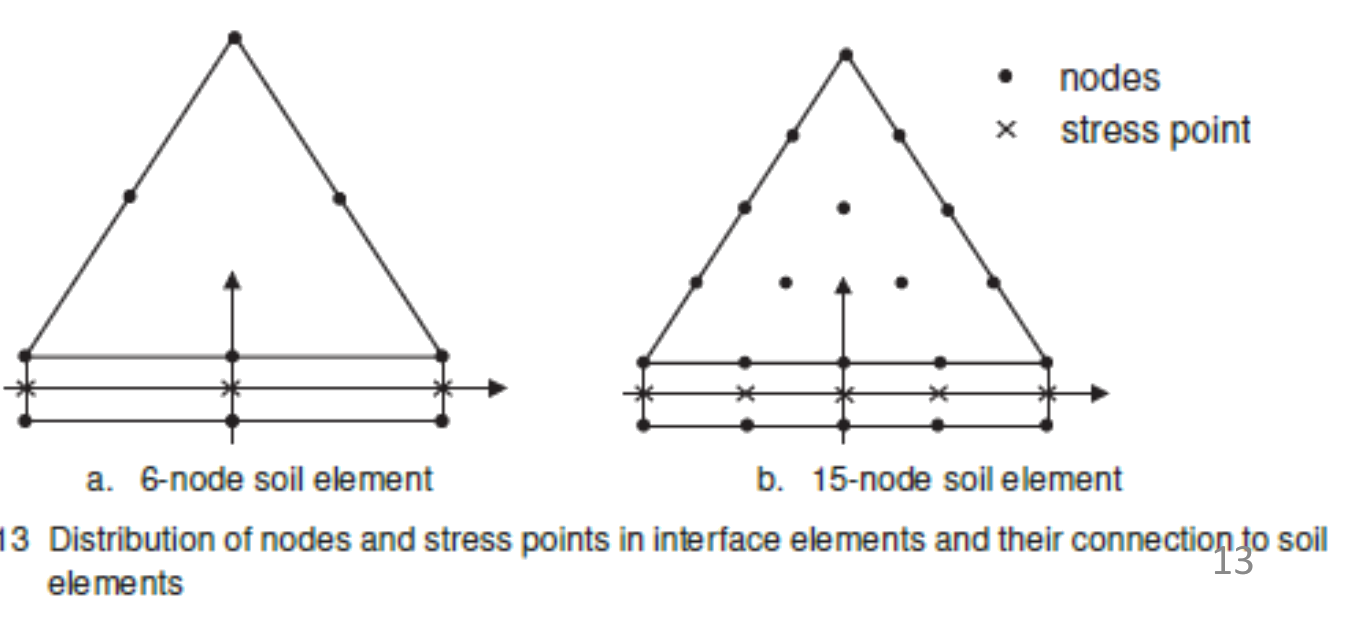
\includegraphics[width=0.6\textwidth]{figs/fe-interface.png}
	\caption*{Use a reduced strength at the interface}
\end{figure}
\end{frame}

\note{This element allows relative displacement between
elements. It is capable to model soil/structure interface conditions, shear planes
with in a soil mass. The element is ‘fictitious’ four node element made up of two
independent nodal links. Each link consists of two nodes connected by a normal
and shear spring as shown below. The stiffness of the springs can be non-linear,
modelling frictional slip behaviour. The thickness of the element is assumed to be
negligibles}

%------------------------------------------------
\begin{frame}
\frametitle{Interface elements for Soil Structure Interactions}
\begin{figure}[ht]
	\centering
	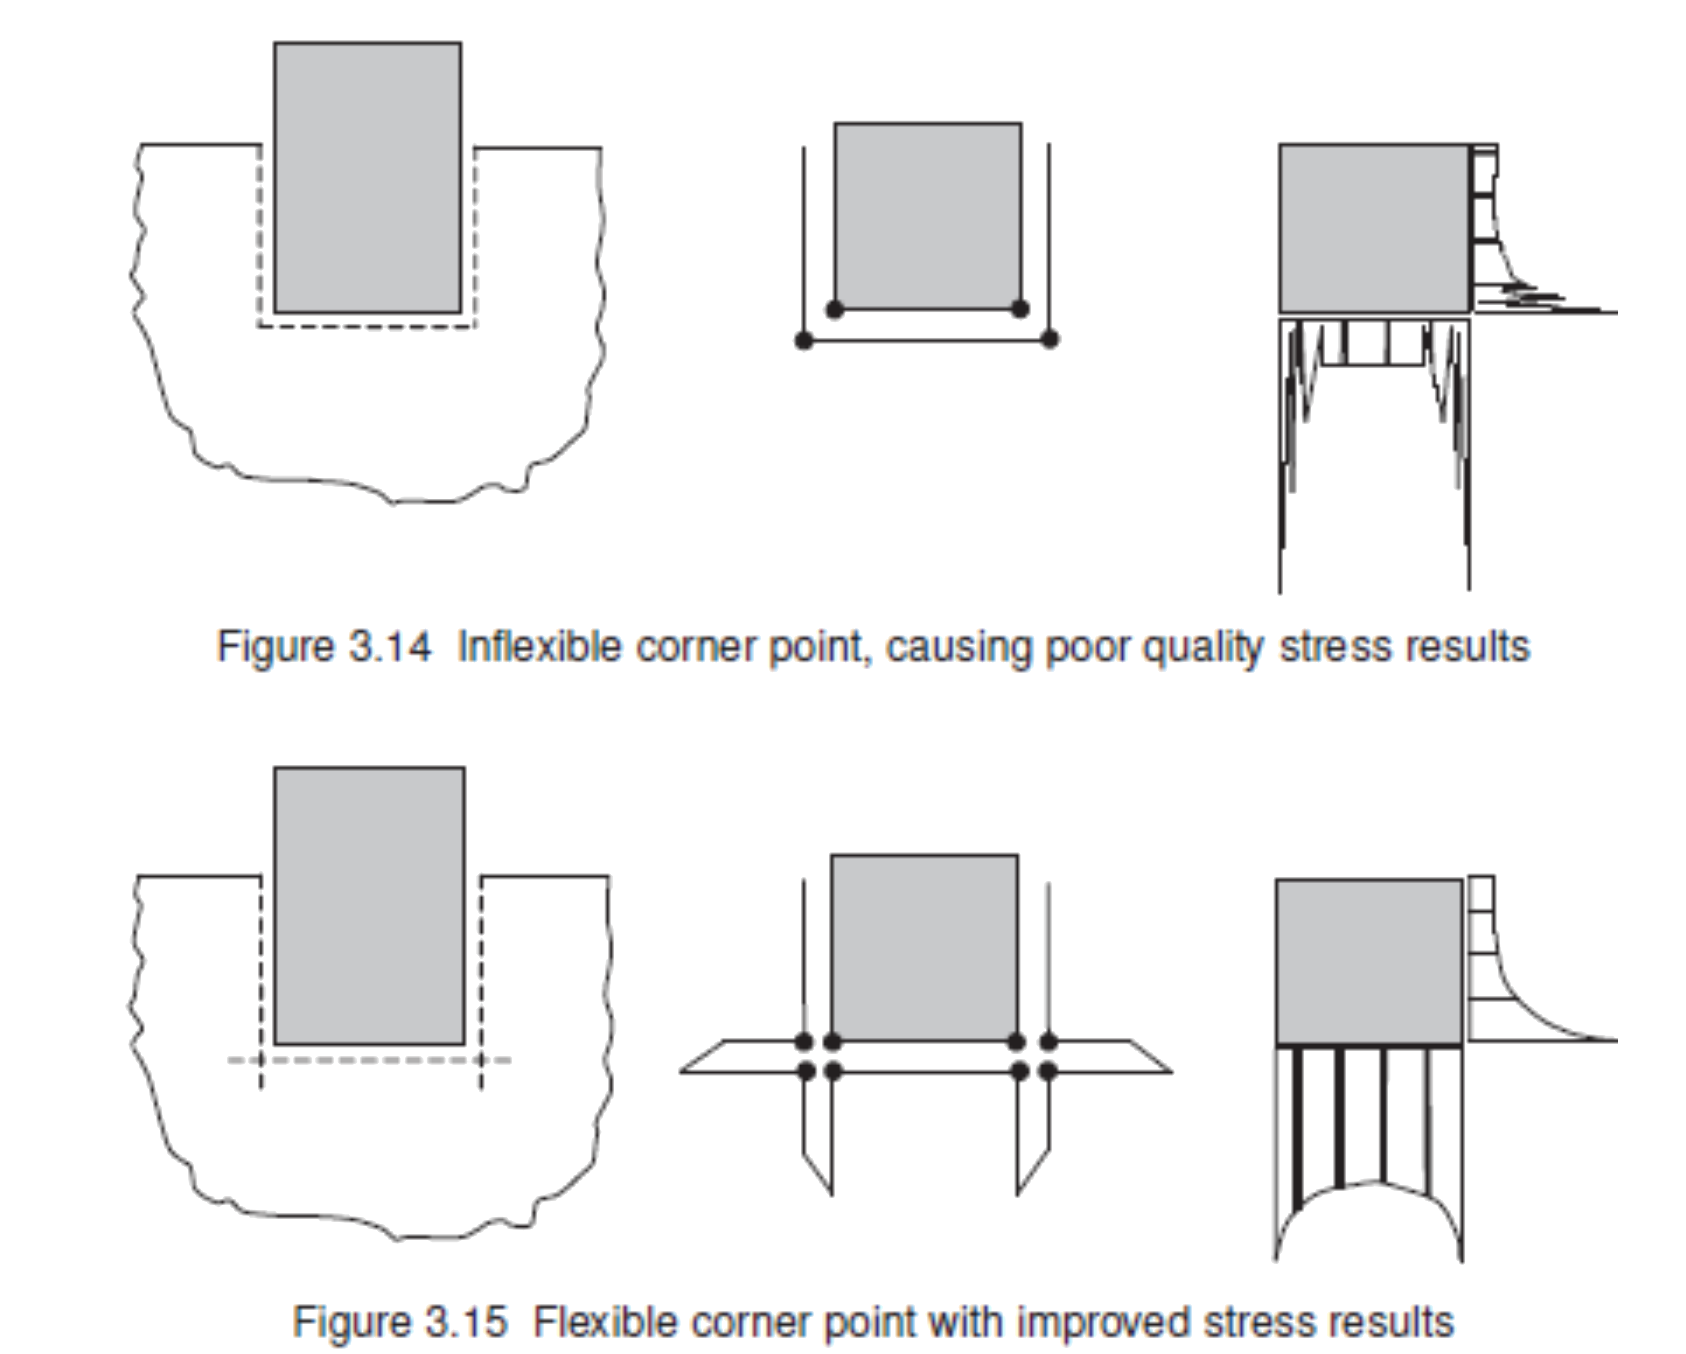
\includegraphics[width=0.65\textwidth]{figs/interface-ssi.png}
\end{figure}
\end{frame}

\subsection{Discretization}
%------------------------------------------------
\begin{frame}
\frametitle{FE discretization}
\begin{figure}[ht]
	\centering
	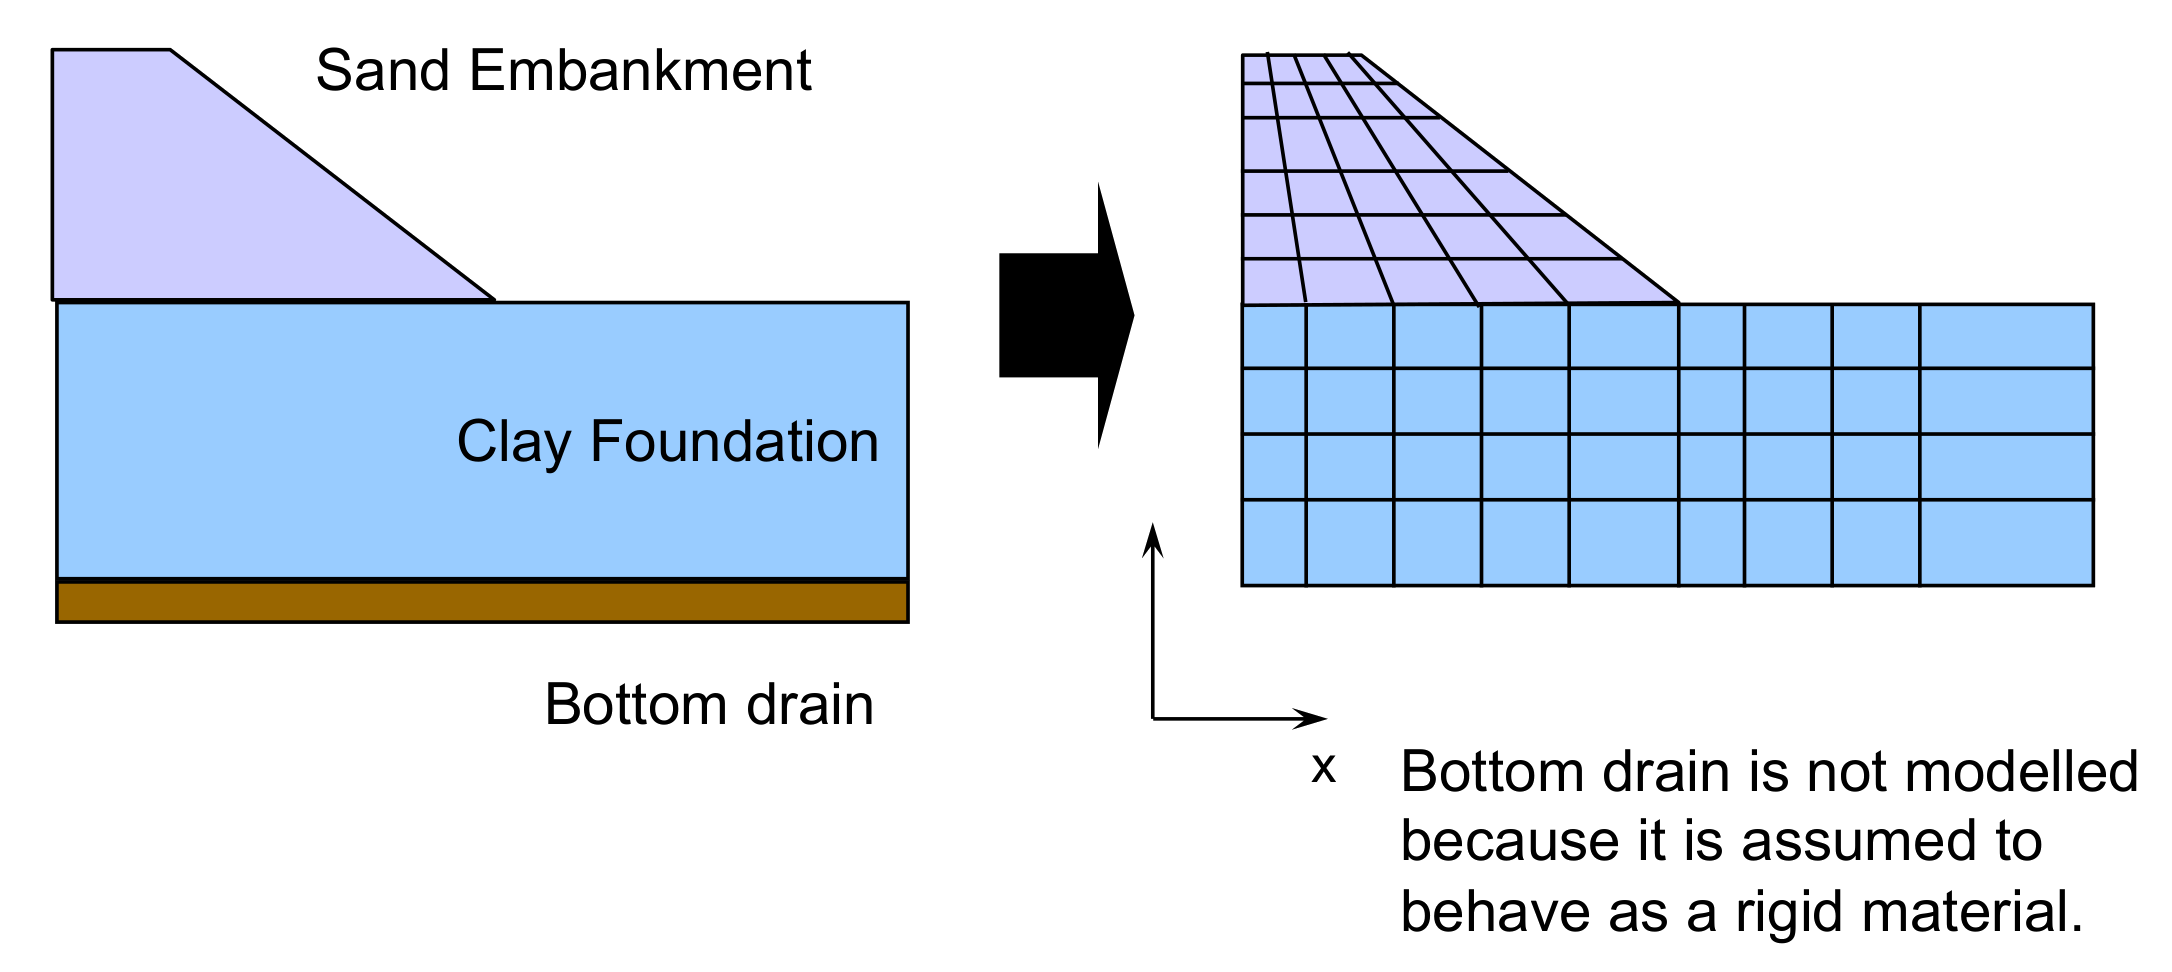
\includegraphics[width=0.9\textwidth]{figs/discretization.png}
\end{figure}
\end{frame}


%------------------------------------------------
\begin{frame}
\frametitle{FE discretization}
\mode<beamer>{
	\begin{figure}[ht]
		\centering
		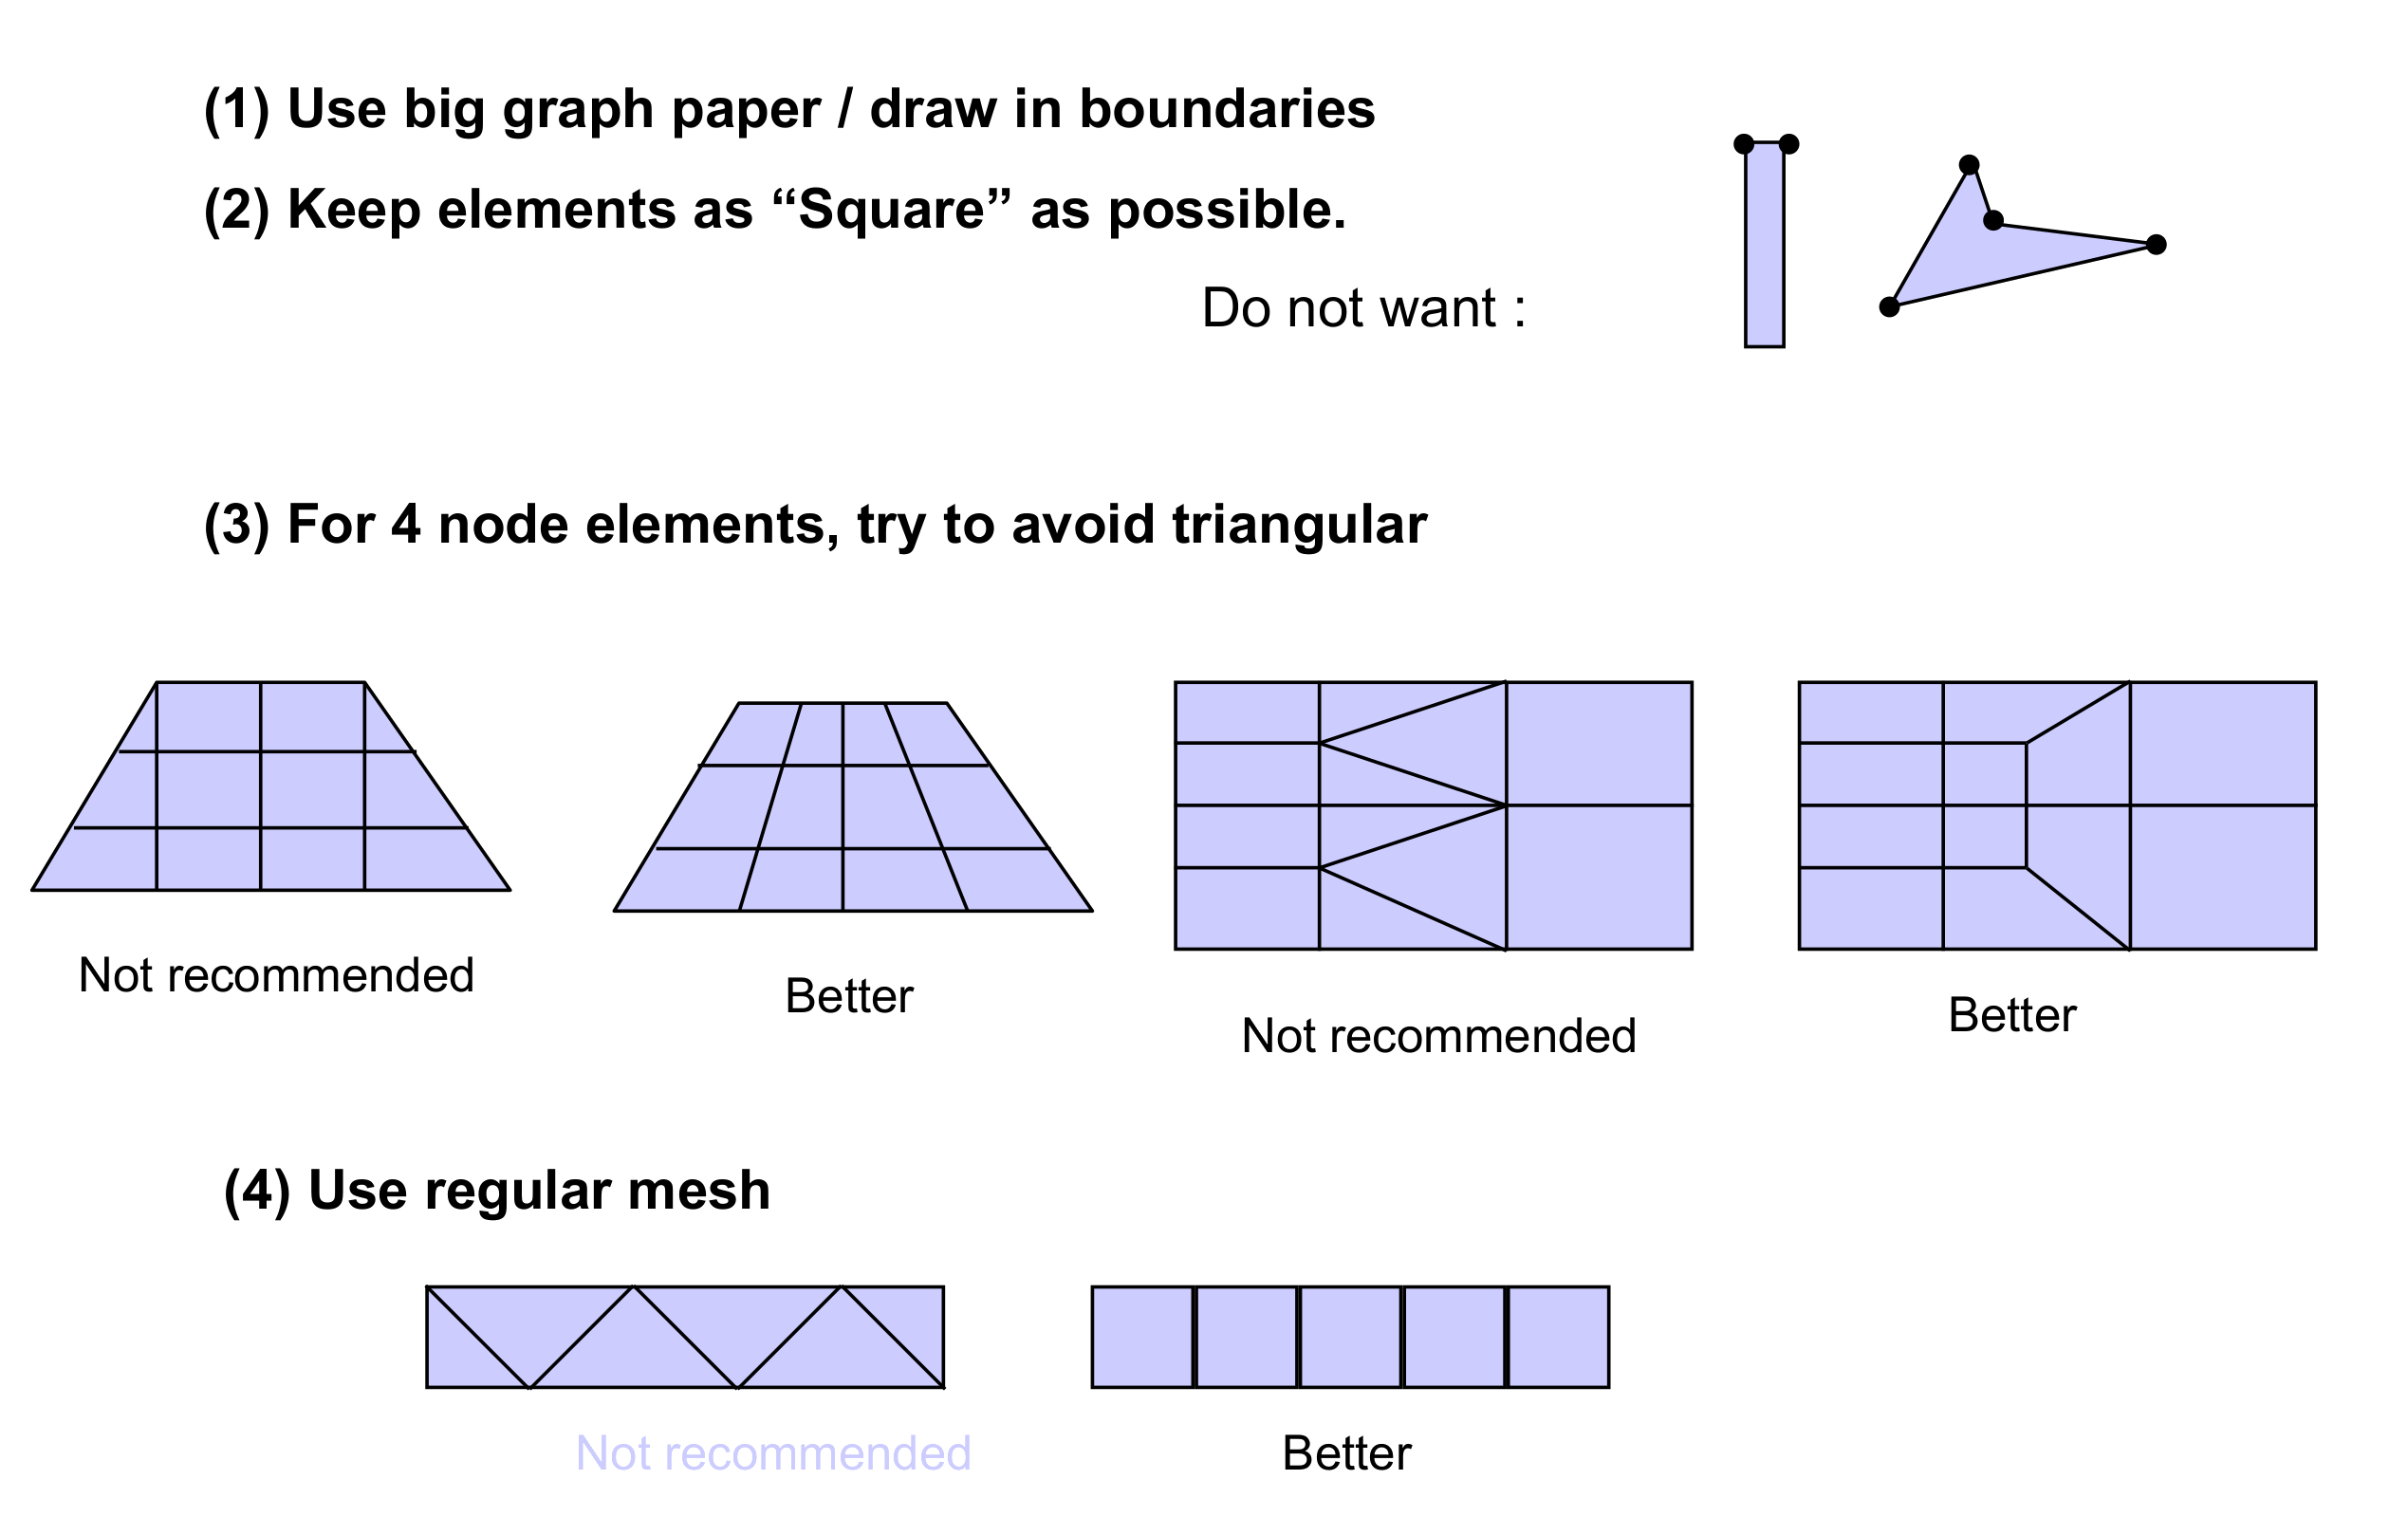
\includegraphics[width=\textwidth]{figs/fe-elements.png}
	\end{figure}
}
\mode<handout>{
	\begin{figure}[ht]
		\centering
		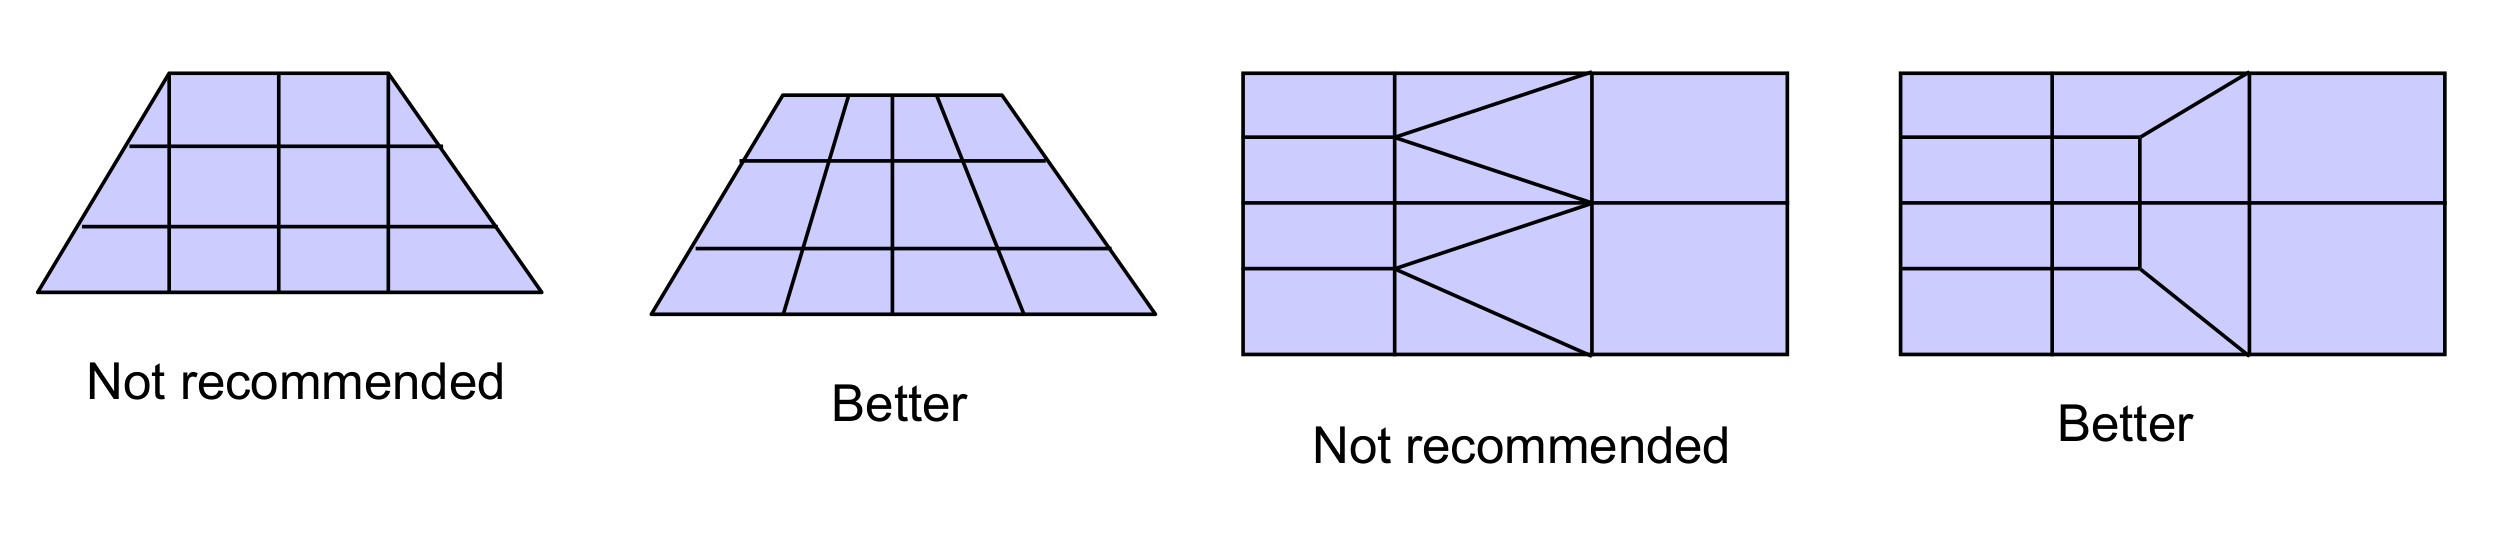
\includegraphics[width=\textwidth]{figs/good-fe-elements.png}
	\end{figure}
	\vspace{4cm}
}
\end{frame}

%------------------------------------------------
\begin{frame}
\frametitle{FE discretization: Refining}
\begin{figure}[ht]
	\centering
	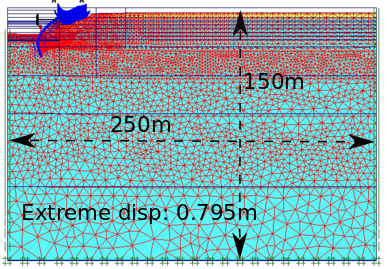
\includegraphics[width=0.8\textwidth]{figs/refined-mesh.png}
	\caption*{Avoid large jumps in element size: size jump should be < 3}
\end{figure}
\end{frame}

\subsection{Boundary conditions}
%------------------------------------------------
\begin{frame}
\frametitle{FE boundary conditions}
\begin{figure}[ht]
	\centering
	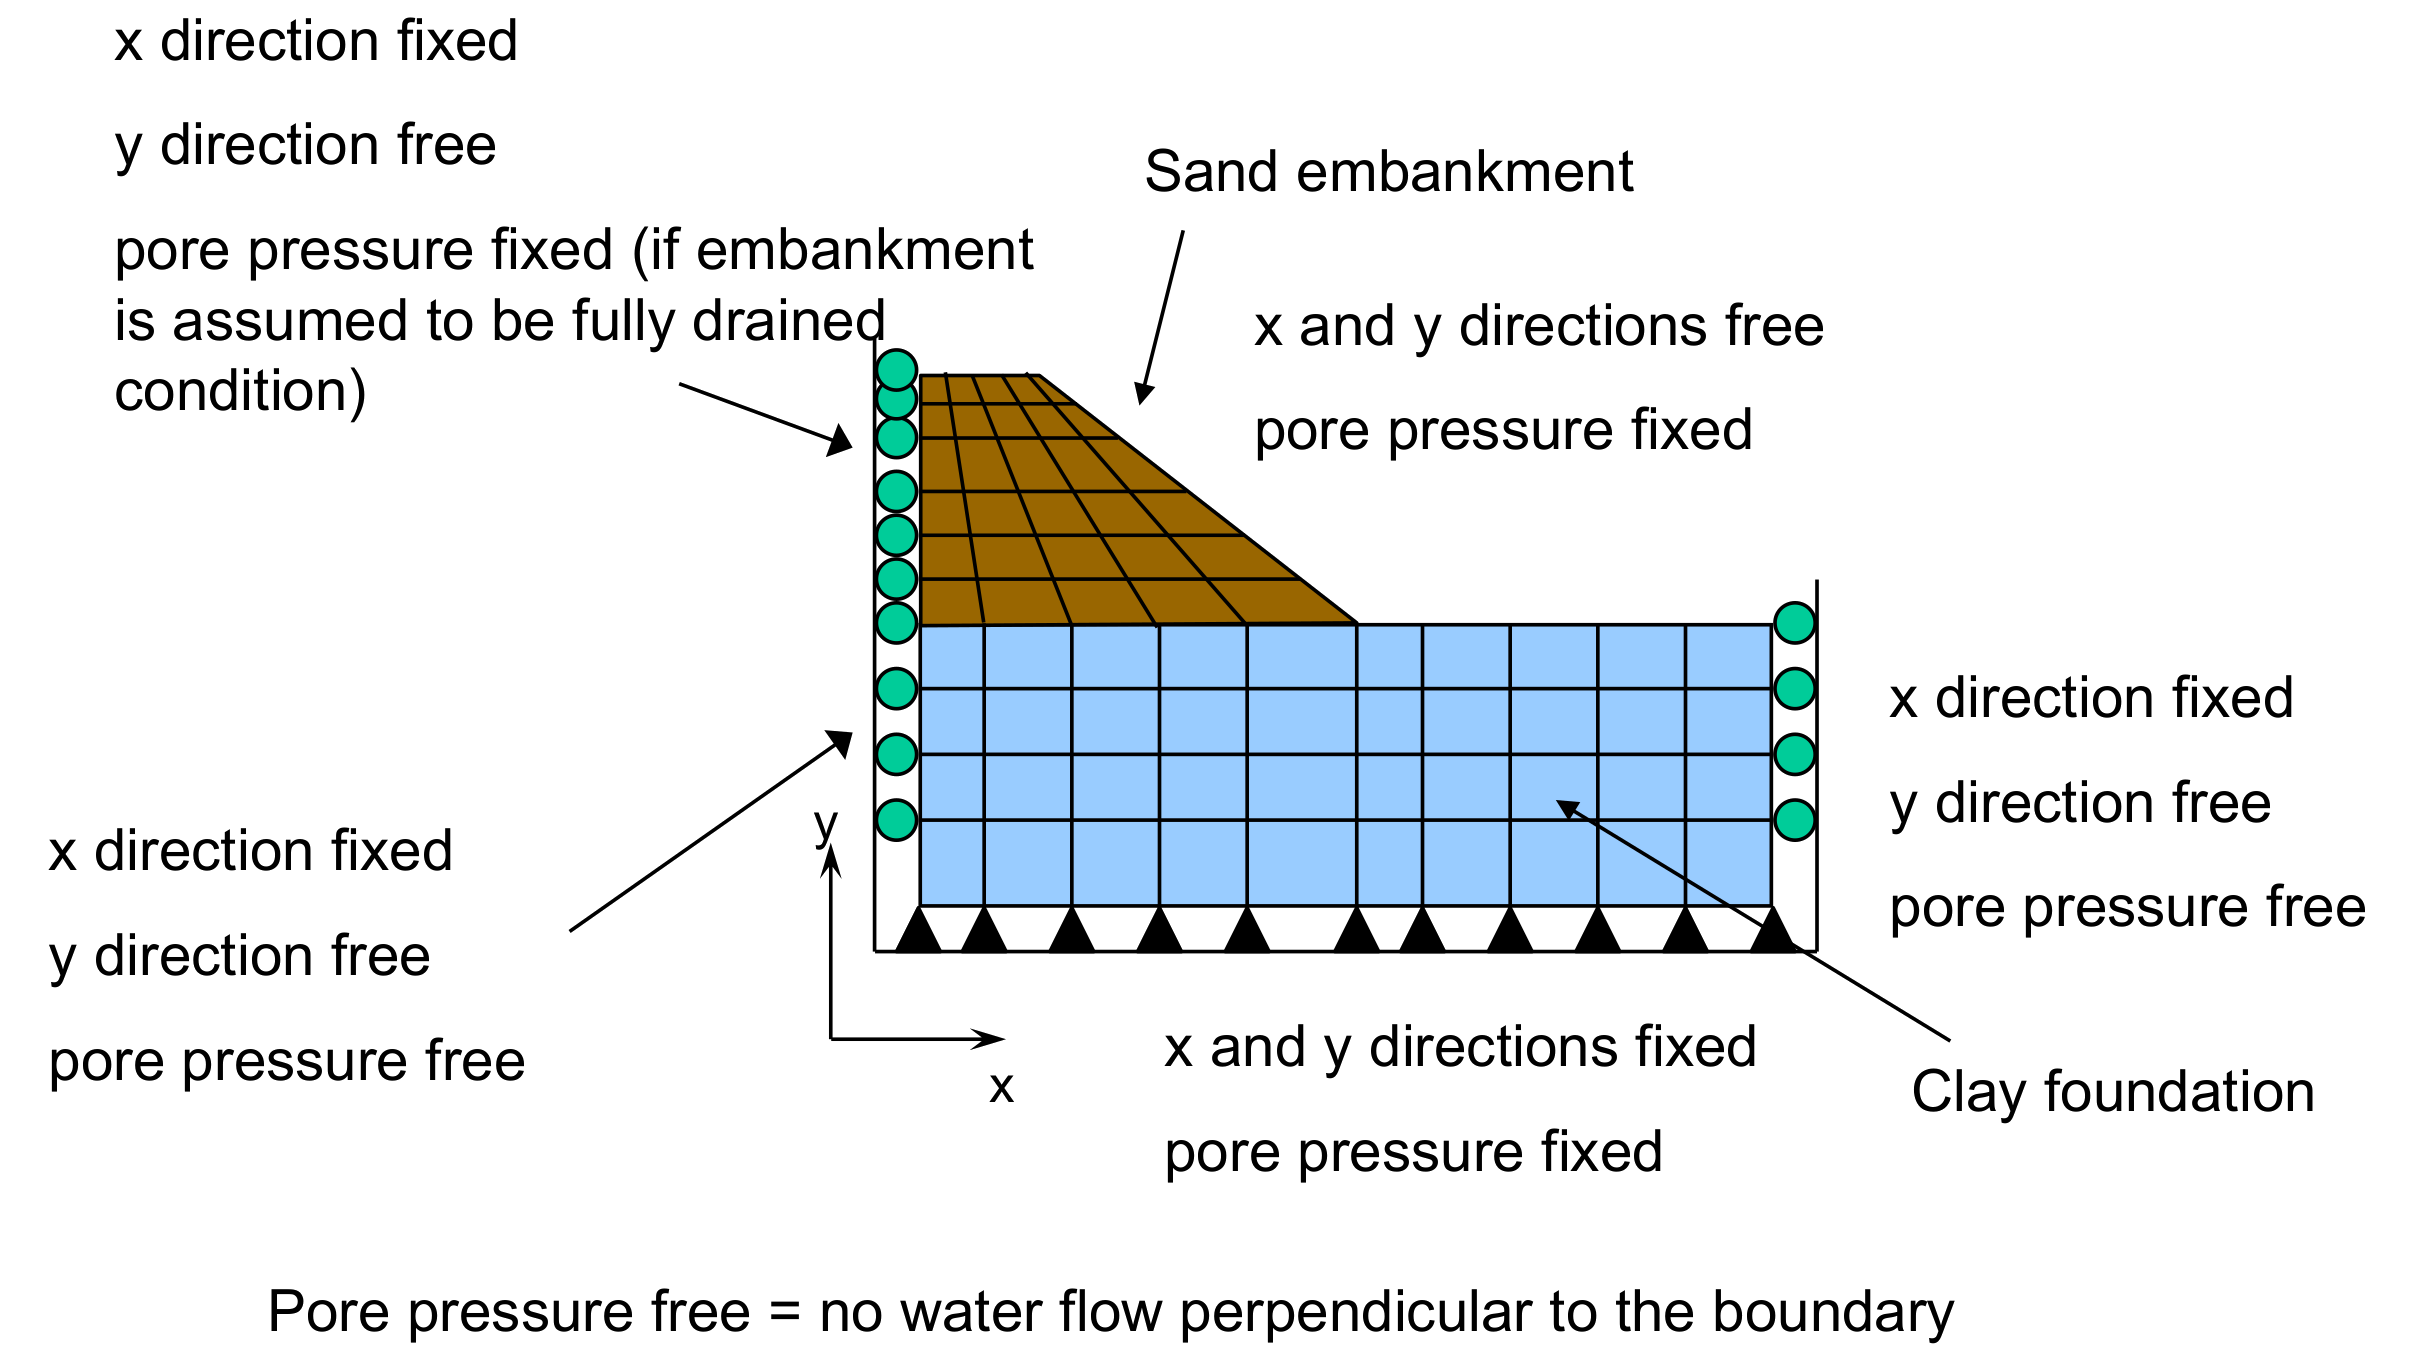
\includegraphics[width=\textwidth]{figs/boundary-conditions.png}
\end{figure}
\end{frame}

%------------------------------------------------
\begin{frame}
\frametitle{FE boundary conditions}
\begin{figure}[ht]
	\centering
	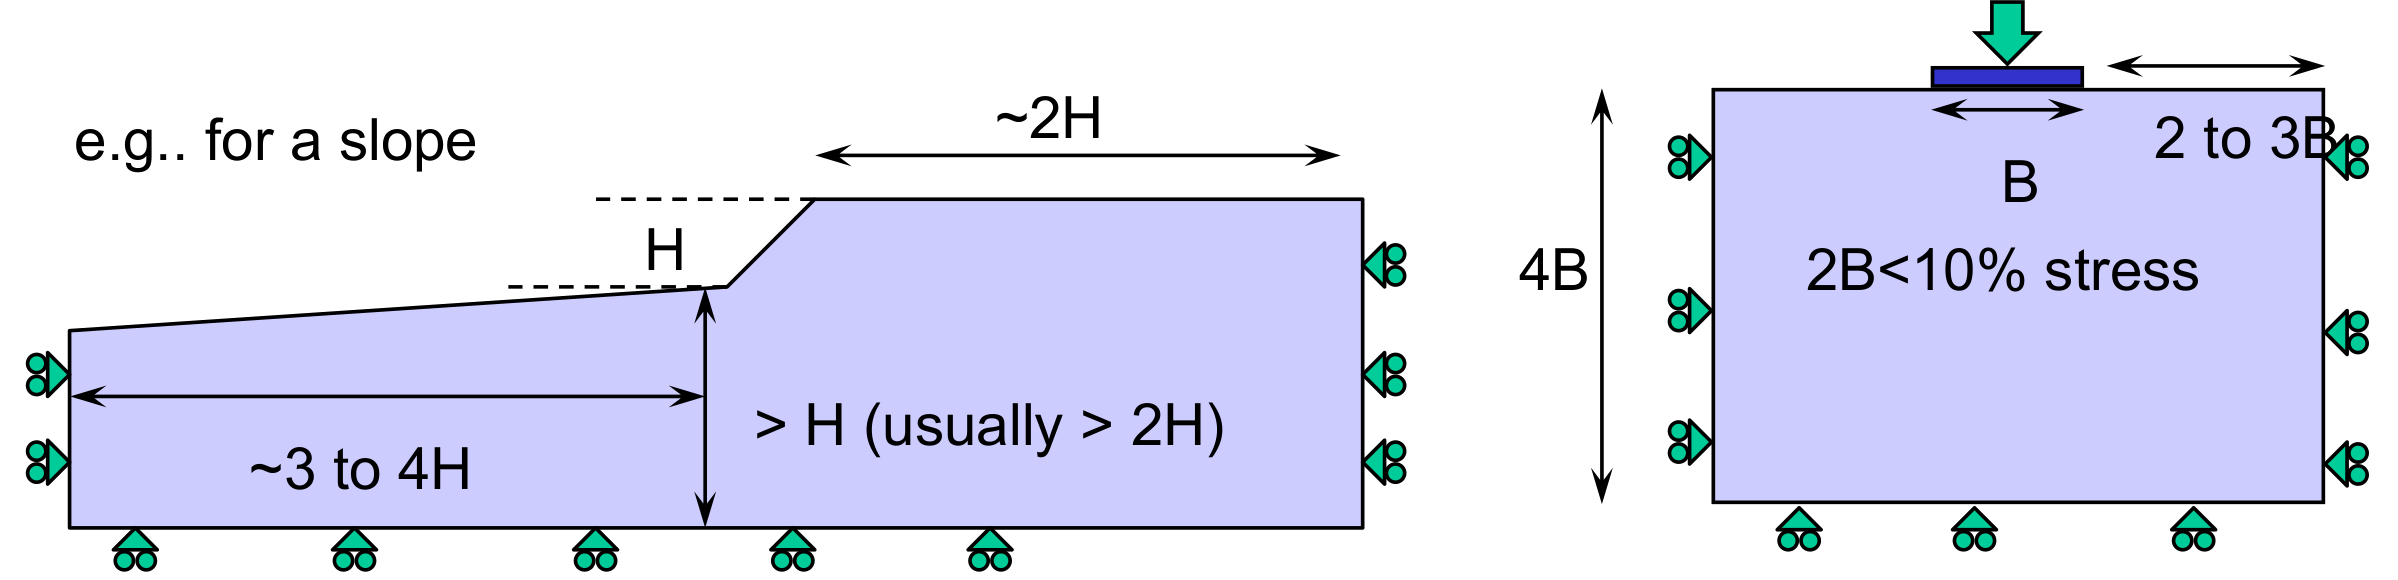
\includegraphics[width=\textwidth]{figs/fe-boundaries.png}
\end{figure}
\end{frame}

\subsection{Errors in FEA}
%------------------------------------------------
\begin{frame}
\frametitle{FE errors}
\mode<beamer>{
	\begin{figure}[ht]
		\centering
		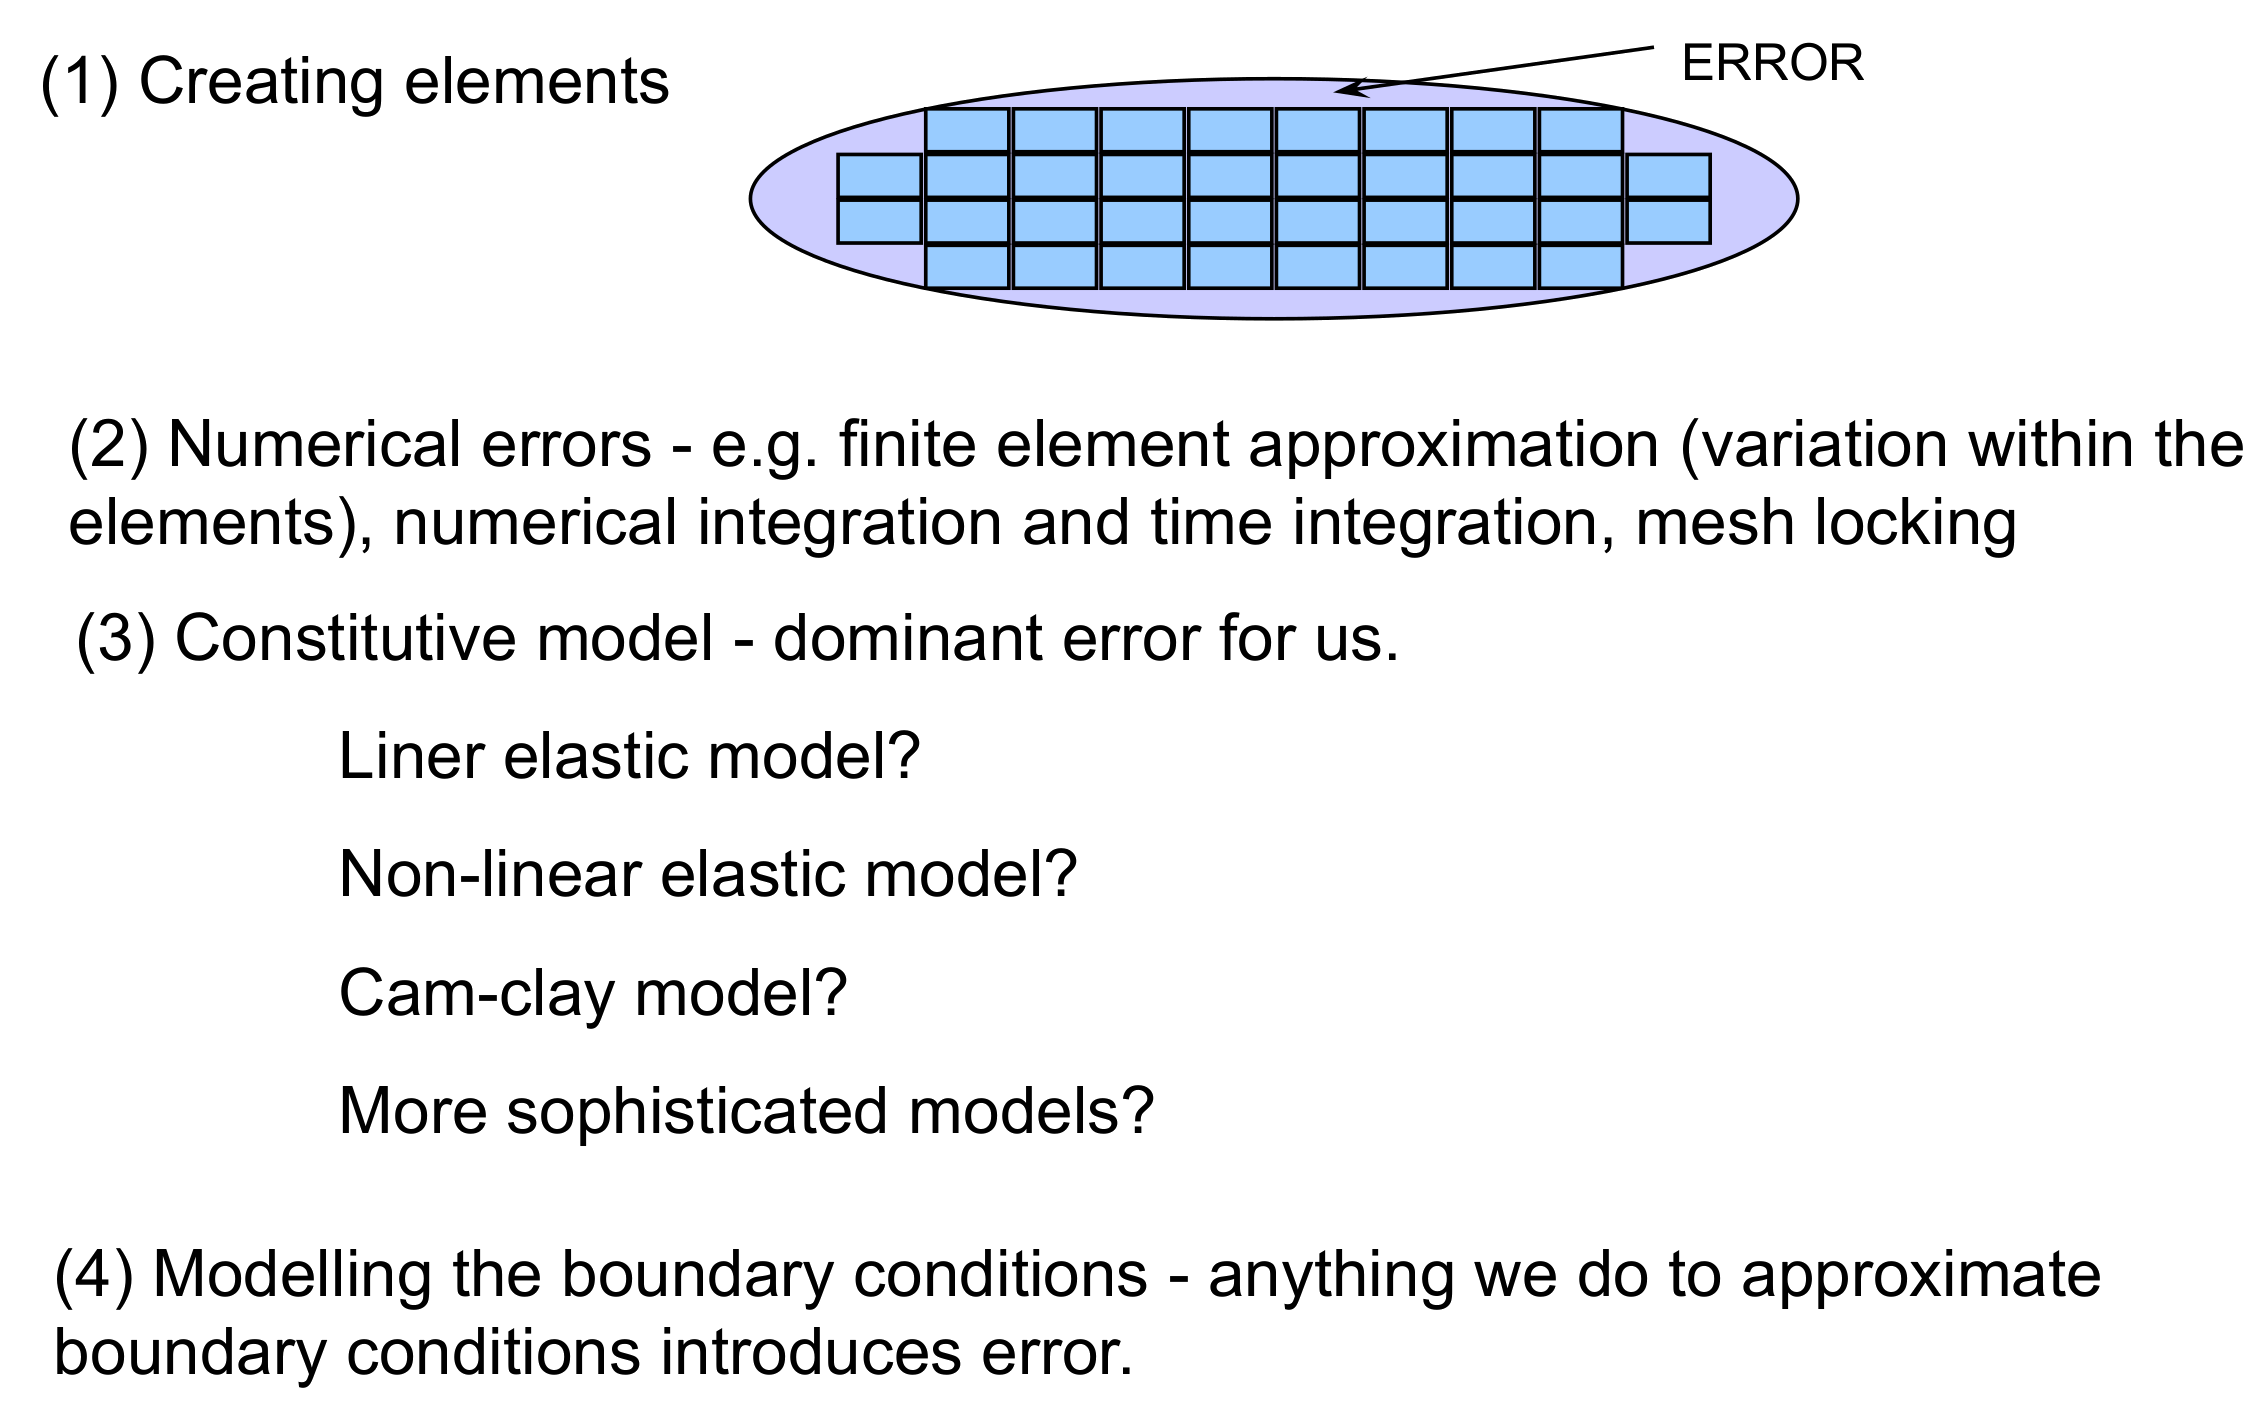
\includegraphics[width=0.9\textwidth]{figs/fe-errors.png}
	\end{figure}
}
\mode<handout>{
	\vspace{6cm}
}
\end{frame}

\section{Nicoll Highway Collapse, Singapore}
%------------------------------------------------
\begin{frame}
\frametitle{Nicoll Highway, Singapore}
\begin{figure}[ht]
	\centering
	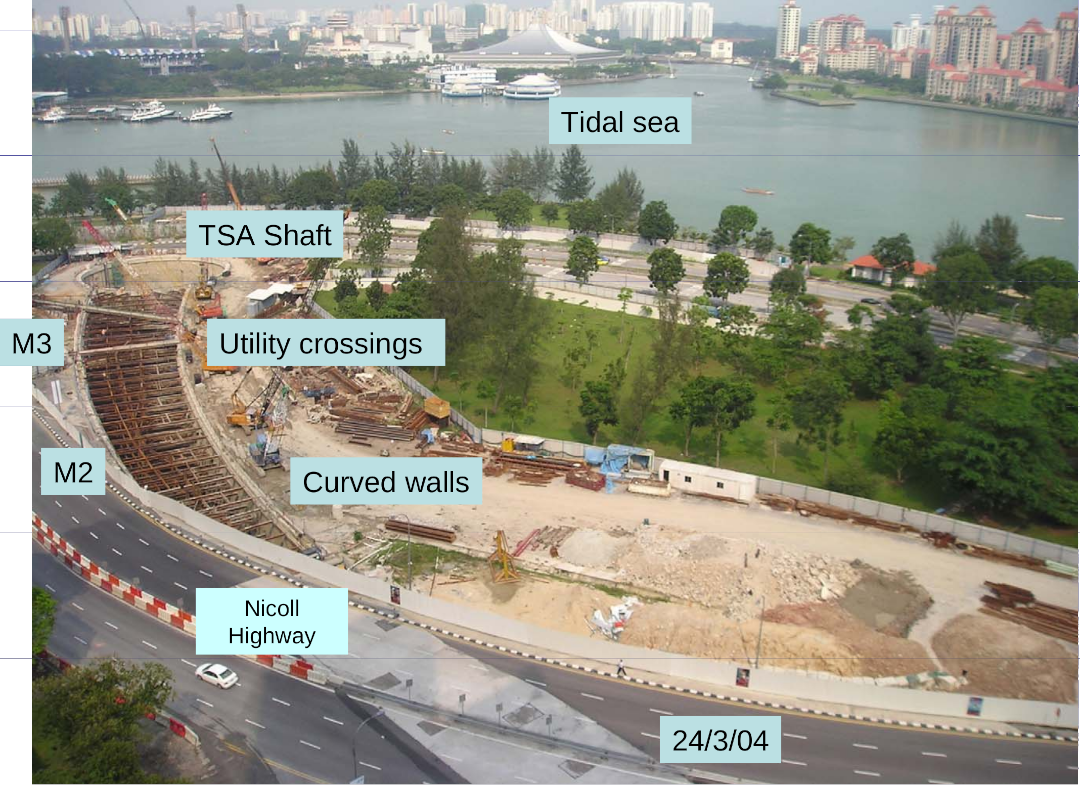
\includegraphics[width=0.9\textwidth]{figs/nicoll-highway.png}
	\caption{Thanks to GCG, DW Hight, TO Henderson, AR Pickes and S Marchand }
\end{figure}
\end{frame}

%------------------------------------------------
\begin{frame}
\frametitle{Nicoll Highway, Singapore}
\begin{figure}[ht]
	\centering
	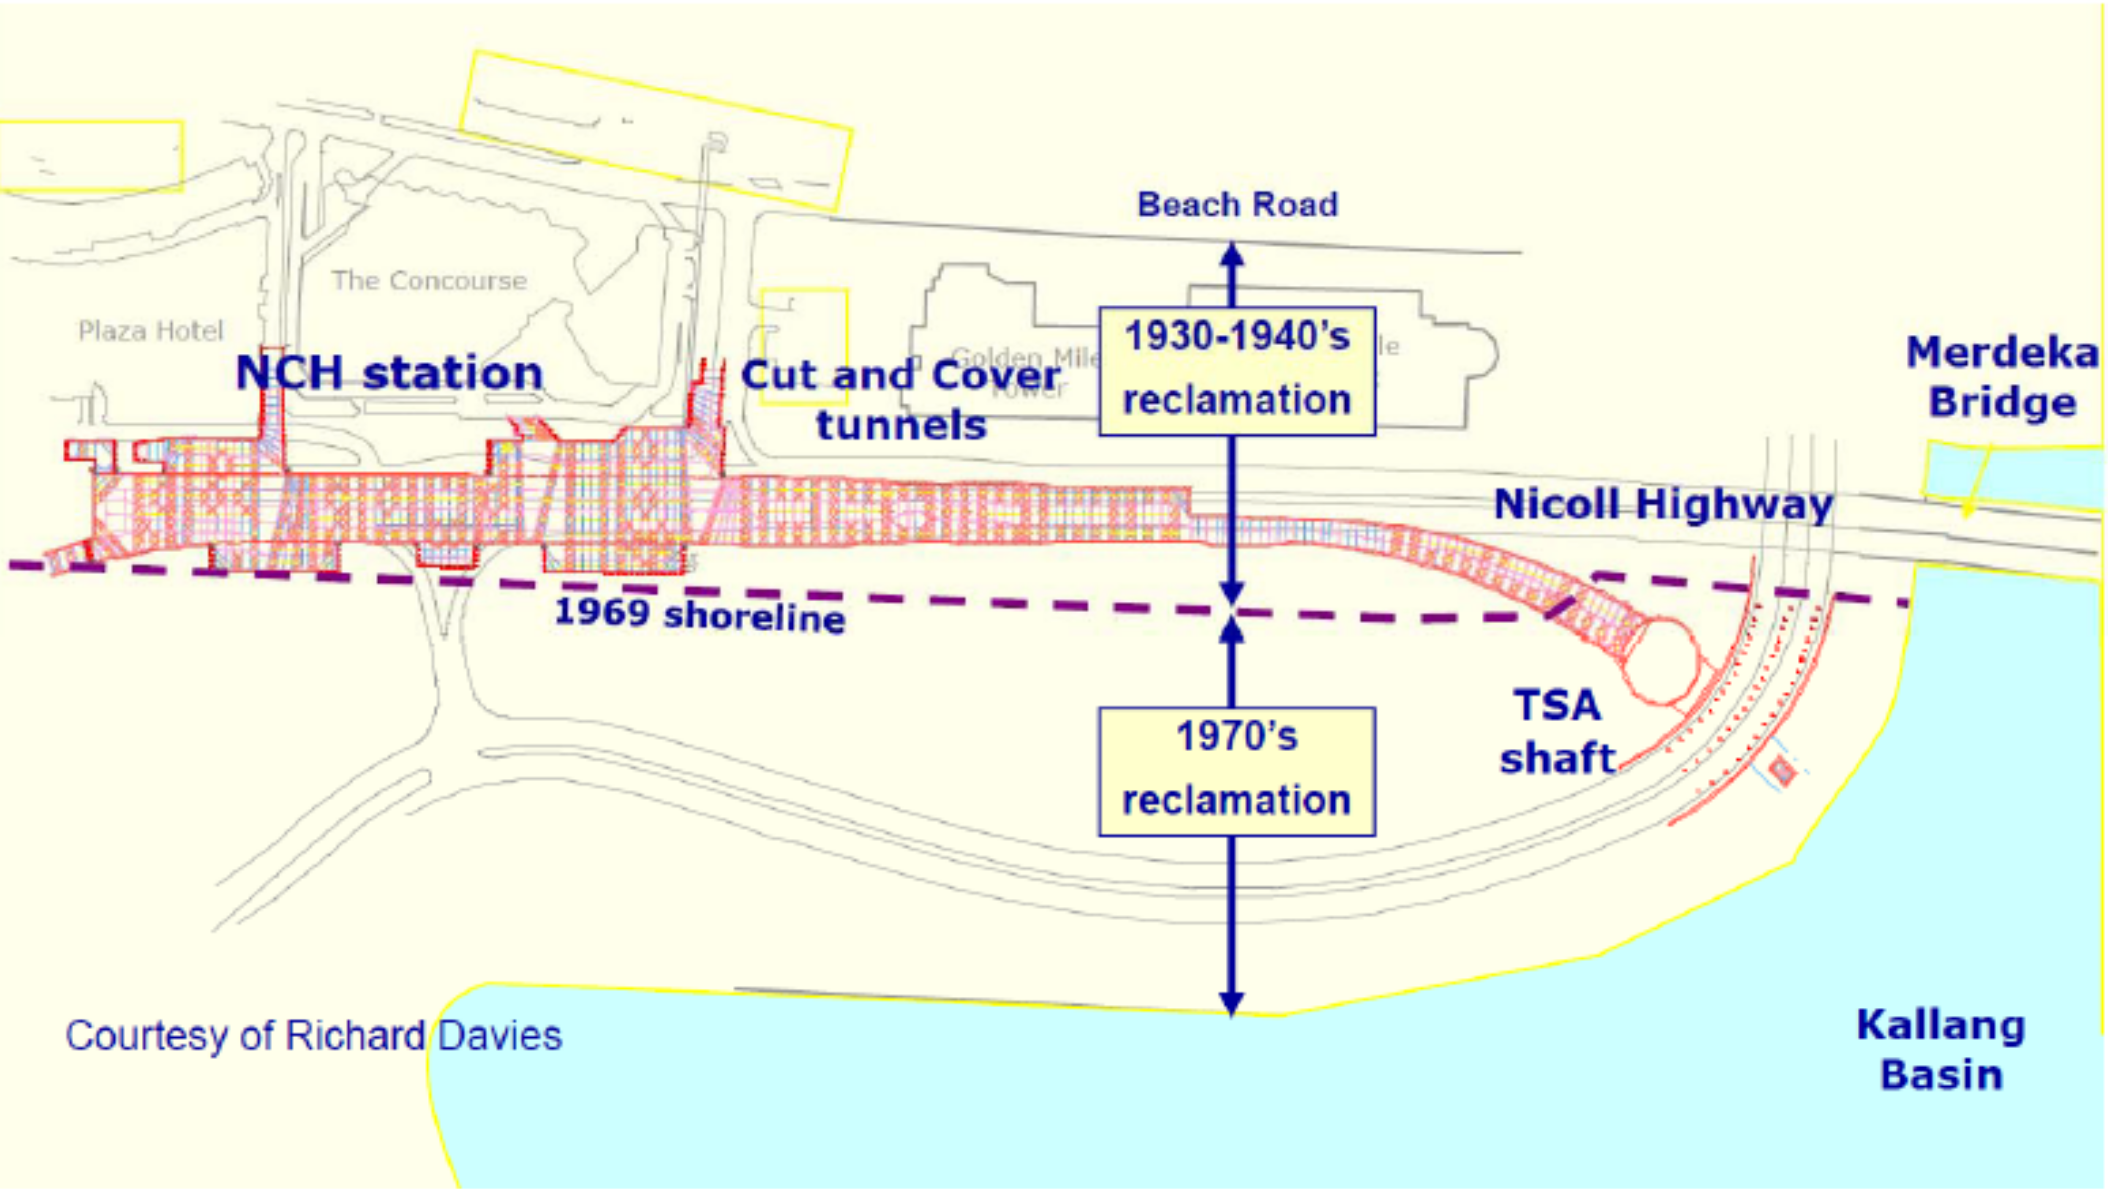
\includegraphics[width=0.9\textwidth]{figs/nicoll-plan-view.png}
\end{figure}
\end{frame}
	
\note{The tunnels were constructed on reclaimed lands. Reclamation was done in two stages. Northern part of the site was reclaimed over 50 years ago and the southern part was reclaimed about 20 years ago. Therefore the top soil of the collapse site comprised of fill material. Underneath the top layer there were layers of soft clays (marine clay and estuarine clay deposits) to a depth of 37-40 meters. Beneath these layers were layers of sands, silts, clays and an old alluvium formation. Ground water table was generally about 2 meters below the surface.}

%------------------------------------------------
\begin{frame}
\frametitle{Nicoll Highway, Singapore}
\begin{figure}[ht]
	\centering
	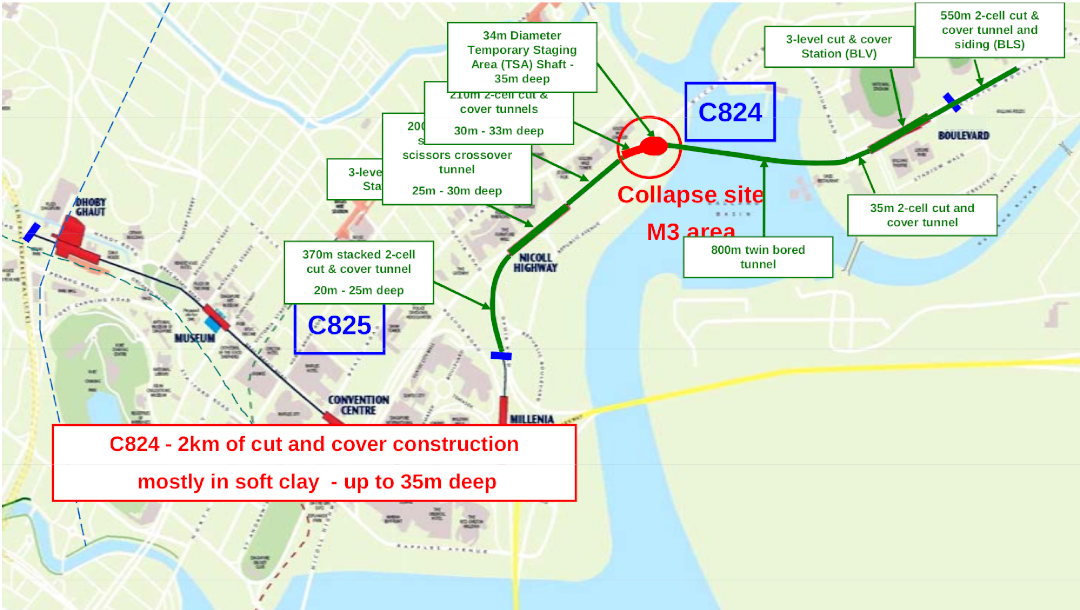
\includegraphics[width=0.9\textwidth]{figs/circle-line-stage1.png}
\end{figure}
\end{frame}

\note{The Mass Rapid Transit (MRT) rail network system is an integral part of Singapore’s public transport system. The MRT network involved construction of bored and cut and cover type tunnels. On the 20th of April 2004 at around 3:30 pm the temporary lateral support system of the cut and cover tunnel near the Nicoll Highway collapsed, resulting in the formation of a 100 ft. deep cave, which spread across six lanes of the Nicoll Highway. The collapse killed four people and injured three. The incident resulted in disruption of the gas, water and electric lines, which affected nearly 15000 people in the area. Two spans of a nearby bridge had to be demolished and reconstructed due to the damage in soil conditions the collapse had done in the nearby areas. One of the chief reasons for the failure of the temporary lateral support system was due to the overestimation of the undrained shear strength capacity of the soil.}

%------------------------------------------------
\begin{frame}
\frametitle{Cut and cover construction}
\end{frame}

\note{Construction of cut and cover tunnel involves building the tunnel structure inside an excavation. After the completion of the tunnel structure the excavation is covered with backfill material. Cut and cover type tunnels are typically constructed for depths of up to 30-40 feet. There are two approaches to the construction of a cut and cover tunnel (FHA Handbook 2009, pp 5-1-5-12).
	a) The Bottom-Up Method.
	b) The Top-Down Method.
}

\note{\textbf{Bottom-Up method}
	Bottom-up method involves excavation of a trench from the surface. The sides of the excavation can be sloped or vertical. The tunnel is then constructed in the trench and after the completion of the tunnel the trench is backfilled. Generally in urban areas due to limited availability of space the tunnel is often constructed with a vertical excavation supported by excavation support system. Excavation support system can be temporary or permanent. Some of the temporary excavation systems are sheet pile walls with multi levels of bracing, soldier piles with lagging walls, tieback support systems. Permanent excavation support systems form the part of the final tunnel structure. Some of the permanent excavation support systems are slurry walls, tangent pile wall support and soldier pile tremie concrete.
}

\note{
	\textbf{Top-Down method}
	Top-down method involves the construction of the tunnel walls, which are made using slurry walls, secant pile walls. After the construction of the tunnel walls the roof slab is constructed on the ground and connected with the tunnel walls. The roof slab is then covered and the surface of the ground can be used. Rest of the tunnel is excavated below the protection of the roof slab and the tunnel walls. After the excavation the rest of the tunnel can be finished and the floor slab can be constructed. This method is challenging to construct but the ground surface above the tunnel can be restored earlier.
	Bottom-Up method was used to construct the part of the cut and cover tunnel near Nicoll highway. Diaphragm walls supported the sides of the excavation and multi-levels of bracing were constructed as the excavation progressed.
	
}

%------------------------------------------------
\begin{frame}
\frametitle{Soil profile}
\begin{figure}[ht]
	\centering
	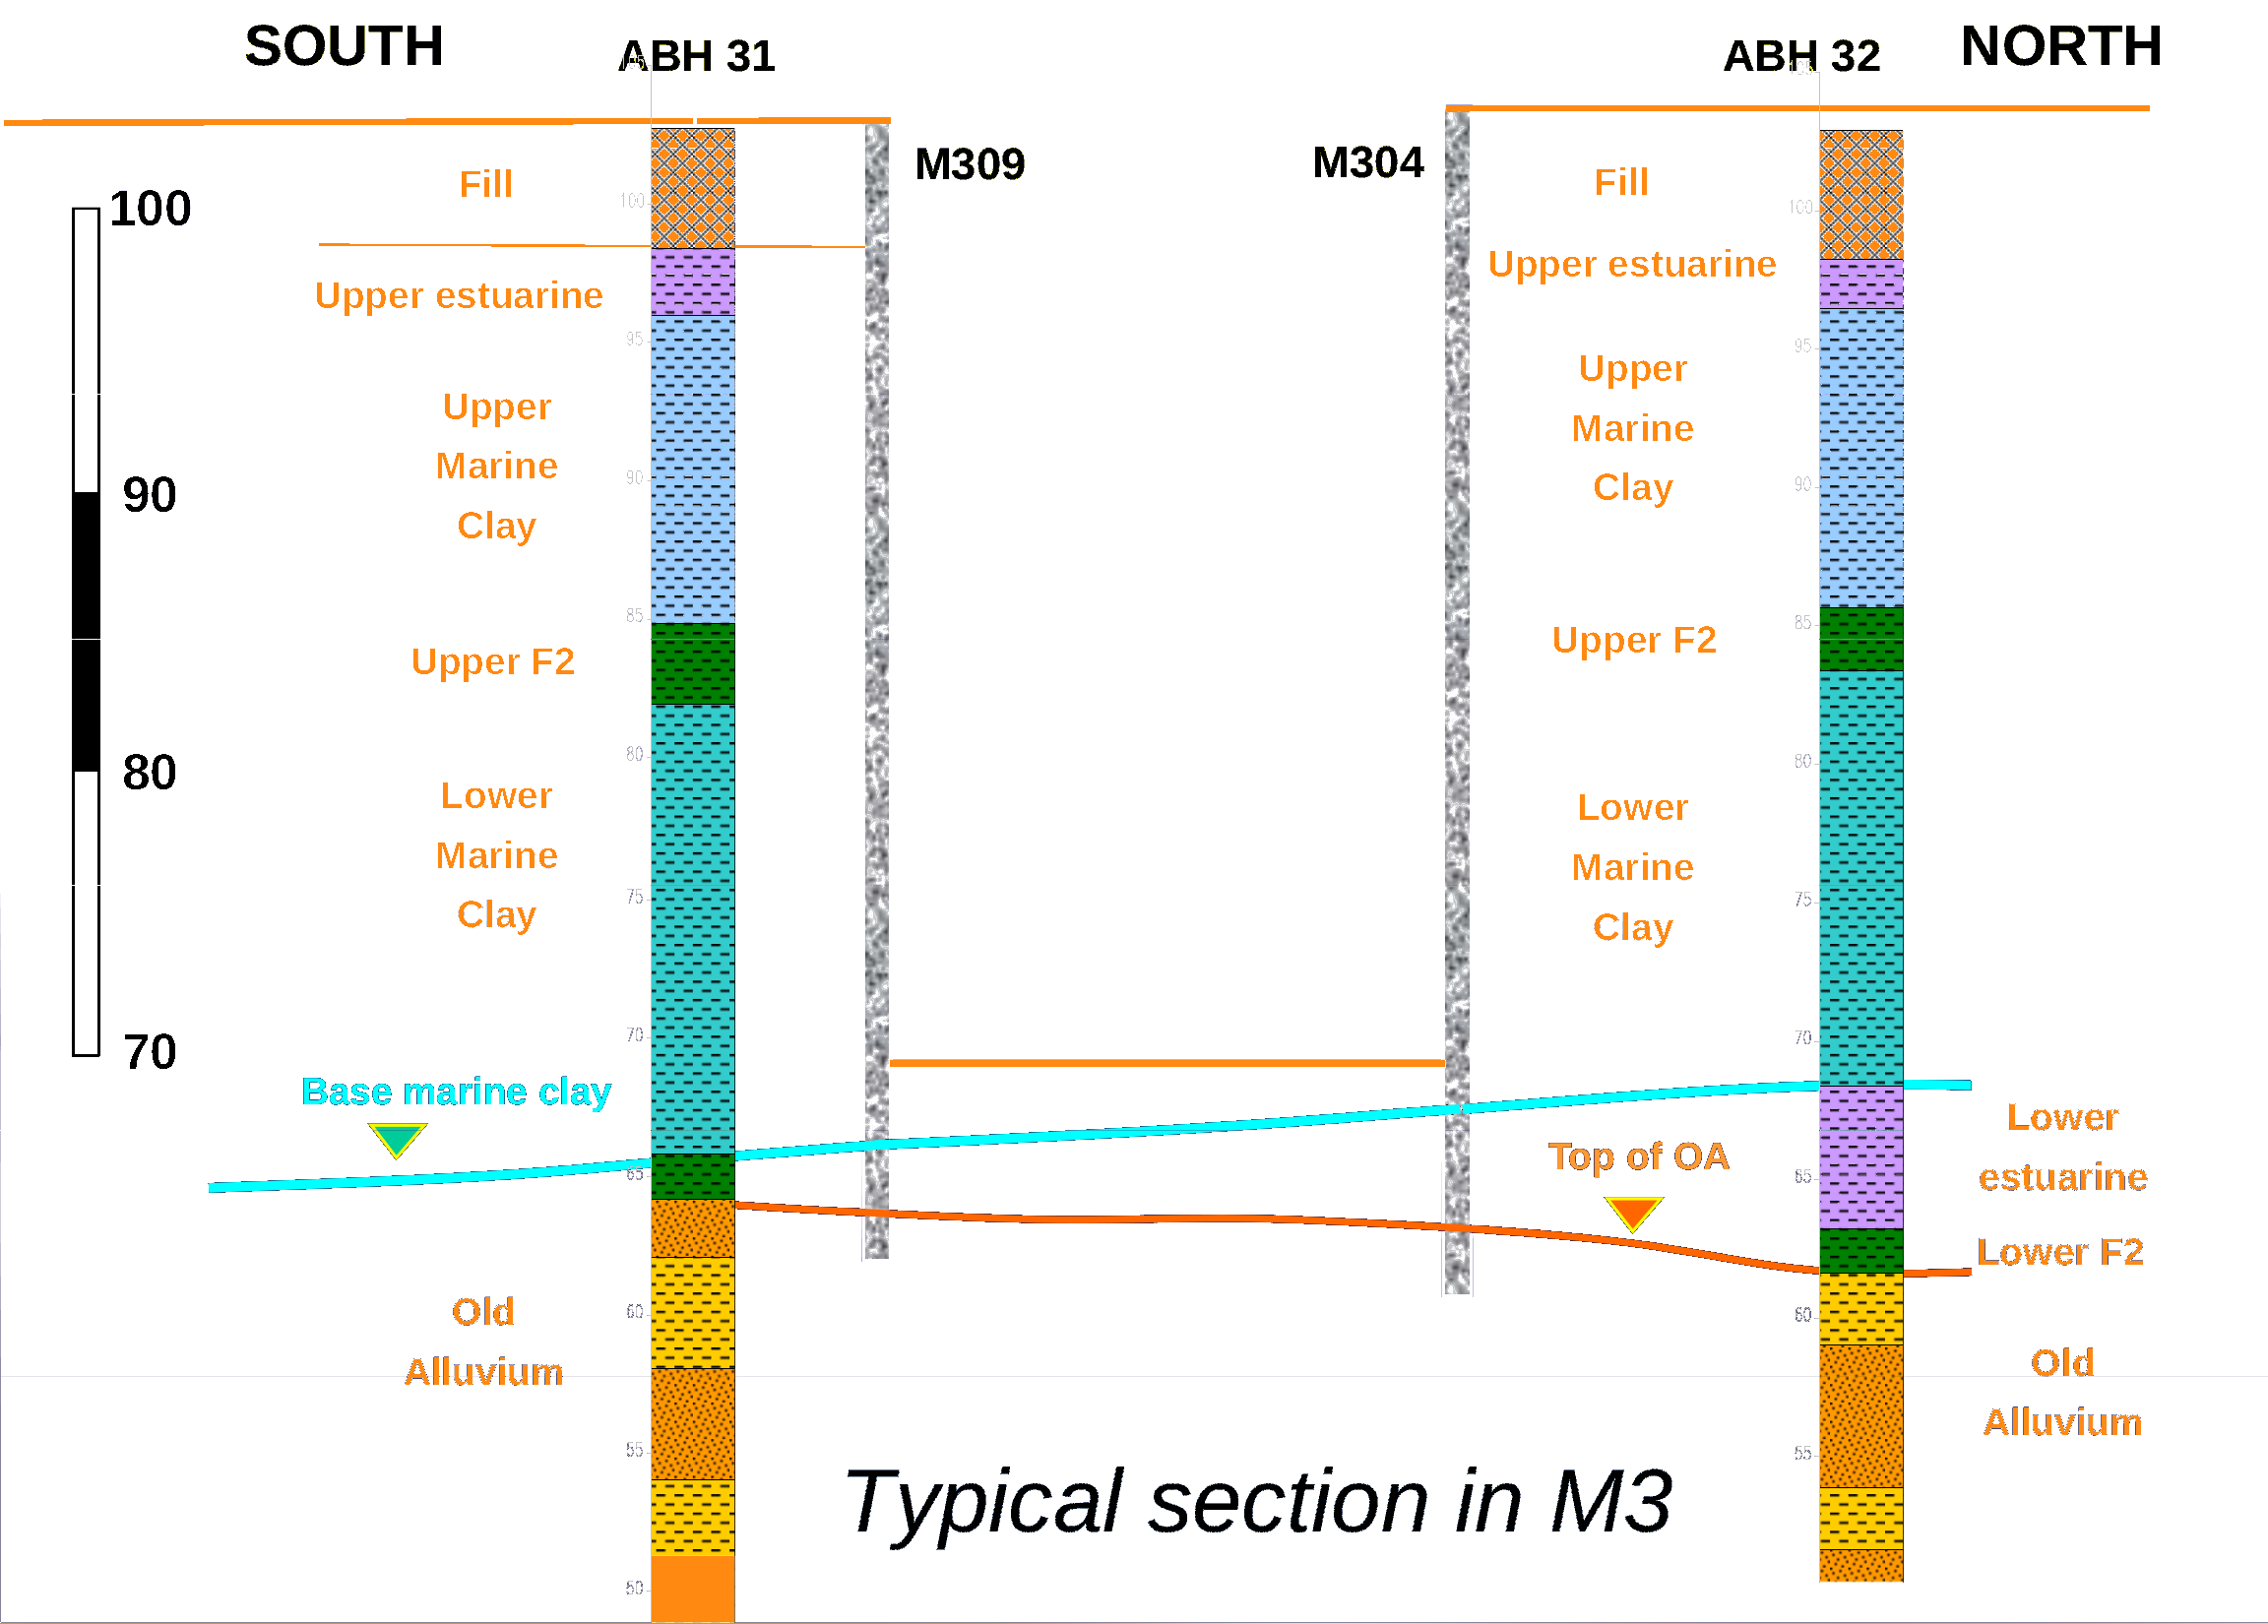
\includegraphics[width=0.85\textwidth]{figs/profile.png}
\end{figure}
\end{frame}

\note{
	The investigation included 14 boreholes and cone penetration tests along with collection of soil samples and testing them in laboratories. After the contract was awarded an extensive testing was conducted which included 72 boreholes and cone penetration tests to determine the alignment of the tunnel and get data for the purpose of design (COI 2005, pp 16-35).
}

%------------------------------------------------
\begin{frame}
\frametitle{Construction sequence}
\begin{figure}[ht]
	\centering
	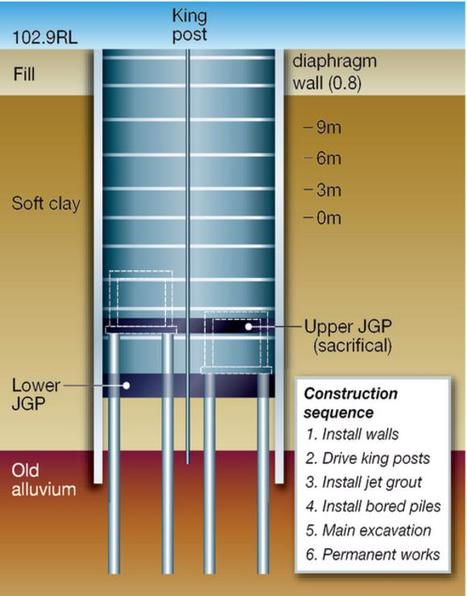
\includegraphics[width=0.5\textwidth]{figs/construction-sequence.jpg}
\end{figure}
\end{frame}

\note{For design purposes diaphragm walls were divided into 40 different wall sections. Wall sections were designed based on the worst soil parameters obtained from the nearest borehole. The temporary retaining wall system consisting of diaphragm walls and struts was modeled, analyzed and designed using Plaxis, which is a widely used geotechnical modeling software based on finite element method. Soil layers were modeled using Mohr-Coulomb soil model with effective stress strength parameters. \textbf{A load factor of 1.2} was considered for obtaining the design forces on the diaphragm. \textbf{Diaphragm wall designs were optimized based on the wall movement criteria, with maximum allowable movement being 200 mm at any depth of the wall and 40 mm at the diaphragm wall toe.}}

\note{
There were two layers of interlocking jet grout piles. The upper layer of the jet grout pile was 1.5 m thick and was temporary and the lower layer of the jet grout pile was 2.5 m thick and formed the base of the tunnel. Jet grout pile layers were built to minimize the deflection of the walls while the tunnel was being excavated. Bored piles were constructed to support the rail boxes. Excavation was supported by a system of steel king post and 10 levels of struts placed at 4m center to center. As the excavation progressed the struts were constructed and before the construction of the 10th level of strut the temporary layer of the jet gout pile was removed.\\

The entire process of tunnel construction was monitored by thousands of geotechnical instruments including settlement markers, inclinometers to monitor the soil and wall deflections, vibrating wire piezometers, strain gauges and load cells. The instruments installed in the failed part of the tunnel section provided data, which helped to understand the reasons for the collapse. 
}


%------------------------------------------------
\begin{frame}
\frametitle{Construction sequence}
\begin{figure}[ht]
	\centering
	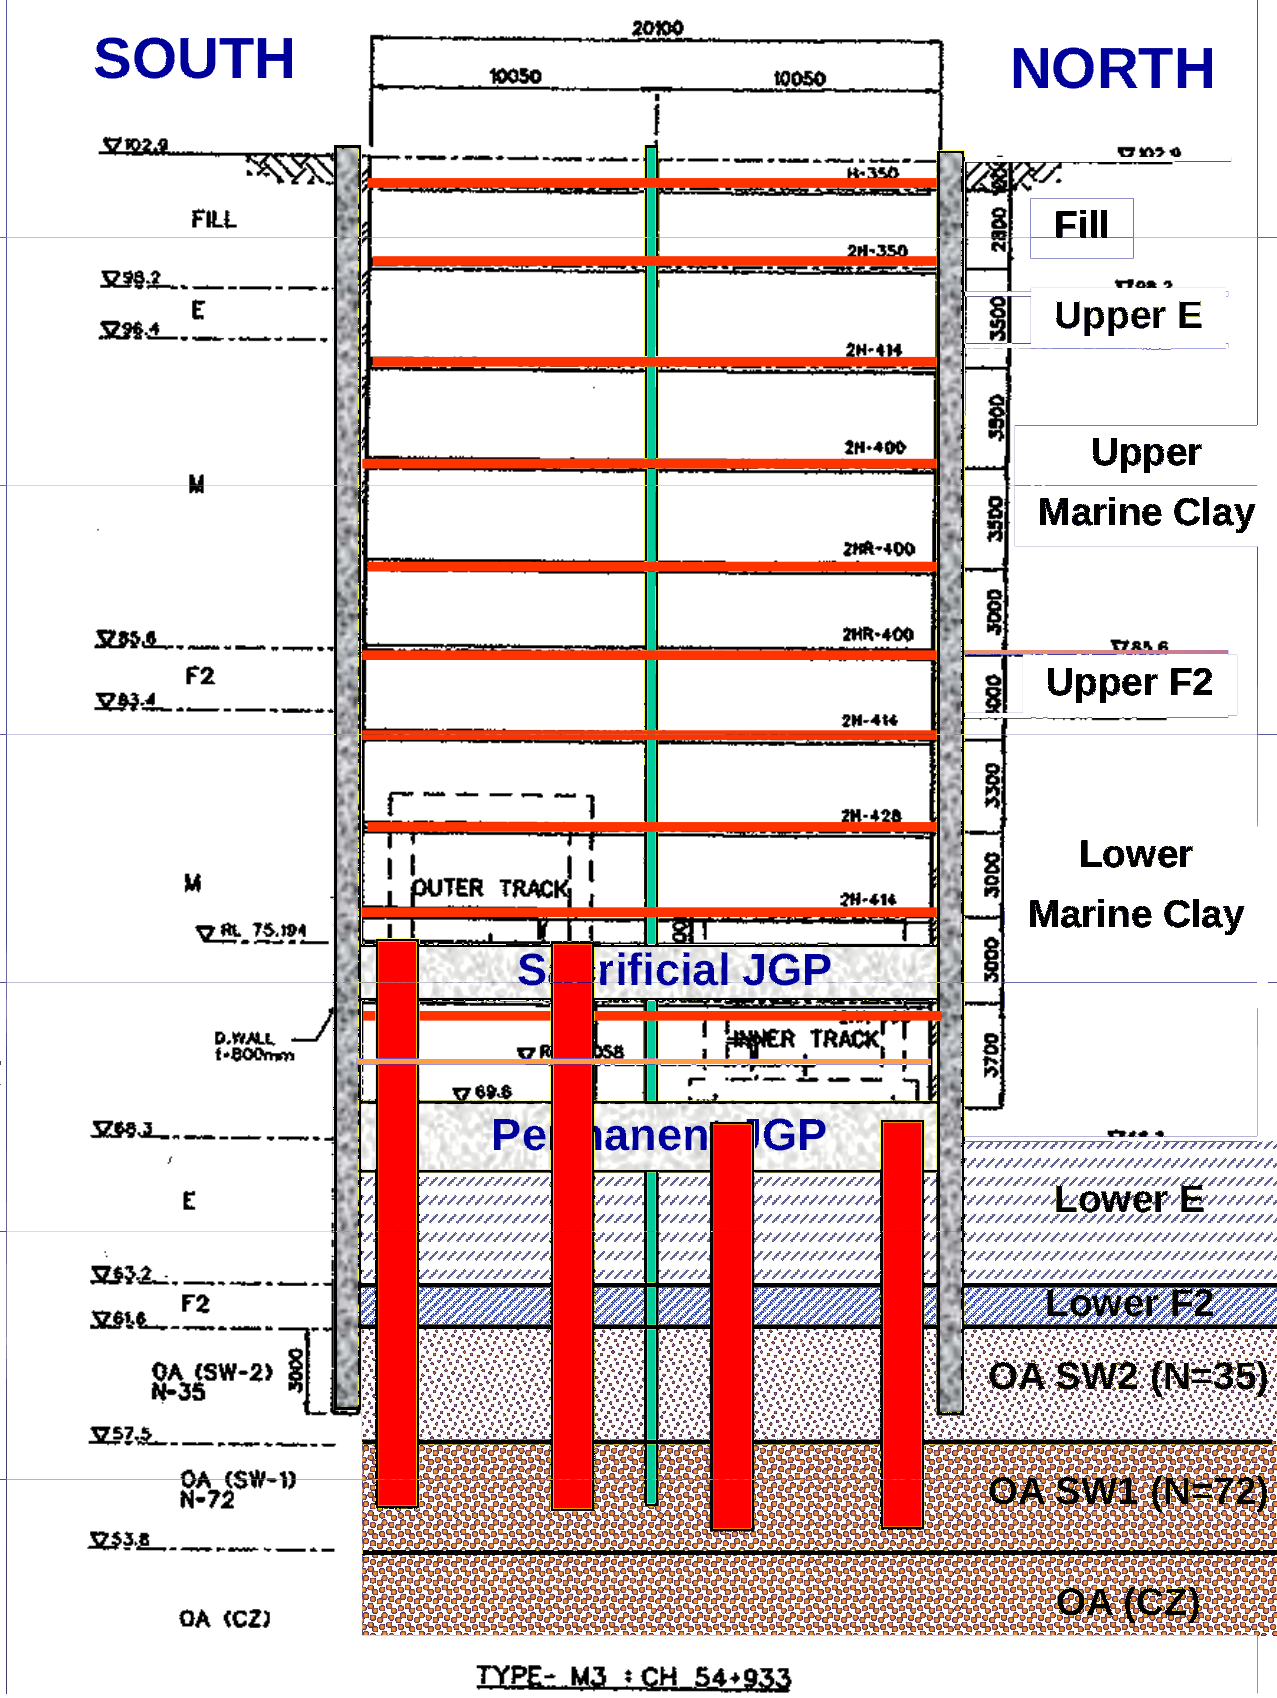
\includegraphics[width=0.5\textwidth]{figs/excavation-stages.png}
\end{figure}
\end{frame}

%------------------------------------------------
\begin{frame}
\frametitle{Nicoll Highway: Excavation}
\begin{figure}[ht]
	\centering
	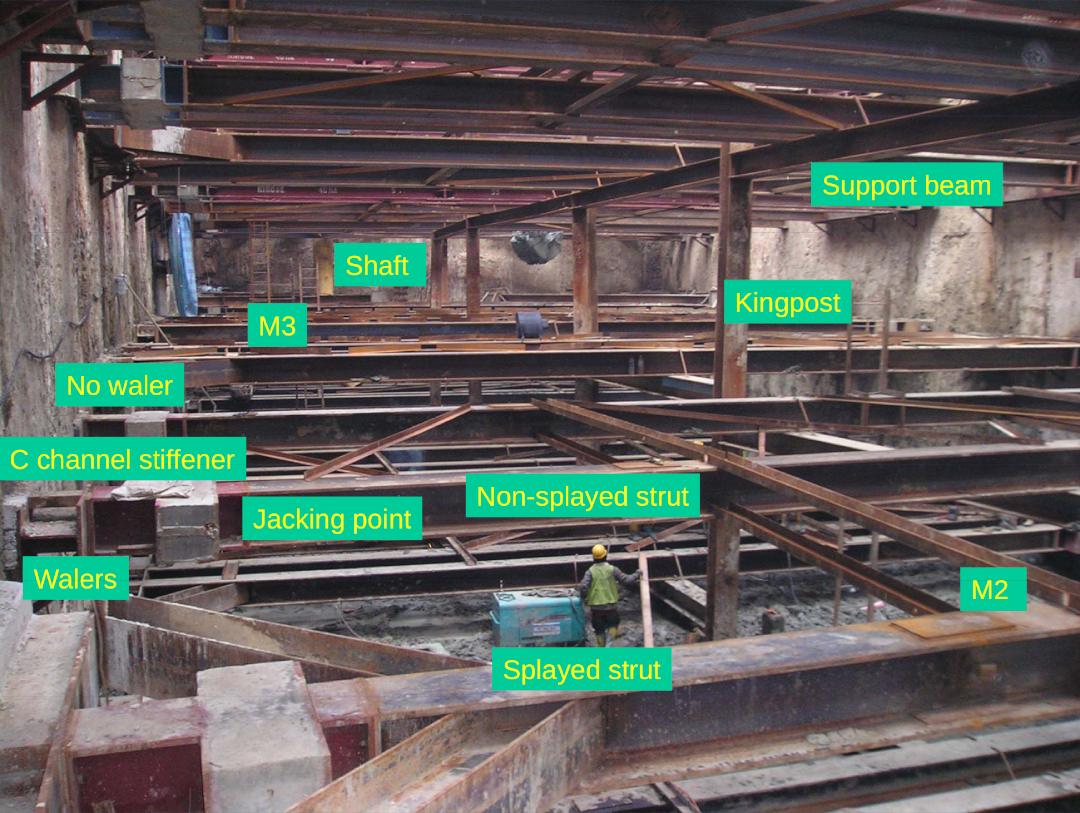
\includegraphics[width=0.9\textwidth]{figs/nicoll-highway-structures.png}
\end{figure}
\end{frame}

%------------------------------------------------
\begin{frame}
\frametitle{South side 13 March 2004}
\begin{figure}[ht]
	\centering
	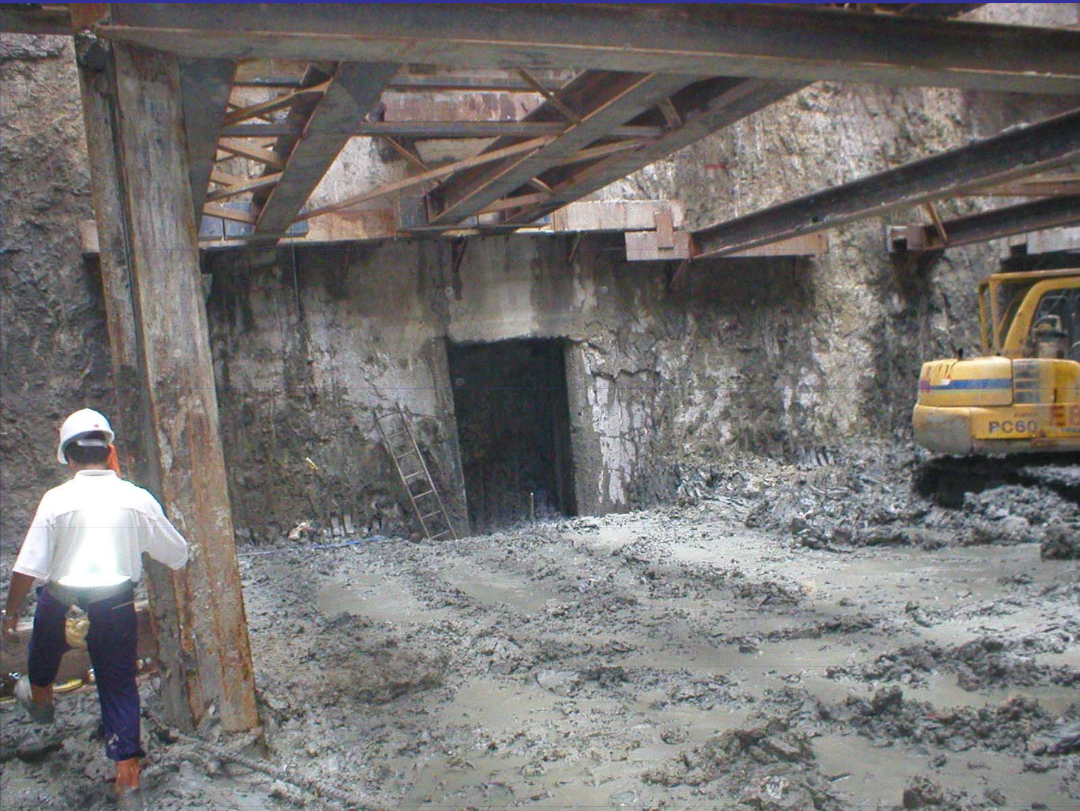
\includegraphics[width=0.8\textwidth]{figs/south-side-14march04.png}
\end{figure}
\end{frame}

%------------------------------------------------
\begin{frame}
\frametitle{Excavating 10th level of struts}
\begin{figure}[ht]
	\centering
	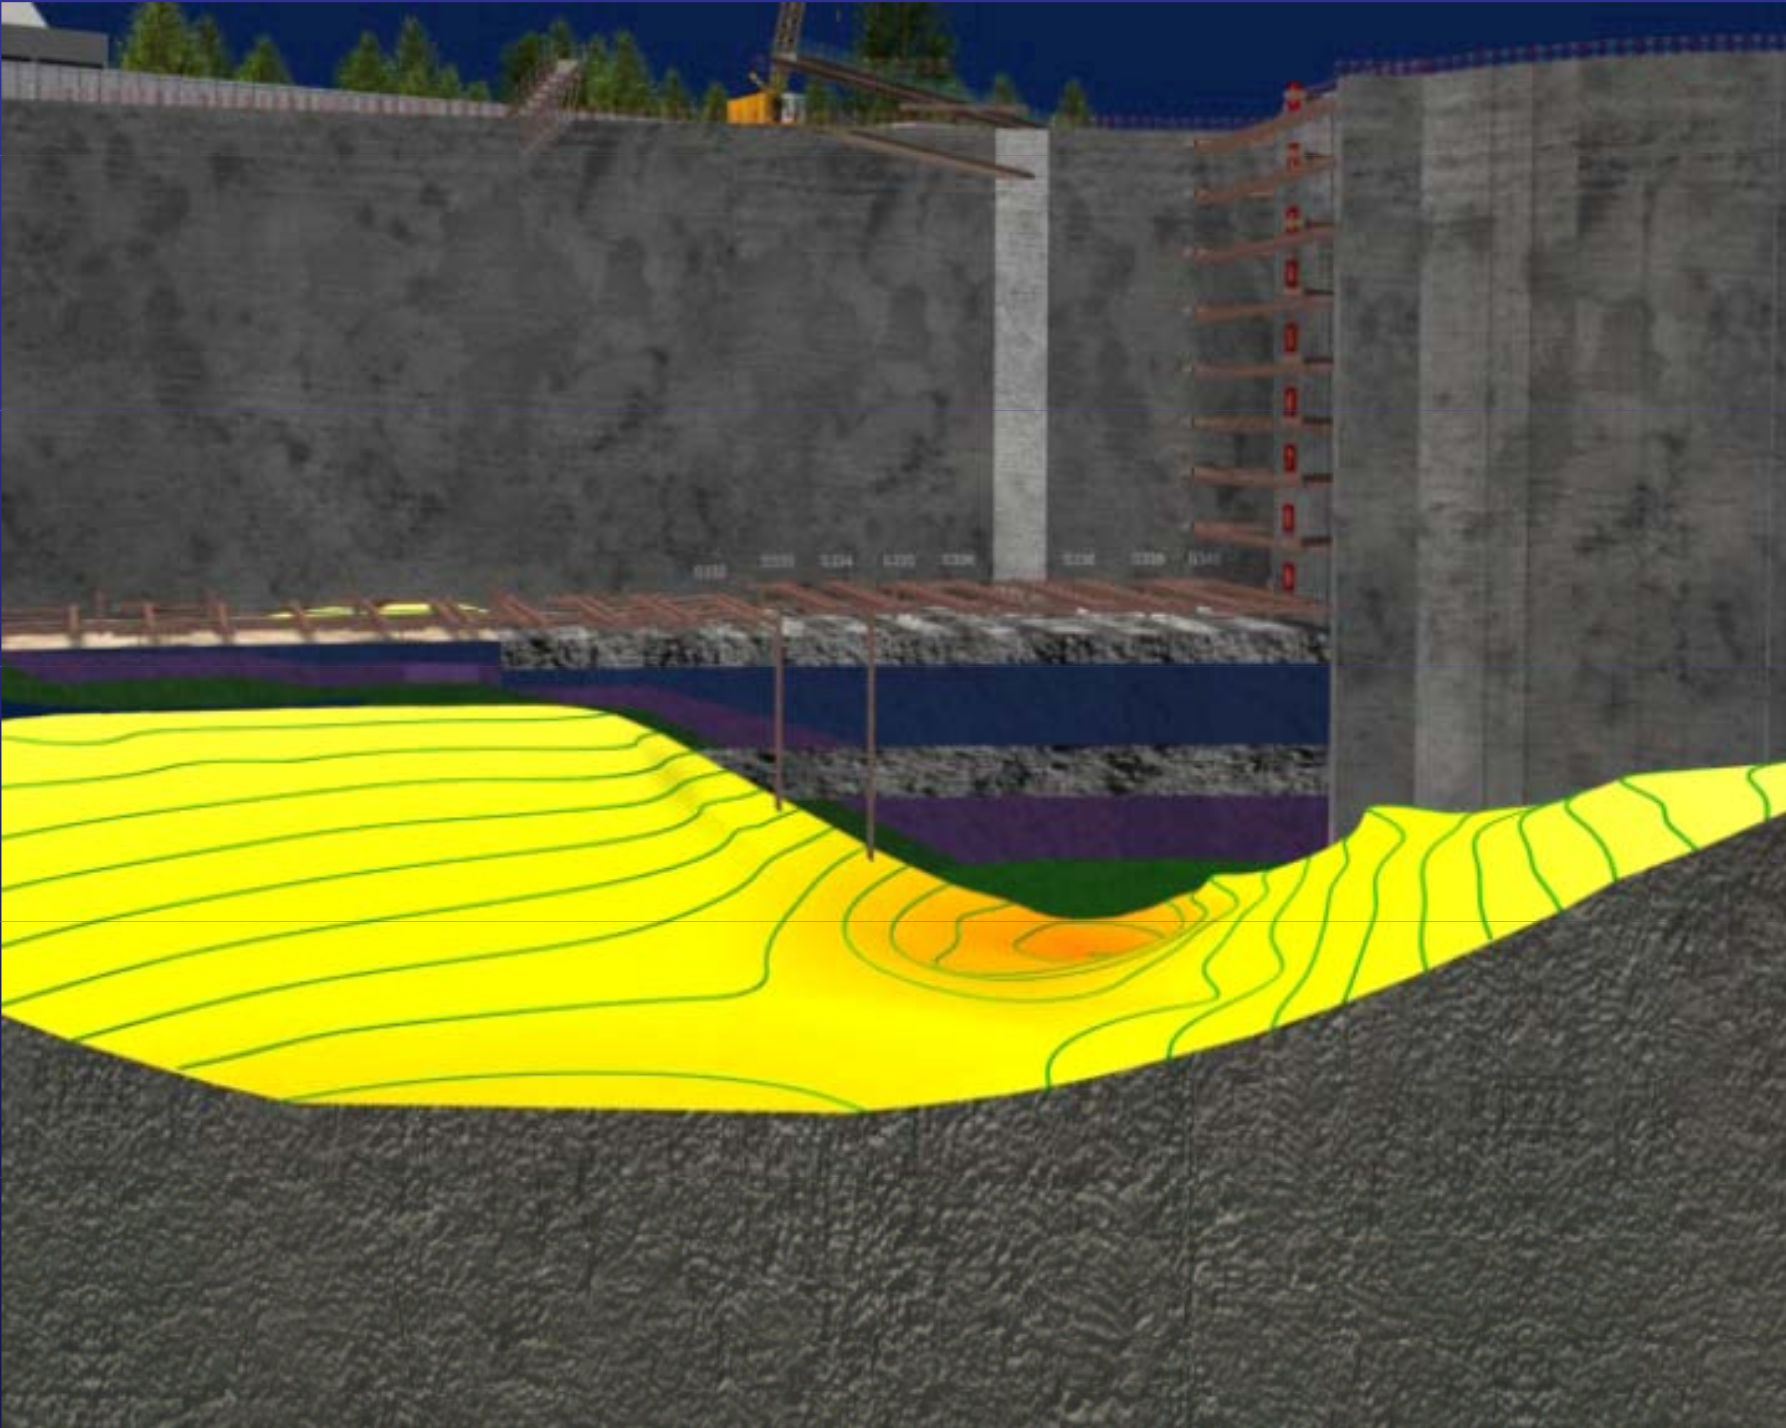
\includegraphics[width=0.8\textwidth]{figs/excavation-10-struts-jgp.png}
	\caption*{Removal of temporary jet grout}
\end{figure}
\end{frame}

%------------------------------------------------
\begin{frame}
\frametitle{On the morning of collapse}
\begin{figure}[ht]
	\centering
	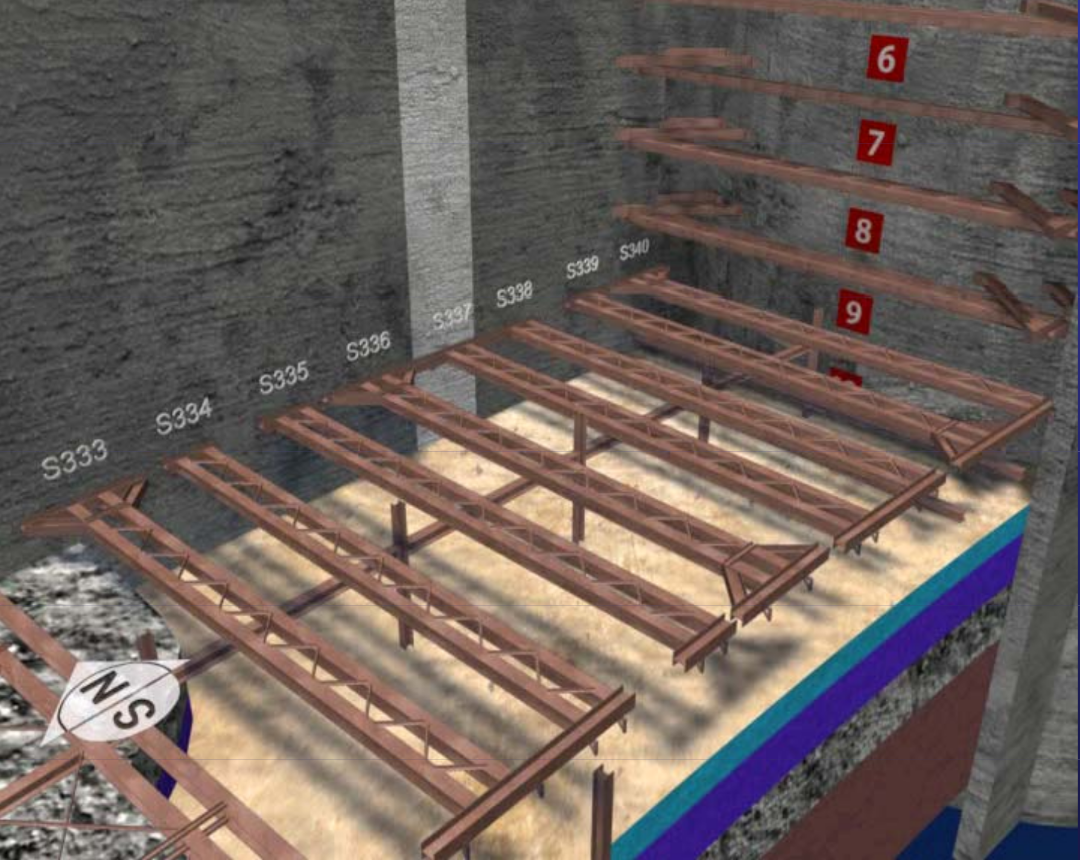
\includegraphics[width=0.8\textwidth]{figs/observation-morning-collapse.png}
\end{figure}
\end{frame}

%------------------------------------------------
\begin{frame}
\frametitle{On the morning of collapse}
\begin{figure}[ht]
	\centering
	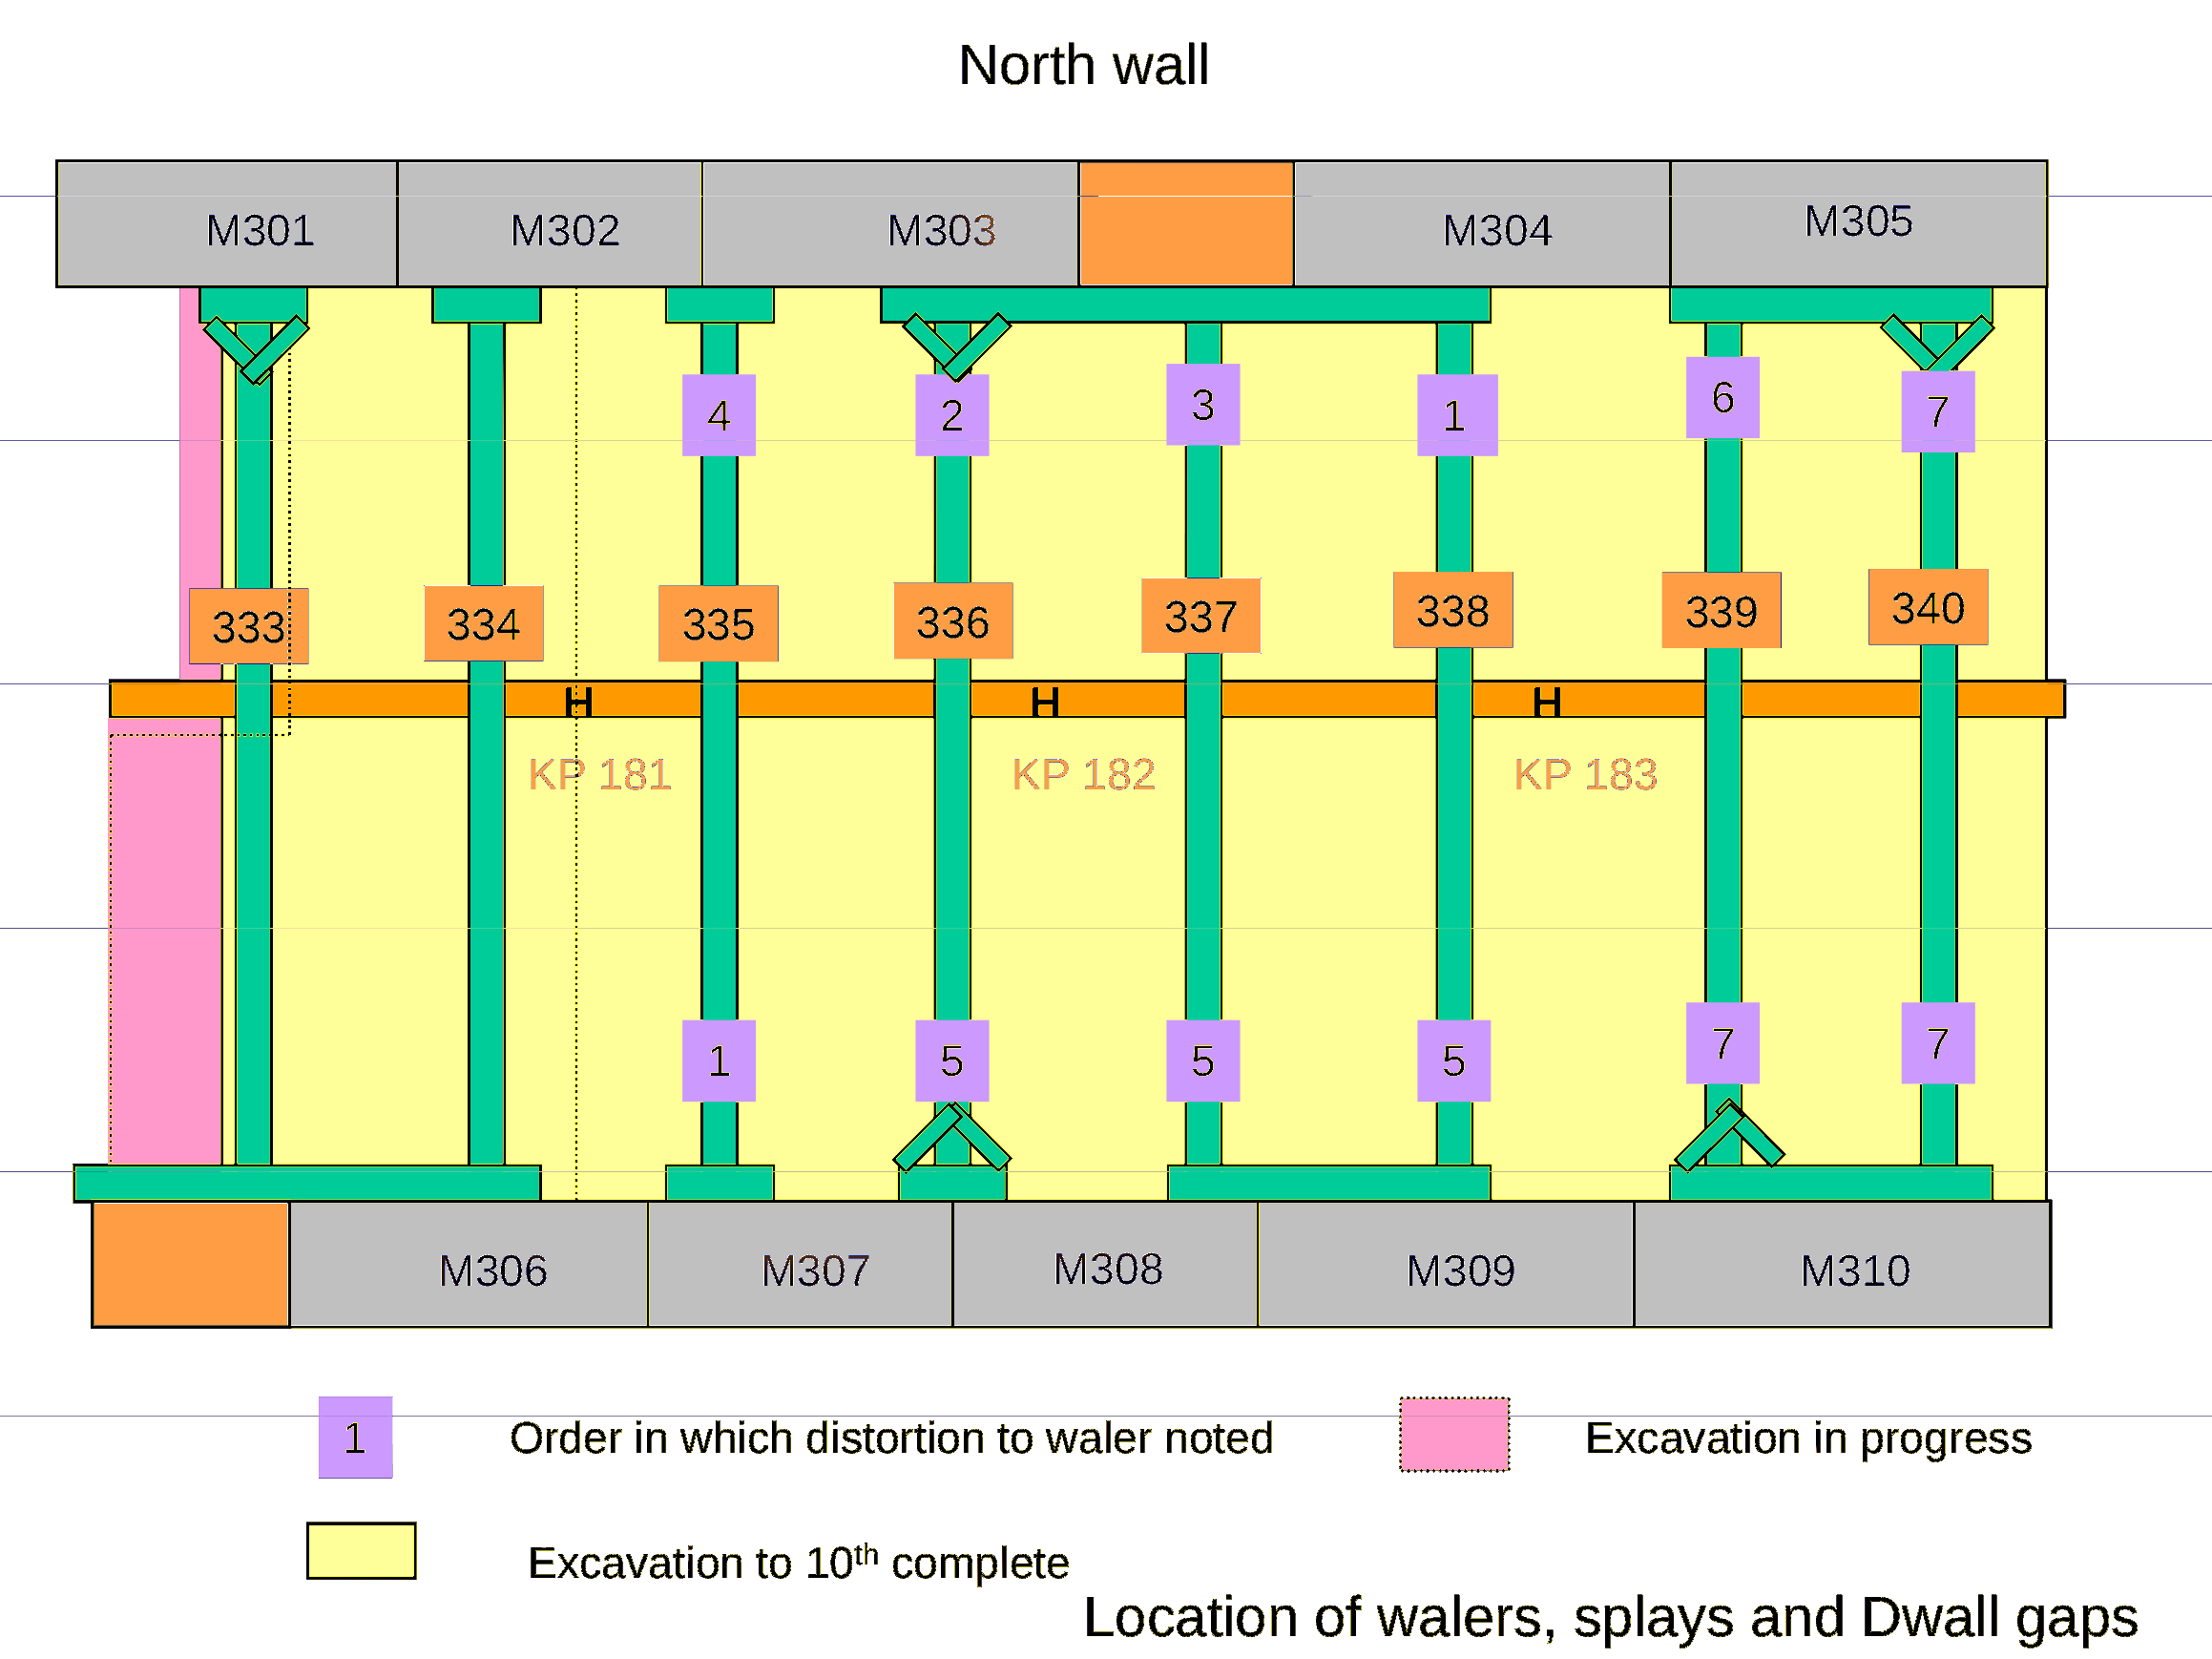
\includegraphics[width=0.8\textwidth]{figs/splays-dwall-gaps.png}
\end{figure}
\end{frame}

%------------------------------------------------
\begin{frame}
\frametitle{On the morning of collapse}
\begin{figure}[ht]
	\centering
	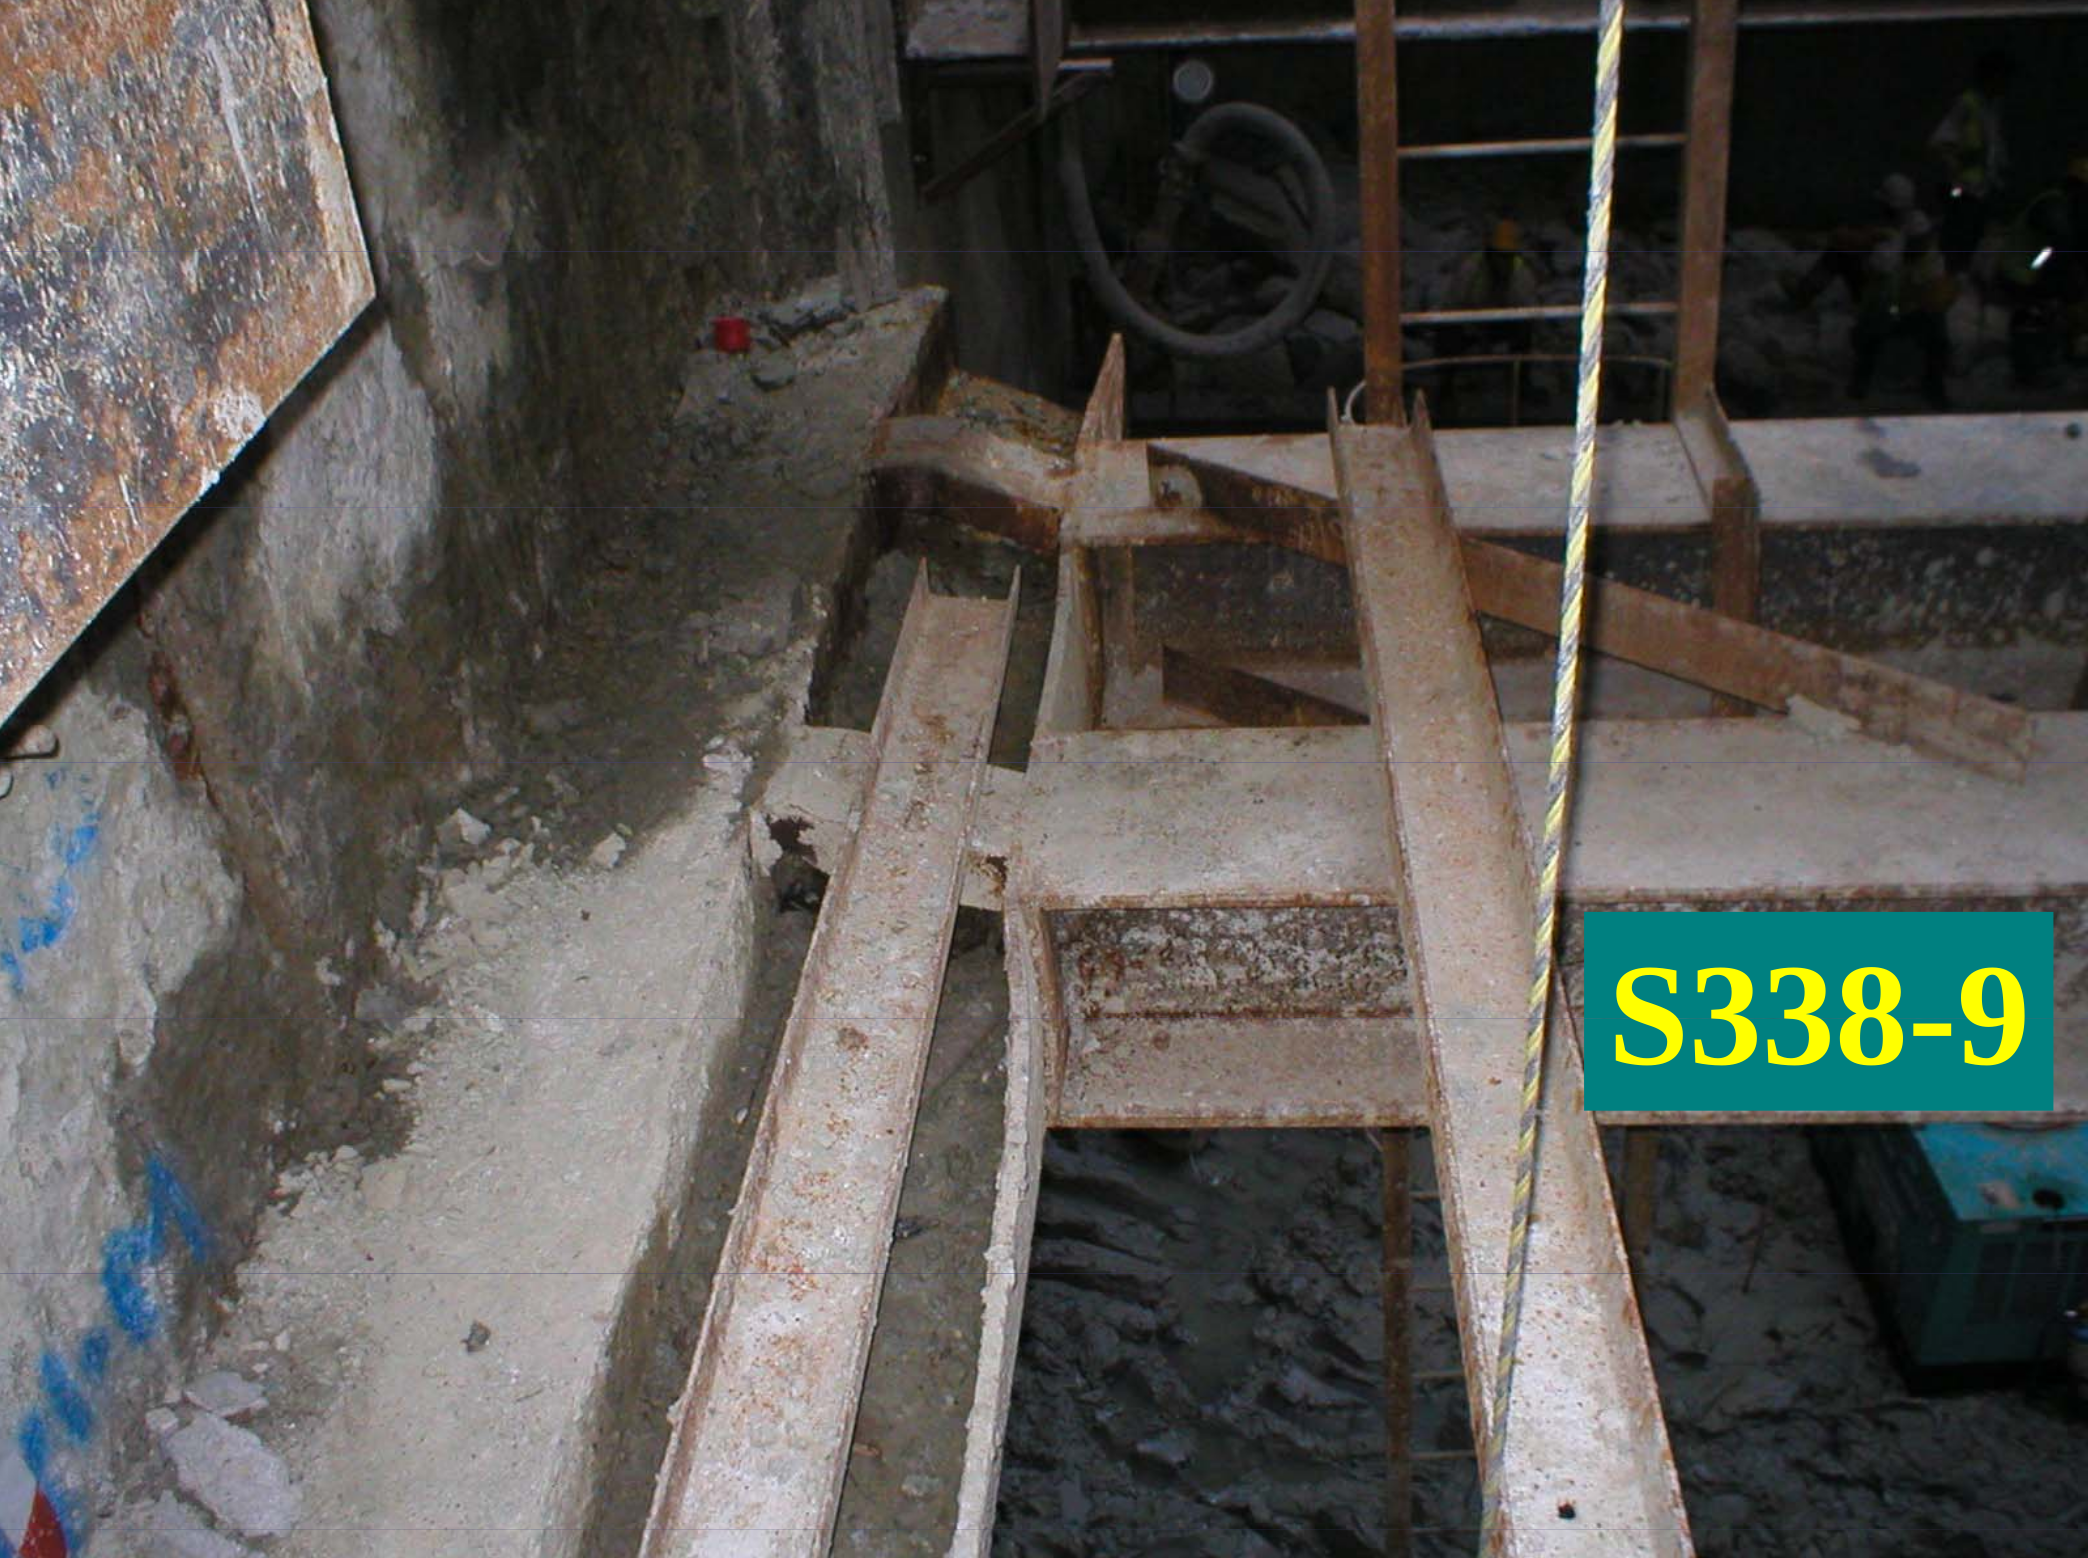
\includegraphics[width=0.8\textwidth]{figs/strut-338.png}
	\caption*{Strut 338 North side}
\end{figure}
\end{frame}

%------------------------------------------------
\begin{frame}
\frametitle{On the morning of collapse}
\begin{figure}[ht]
	\centering
	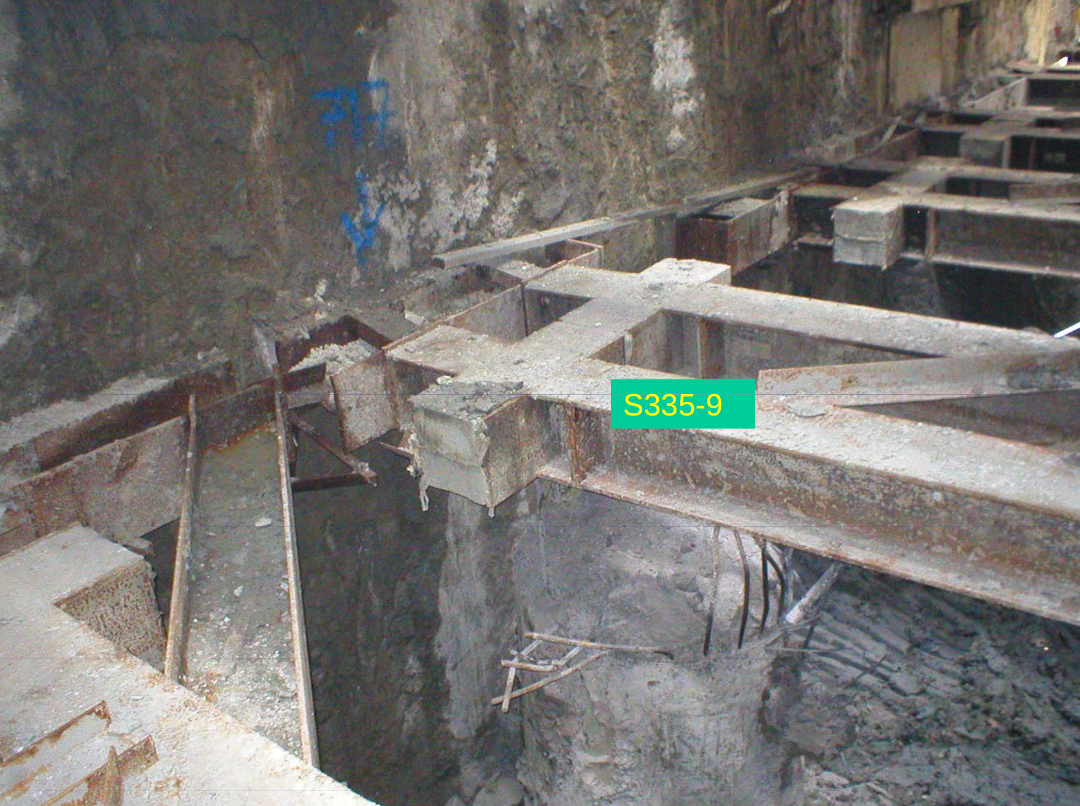
\includegraphics[width=0.8\textwidth]{figs/strut-335-south.png}
	\caption*{Strut 335 Sorth side}
\end{figure}
\end{frame}

%------------------------------------------------
\begin{frame}
\frametitle{Hours before collapse}
\begin{figure}[ht]
	\centering
	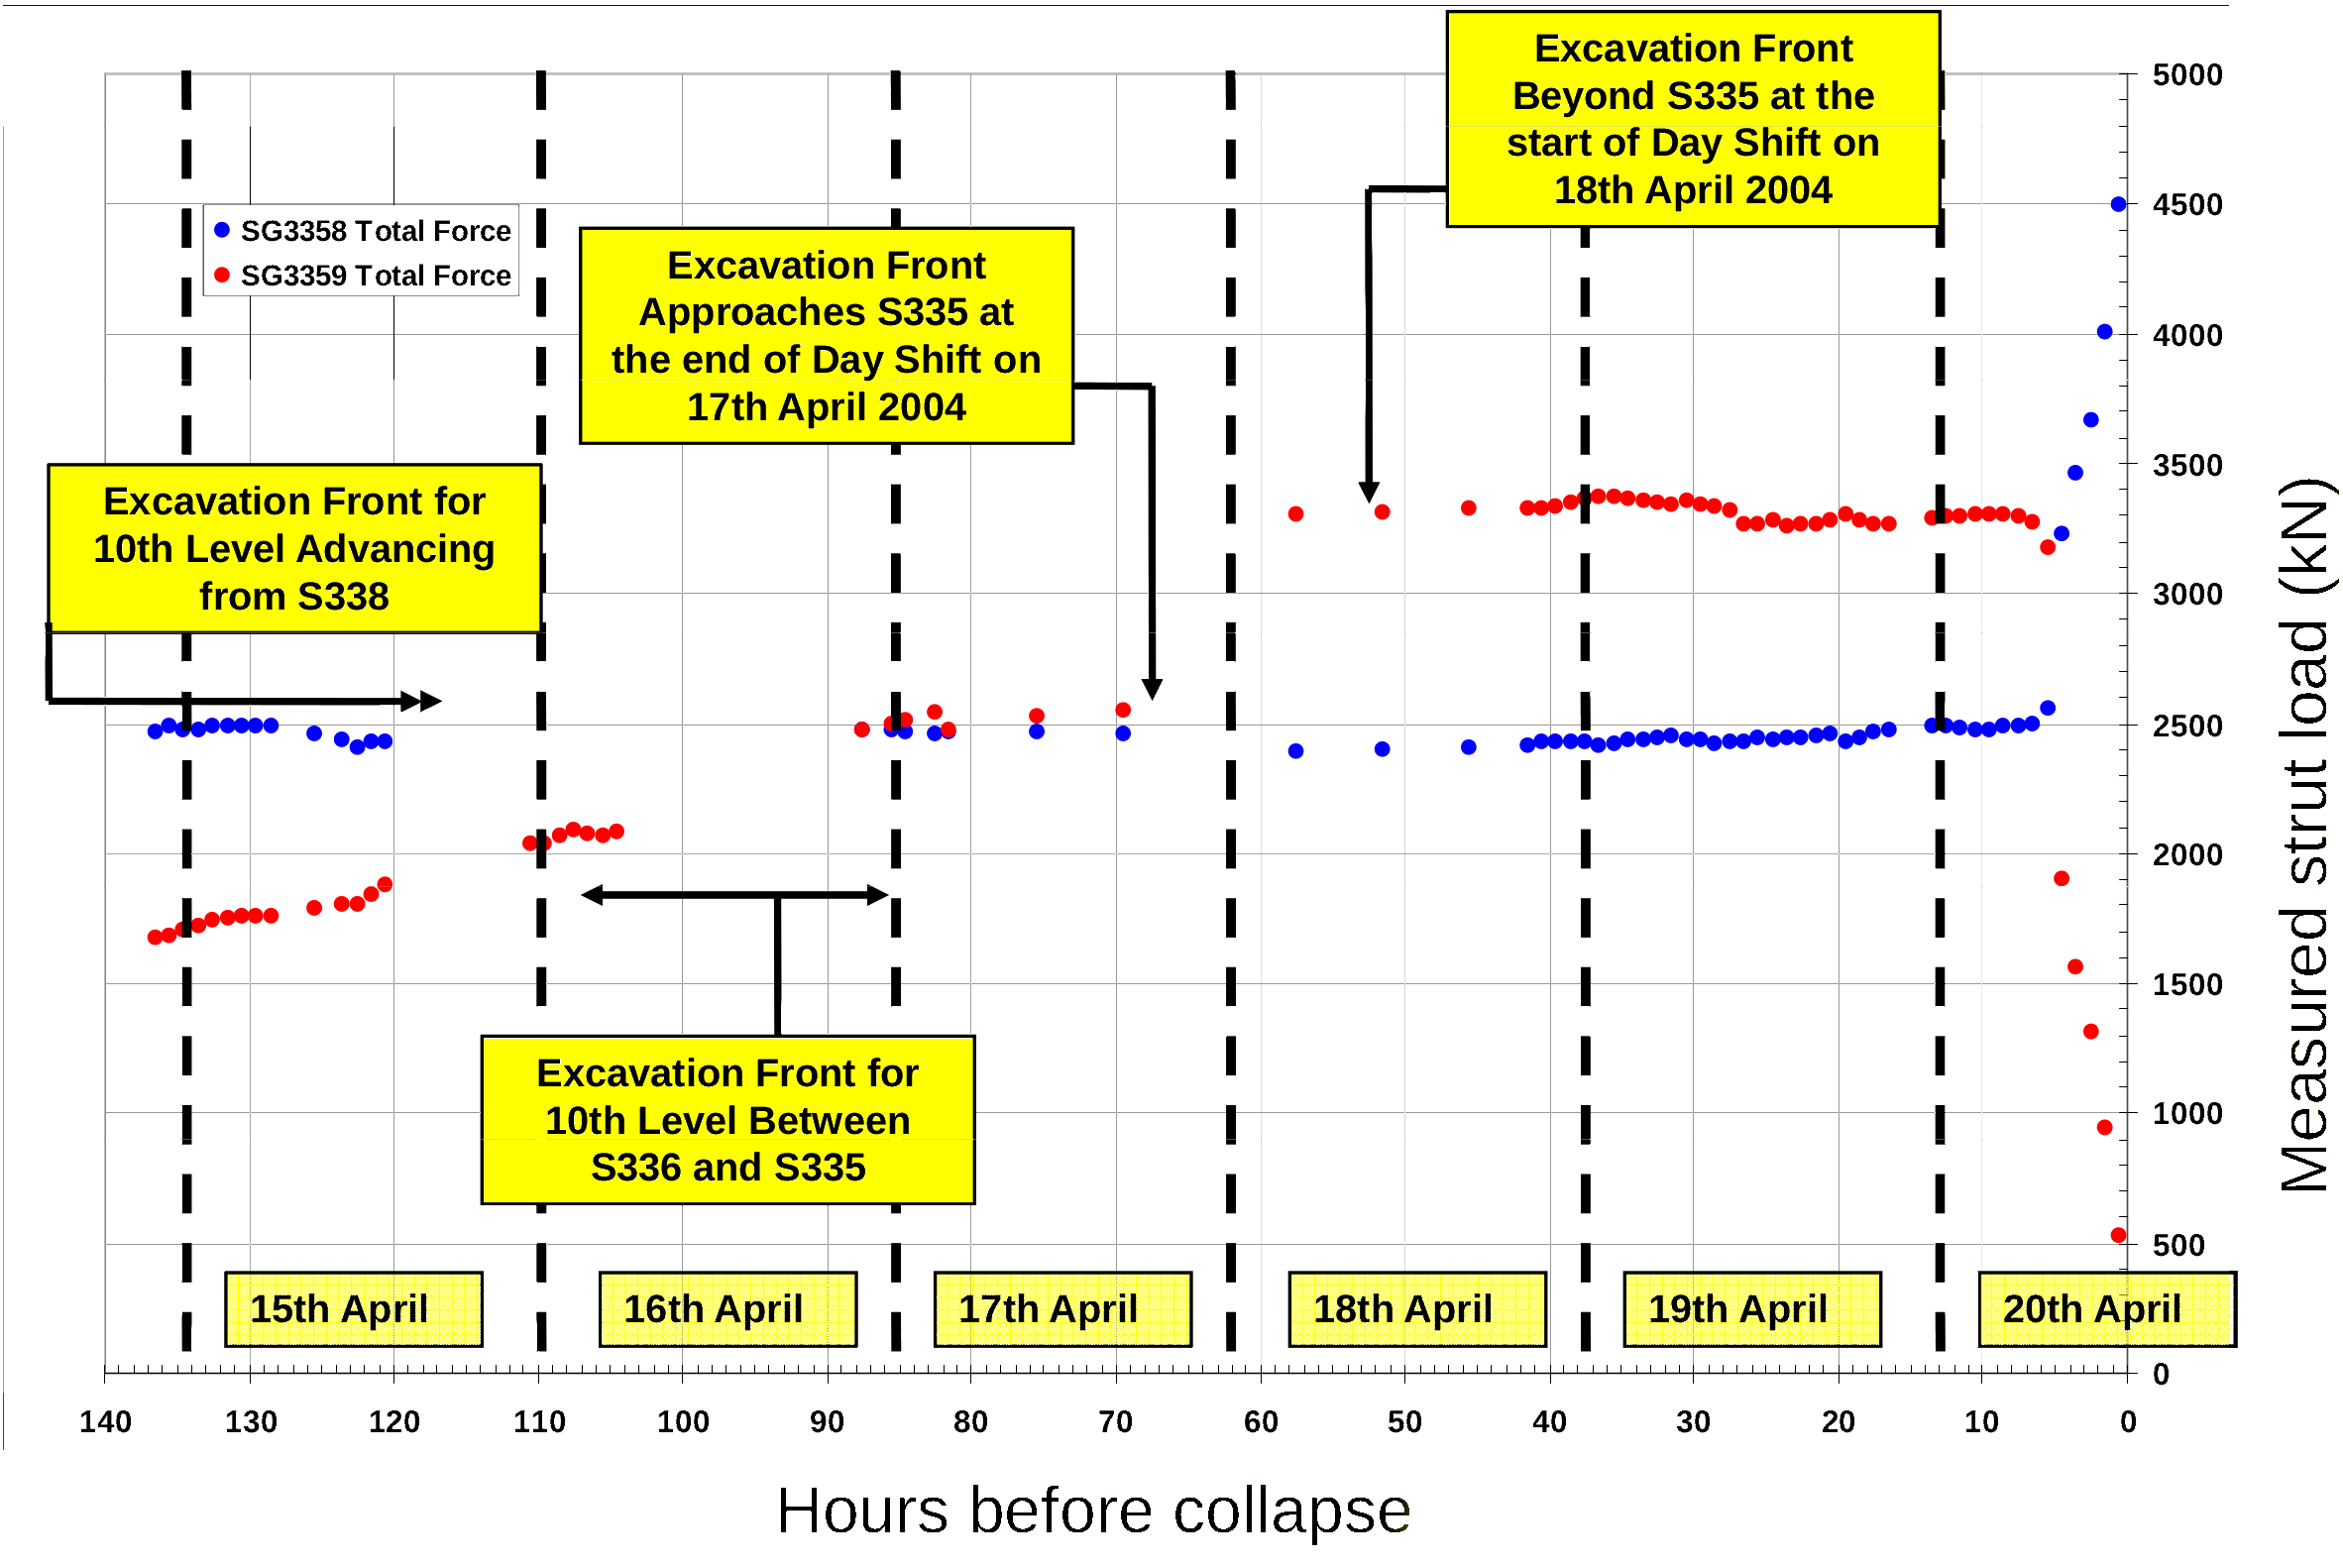
\includegraphics[width=0.8\textwidth]{figs/strut-load-before-collapse.png}
\end{figure}
\end{frame}

%------------------------------------------------
\begin{frame}
\frametitle{Hours before collapse}
\begin{figure}[ht]
	\centering
	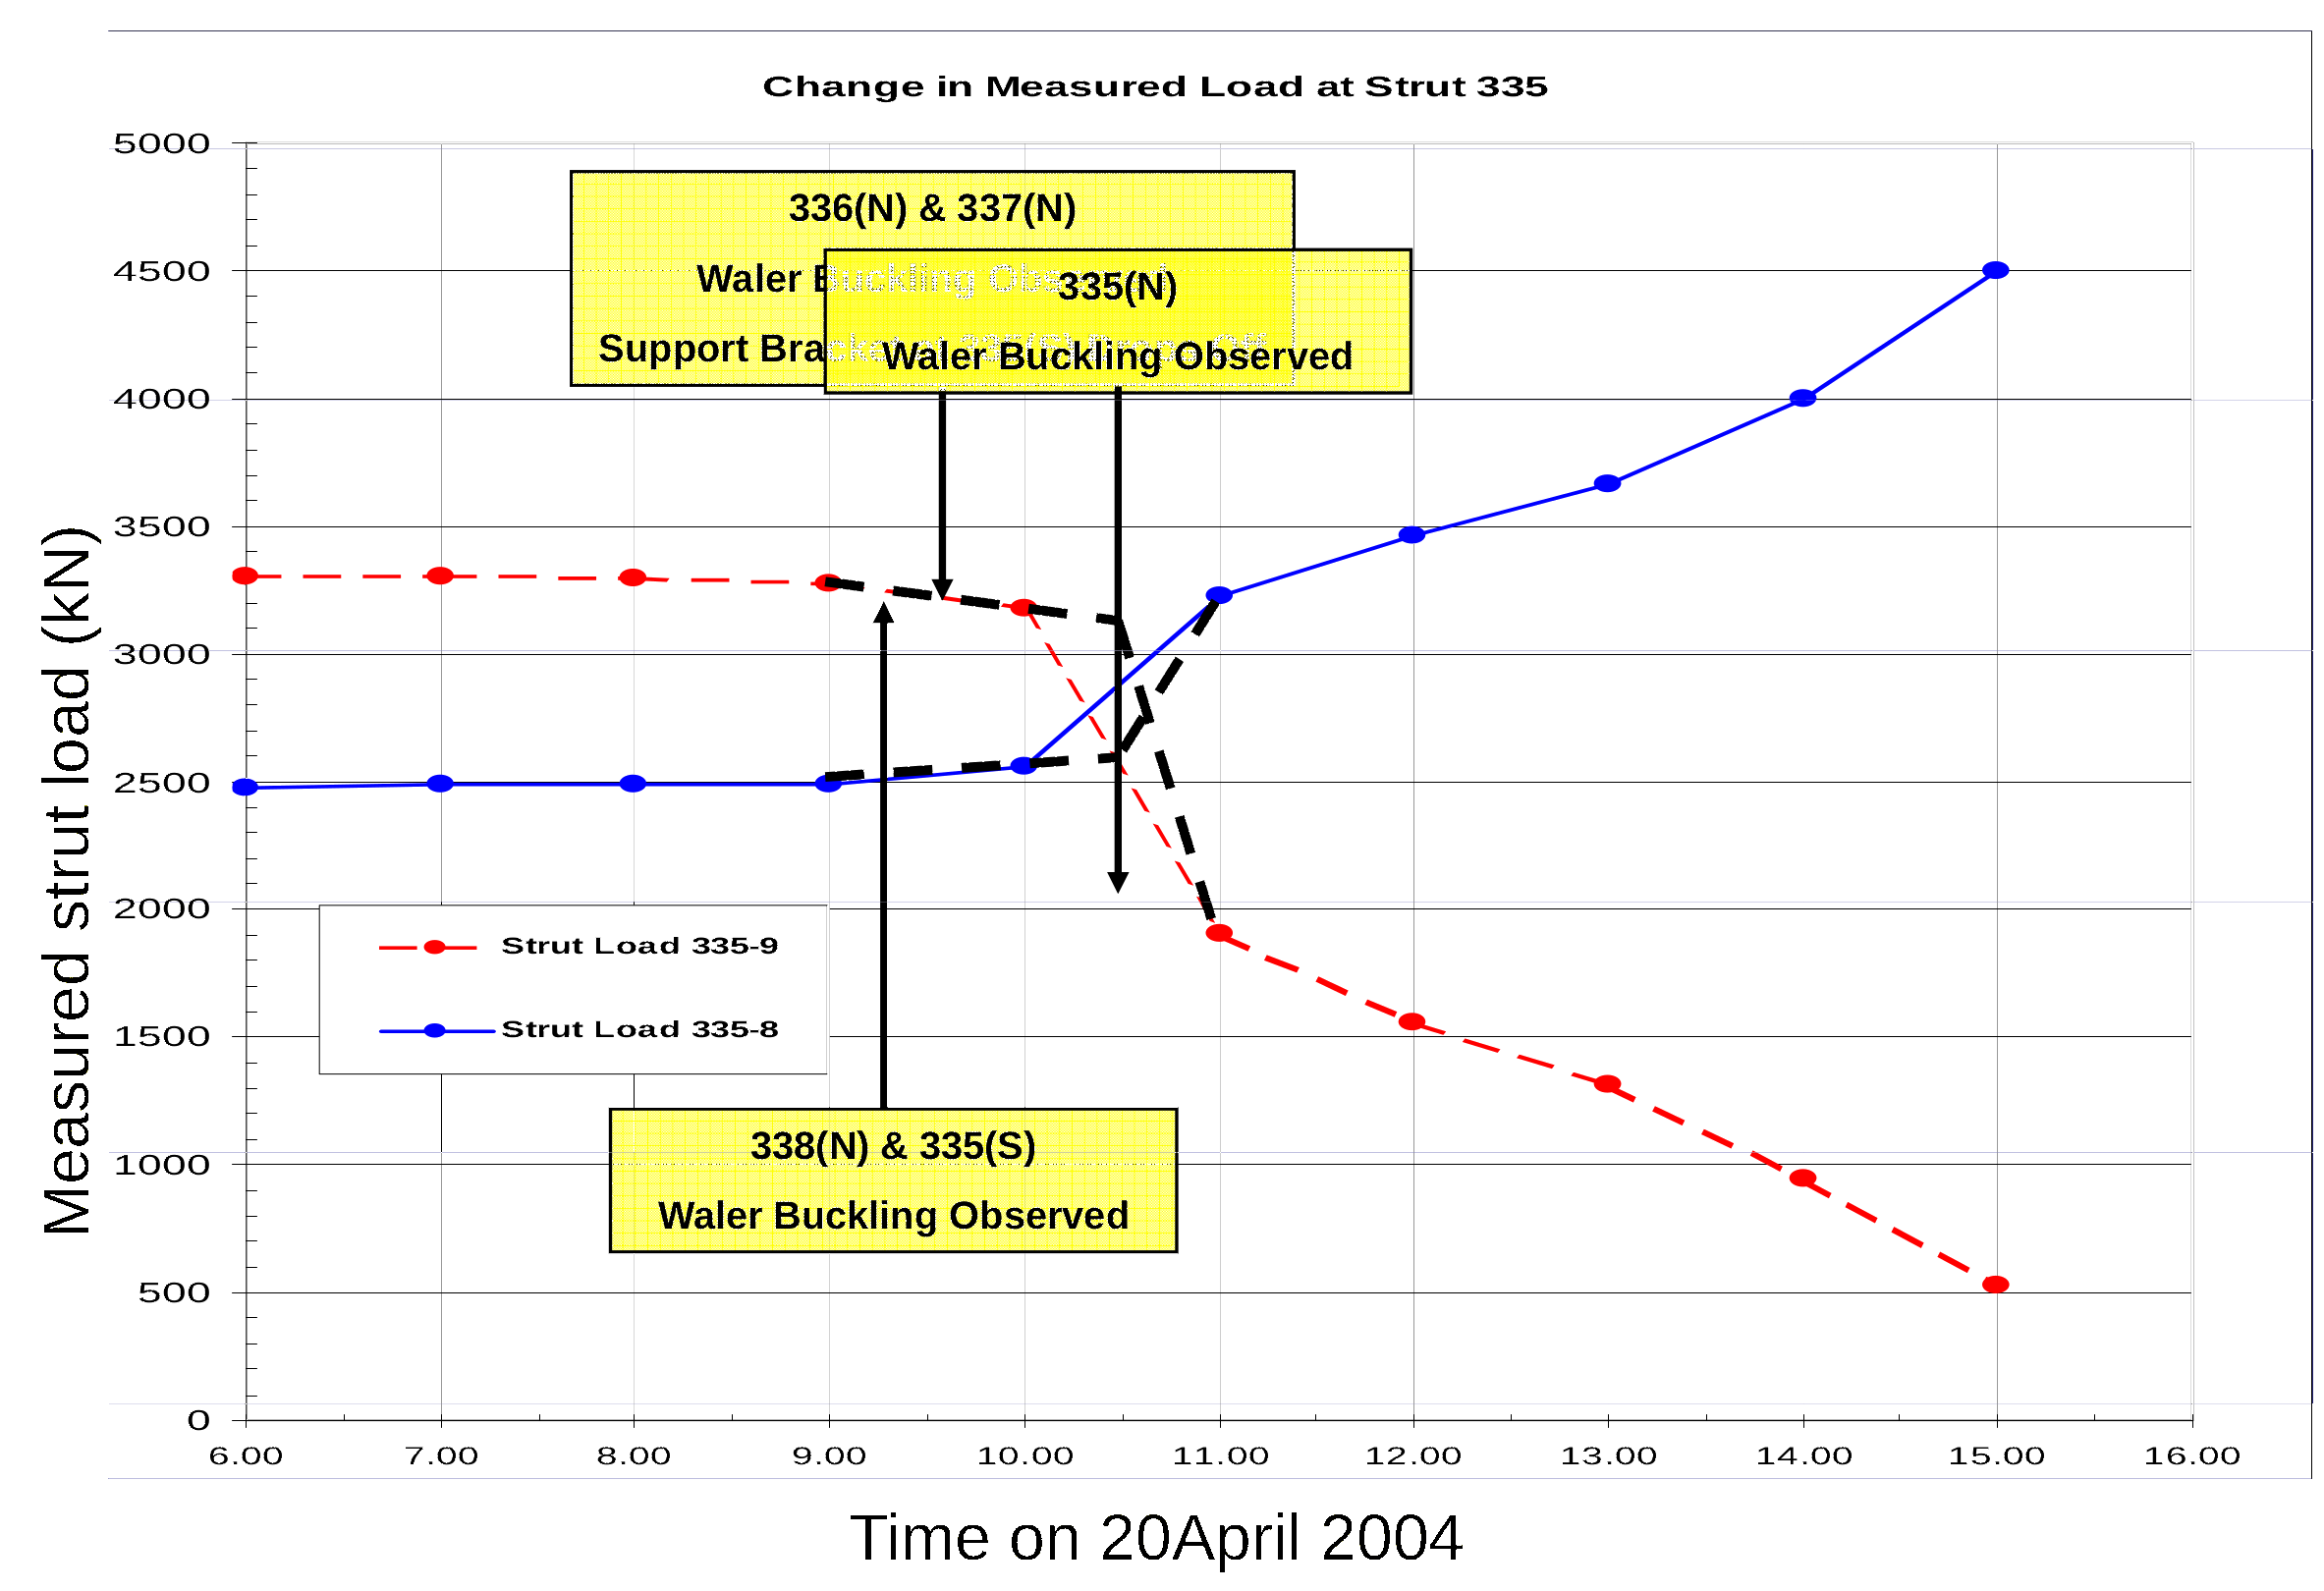
\includegraphics[width=0.8\textwidth]{figs/struct-load-time.png}
\end{figure}
\end{frame}

\note{In the meanwhile the excavation progressed to about the 10th level of struts. The temporary layer of jet grout piles below the 10th level which was constructed to add to the stability of the excavation was now removed to finish the excavation of the tunnel. Two more temporary struts were added to stabilize the excavation. By 19th April the excavation of the tunnel was completed and the last bit of the tunnel section connecting it with the other section of the tunnel was cut out and the tunnels were connected. On the day of the collapse the 20th of April at around 8:00 am the workers at the site heard sounds from the multi-level strut system. The strange sounds were investigated by the senior engineers of the contractor and they found that a lot of the waler-strut connections had yielded. They immediately instructed everyone to leave the worksite.}
	
\note{ By noon engineers from the owner’s side were also present at the worksite and they along with the contractor’s engineers decided to pour concrete at the 9th level of the strut to stabilize the excavation and prevent it from caving in. By 3:30 pm the temporary system gave away and the tunnel had caved in.\\
	
	The trends were consistent with there being yielding of the 0th level strut-waler connection when the exvavation passed beneath but with no further significant changes in load in eiter the 9th or 8th level struts until the collapse was initiated.
}
%------------------------------------------------
\begin{frame}
\frametitle{Leading up to the collapse: Inclinometer}
\begin{figure}[ht]
	\centering
	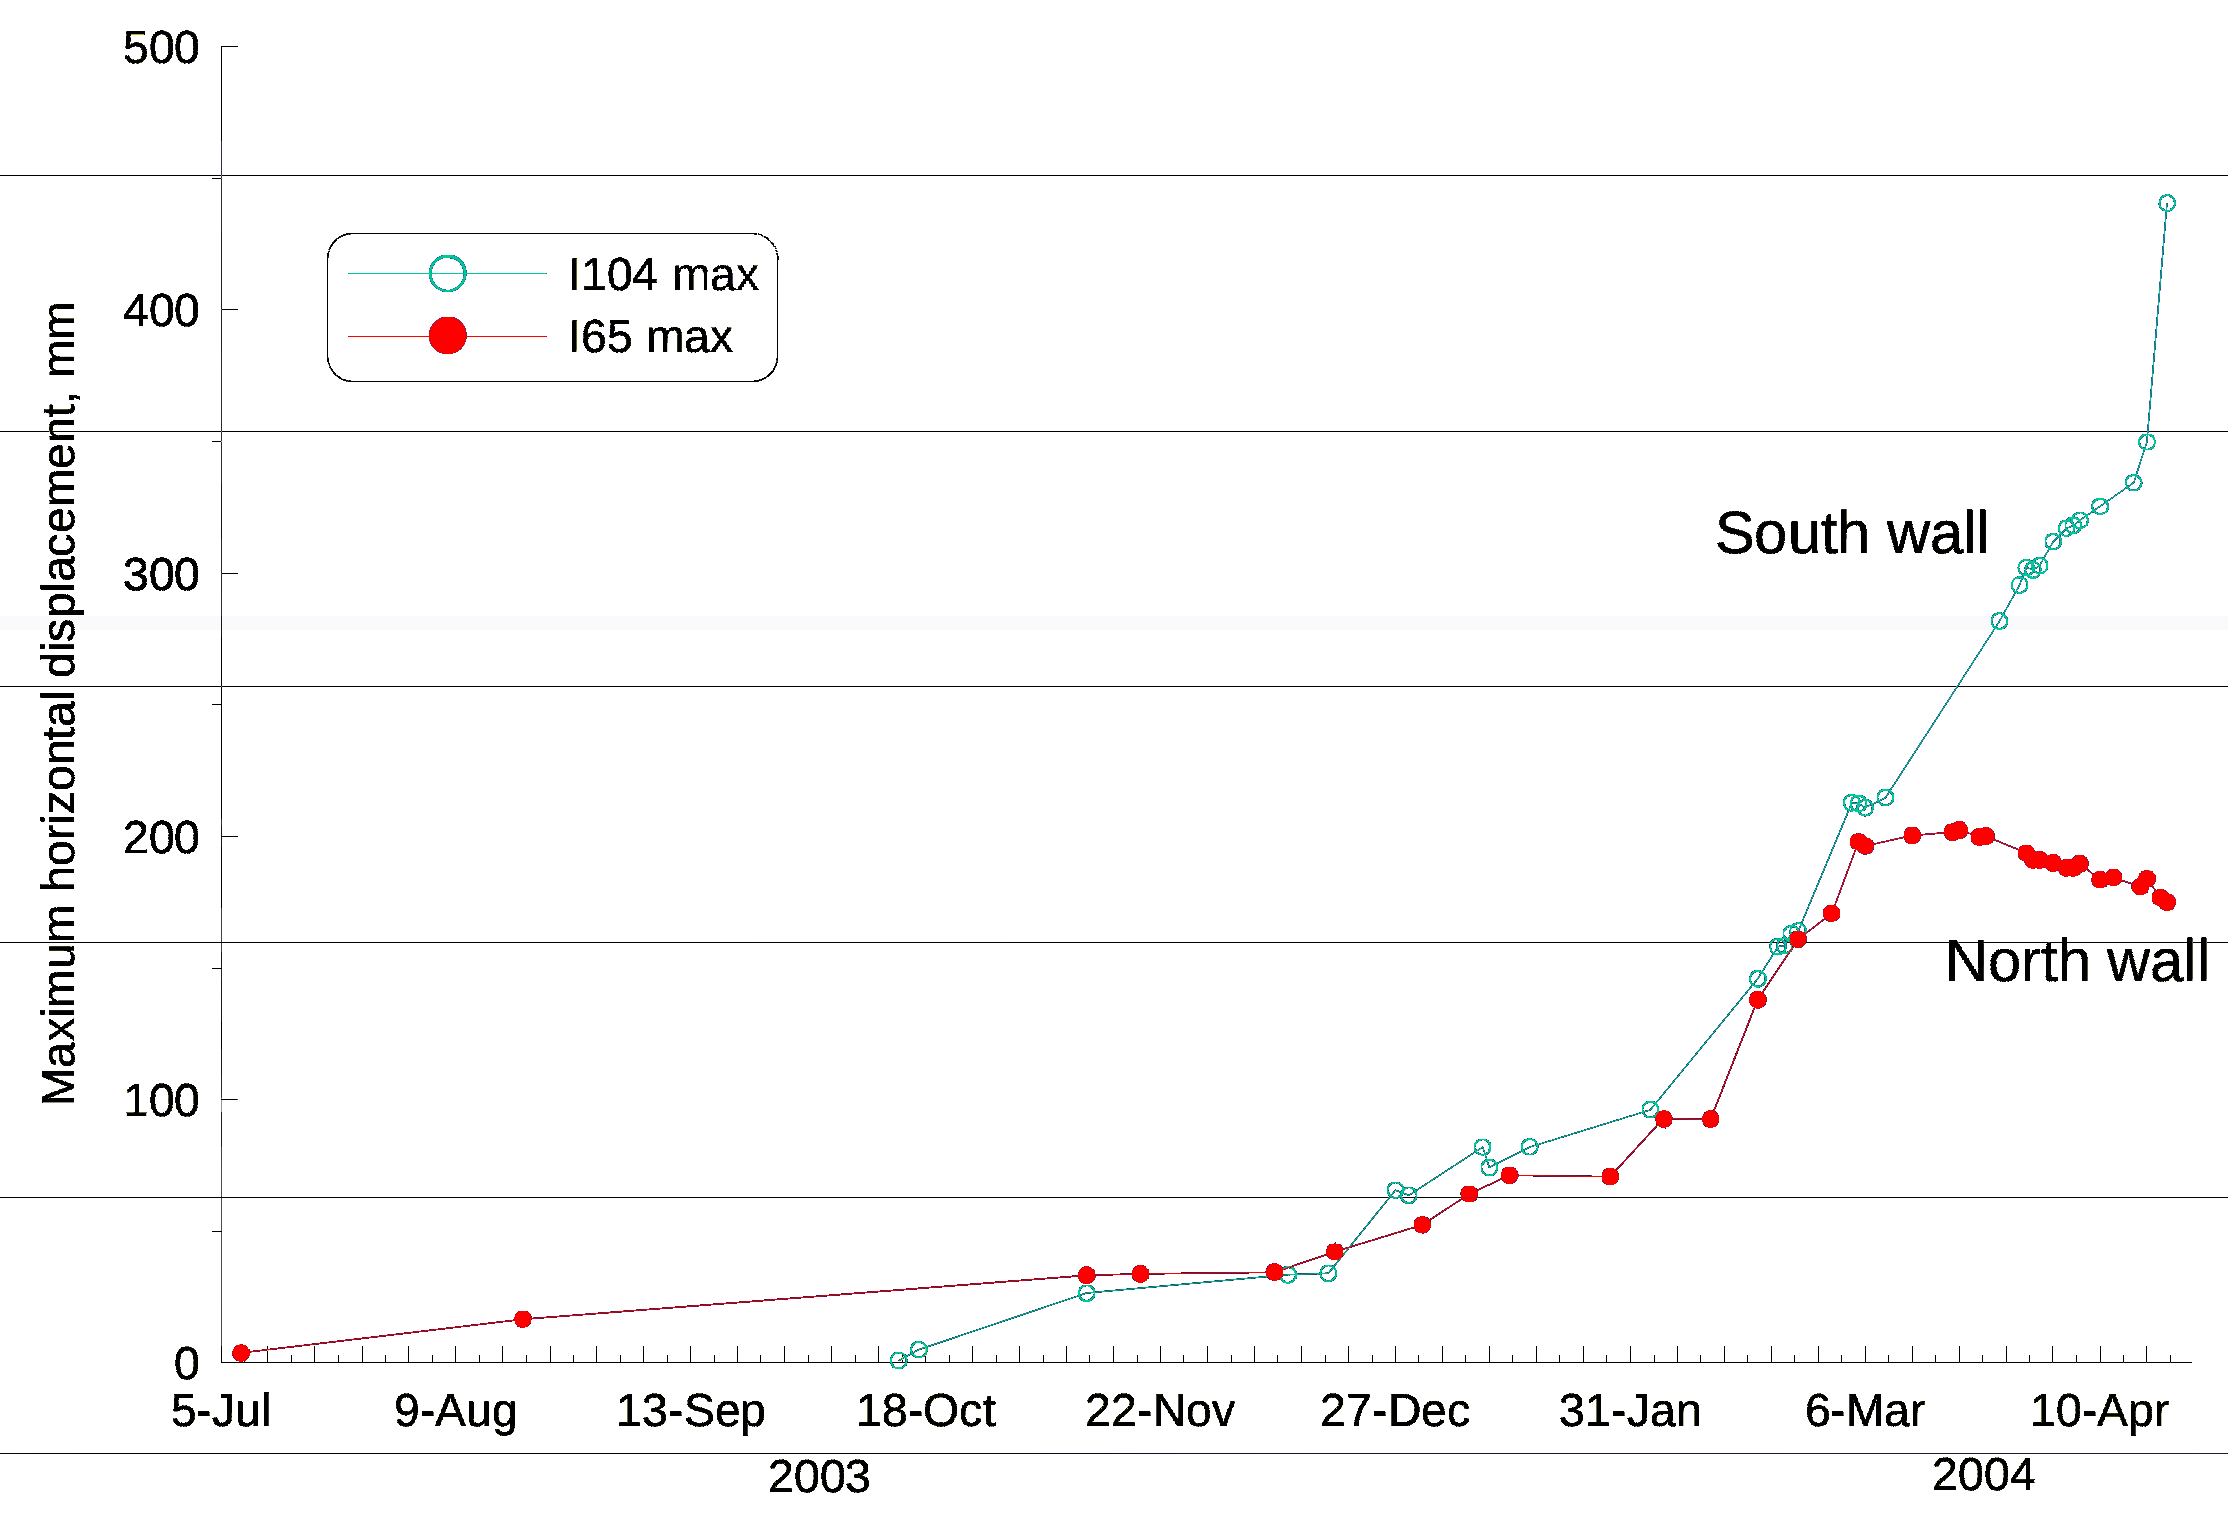
\includegraphics[width=0.8\textwidth]{figs/inclinometer.png}
\end{figure}
\end{frame}


%------------------------------------------------
\begin{frame}
\frametitle{Leading up to the collapse: Wall displacements}
\begin{figure}[ht]
	\centering
	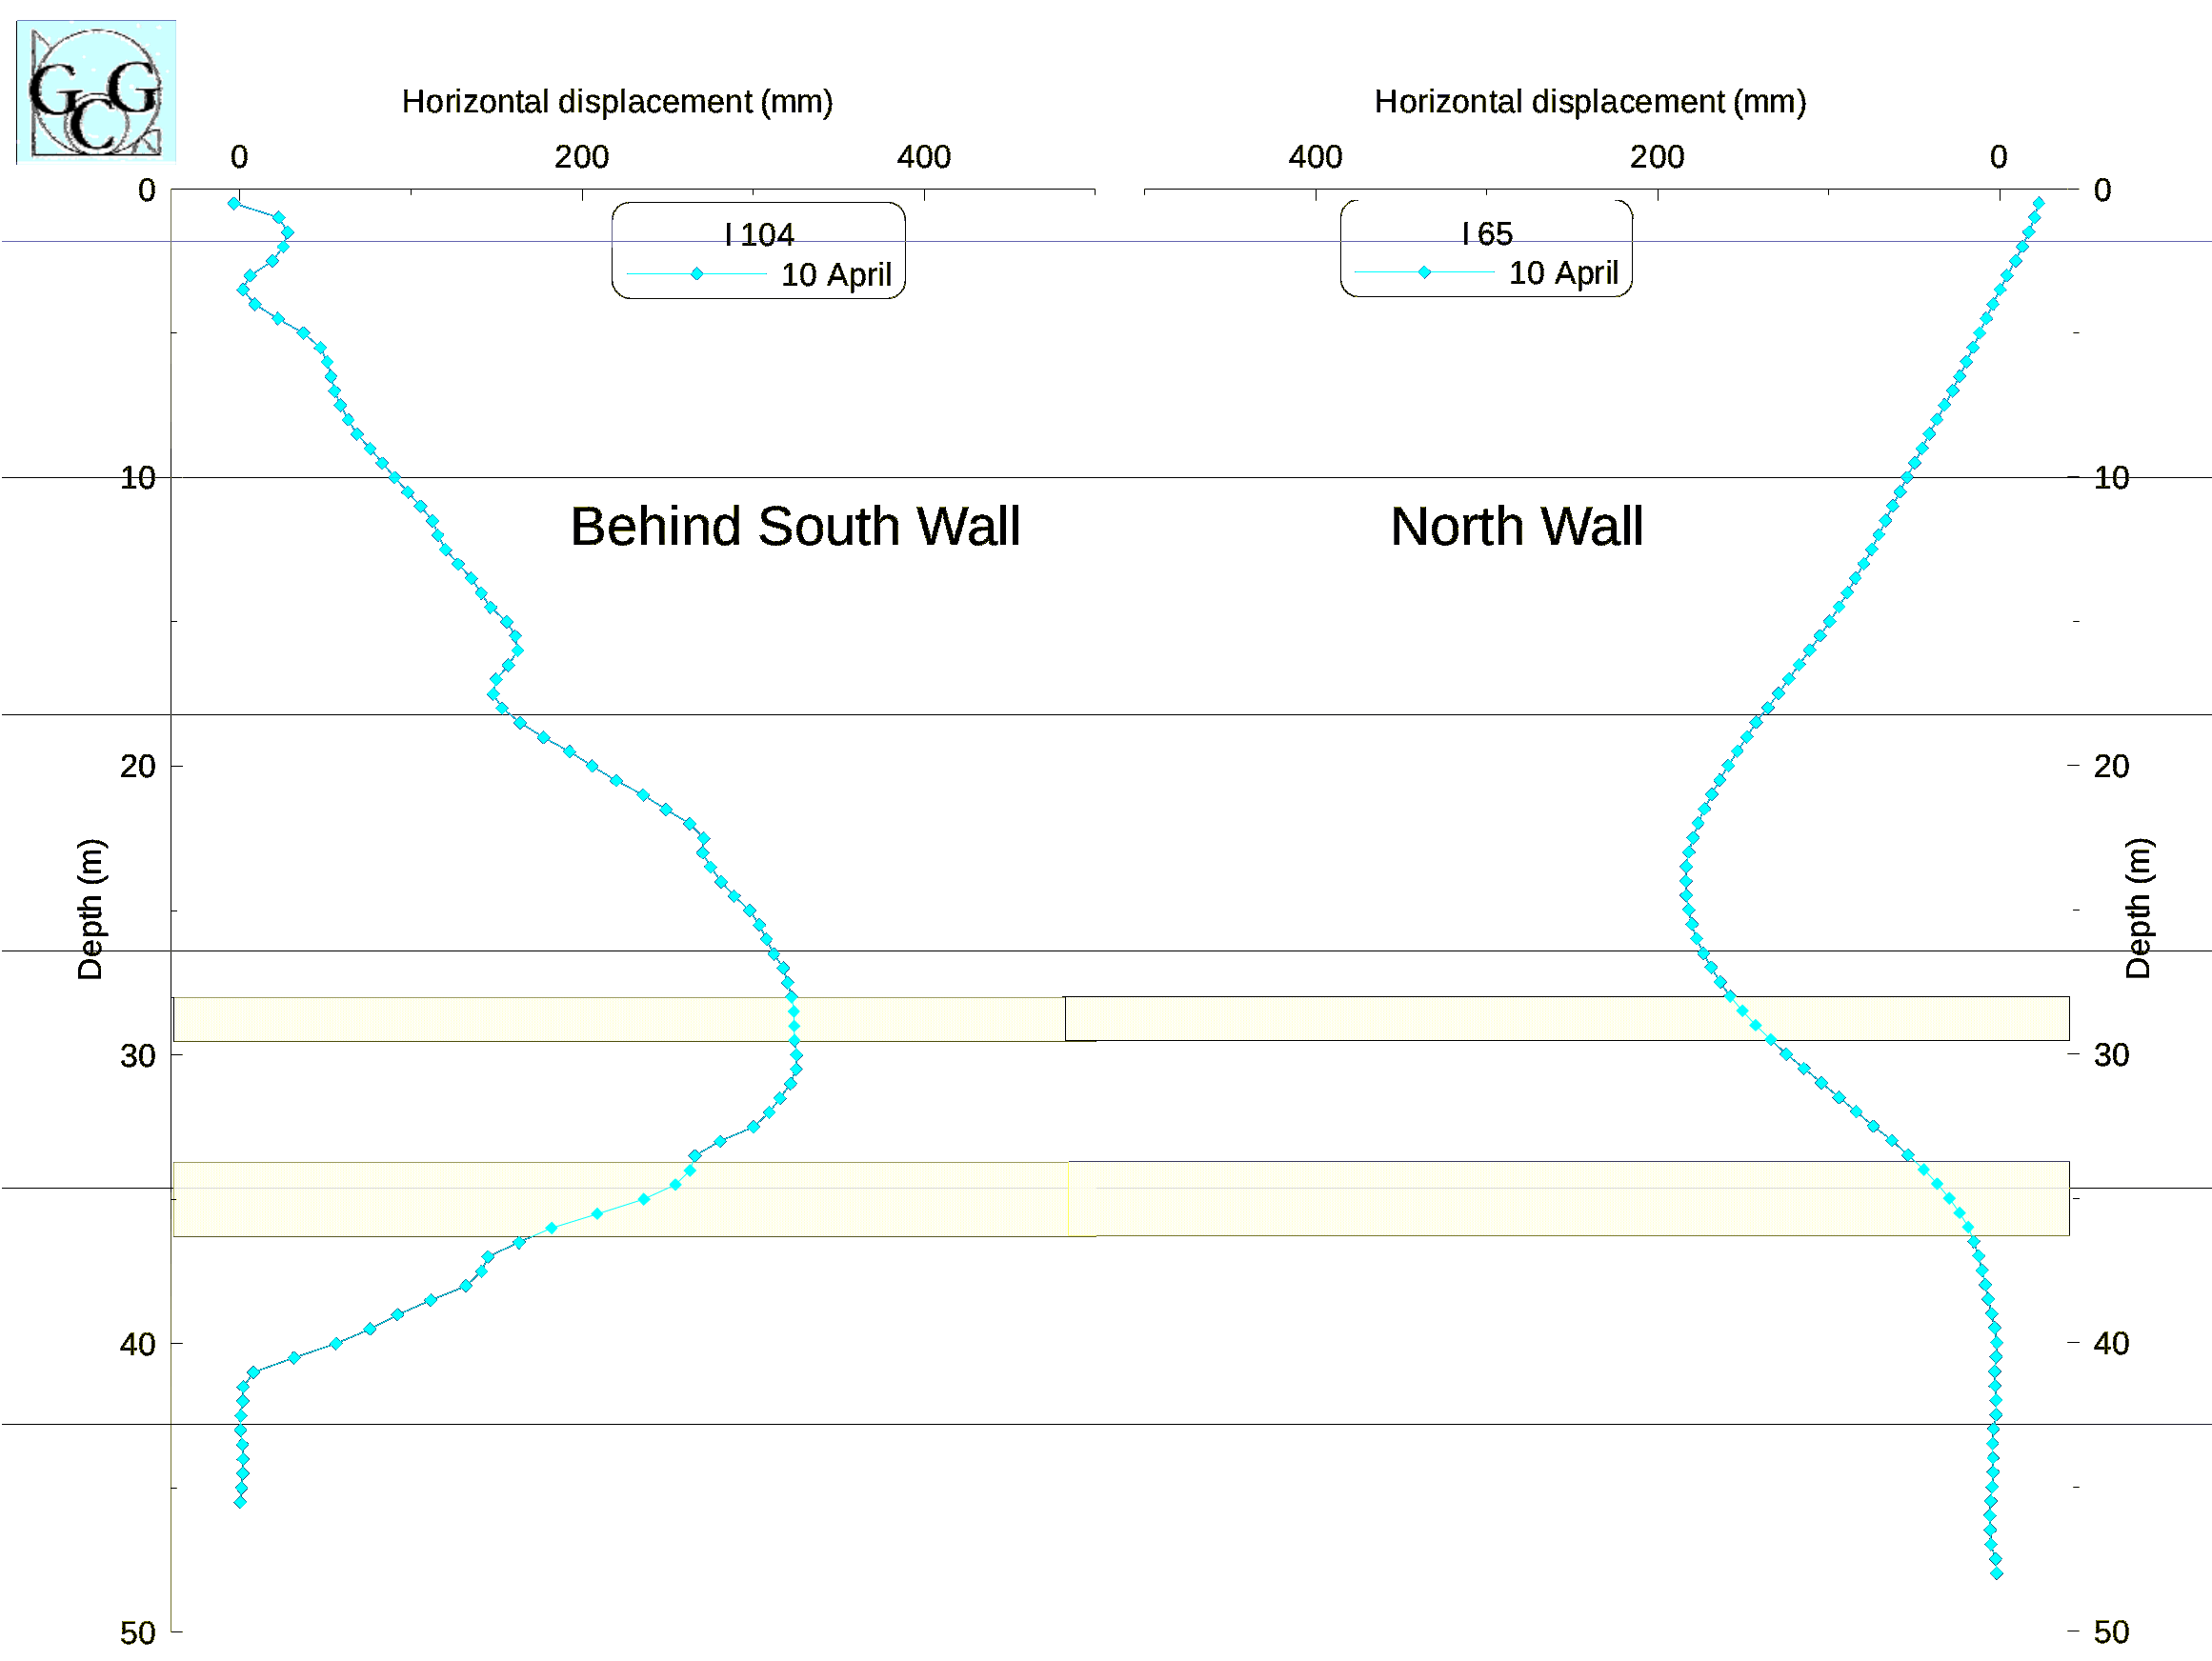
\includegraphics[width=0.8\textwidth]{figs/disp1.png}
\end{figure}
\end{frame}


%------------------------------------------------
\begin{frame}
\frametitle{Leading up to the collapse: Wall displacements}
\begin{figure}[ht]
\centering
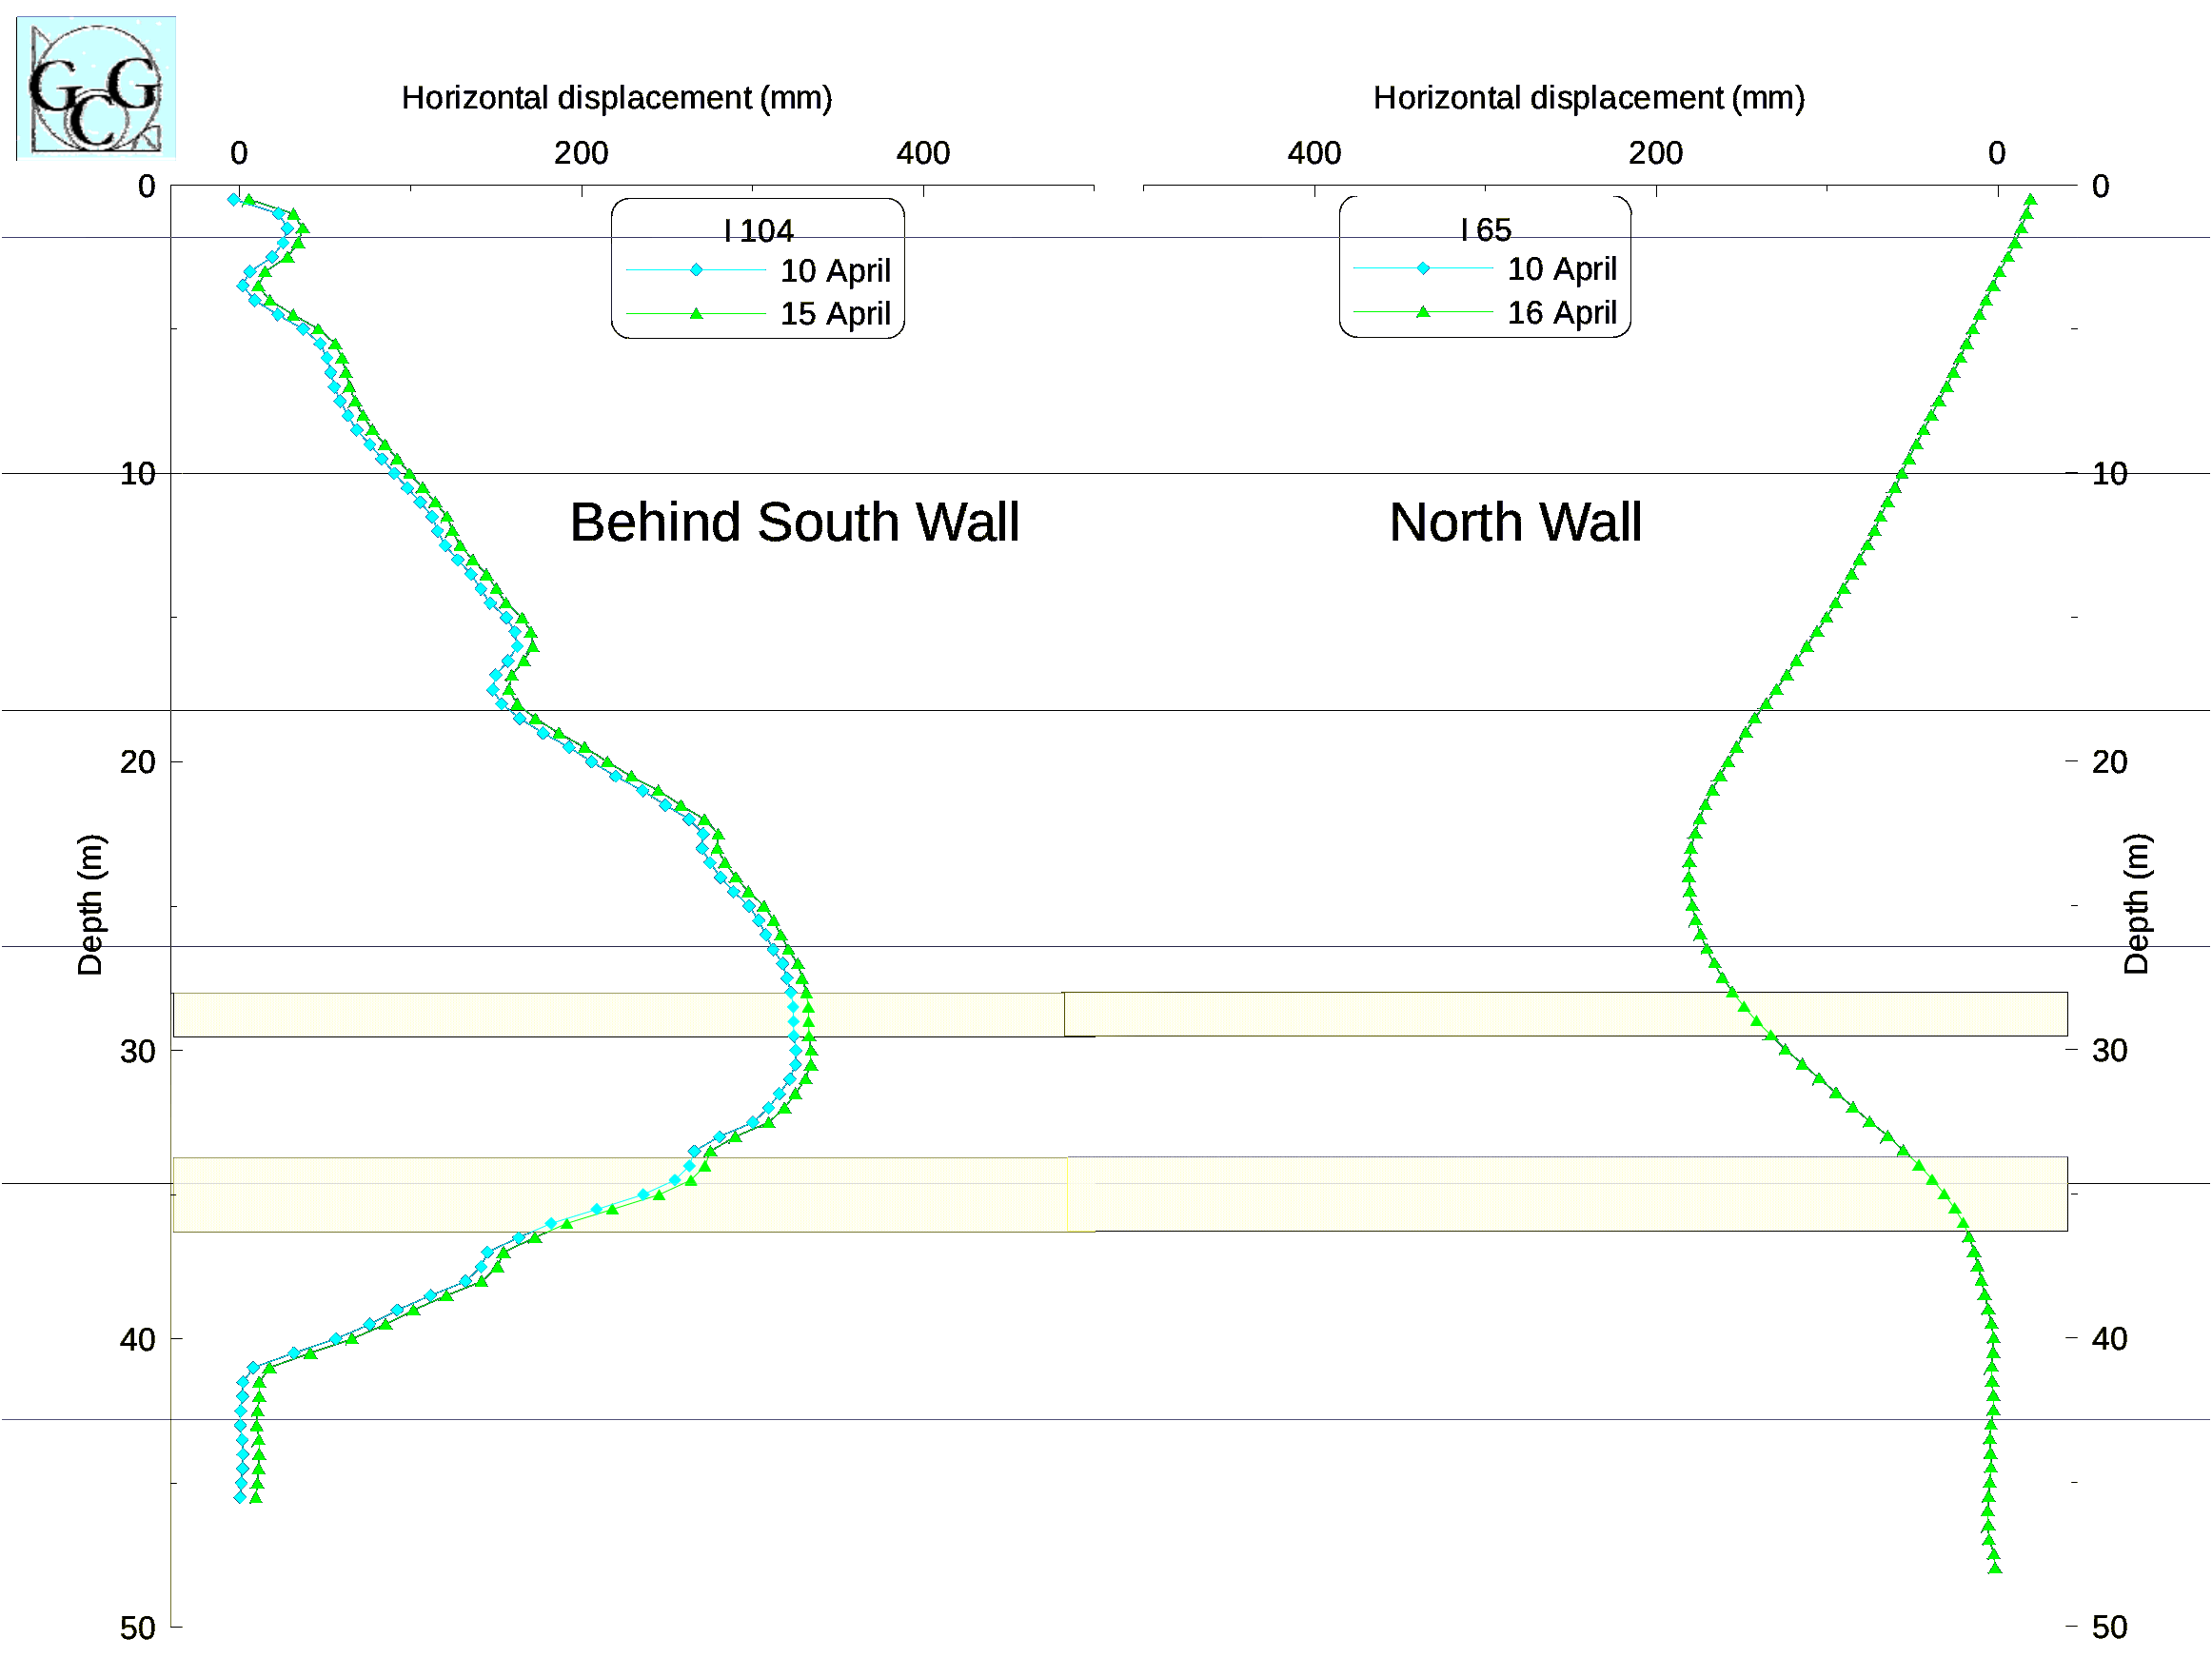
\includegraphics[width=0.8\textwidth]{figs/disp2.png}
\end{figure}
\end{frame}

%------------------------------------------------
\begin{frame}
\frametitle{Leading up to the collapse: Wall displacements}
\begin{figure}[ht]
	\centering
	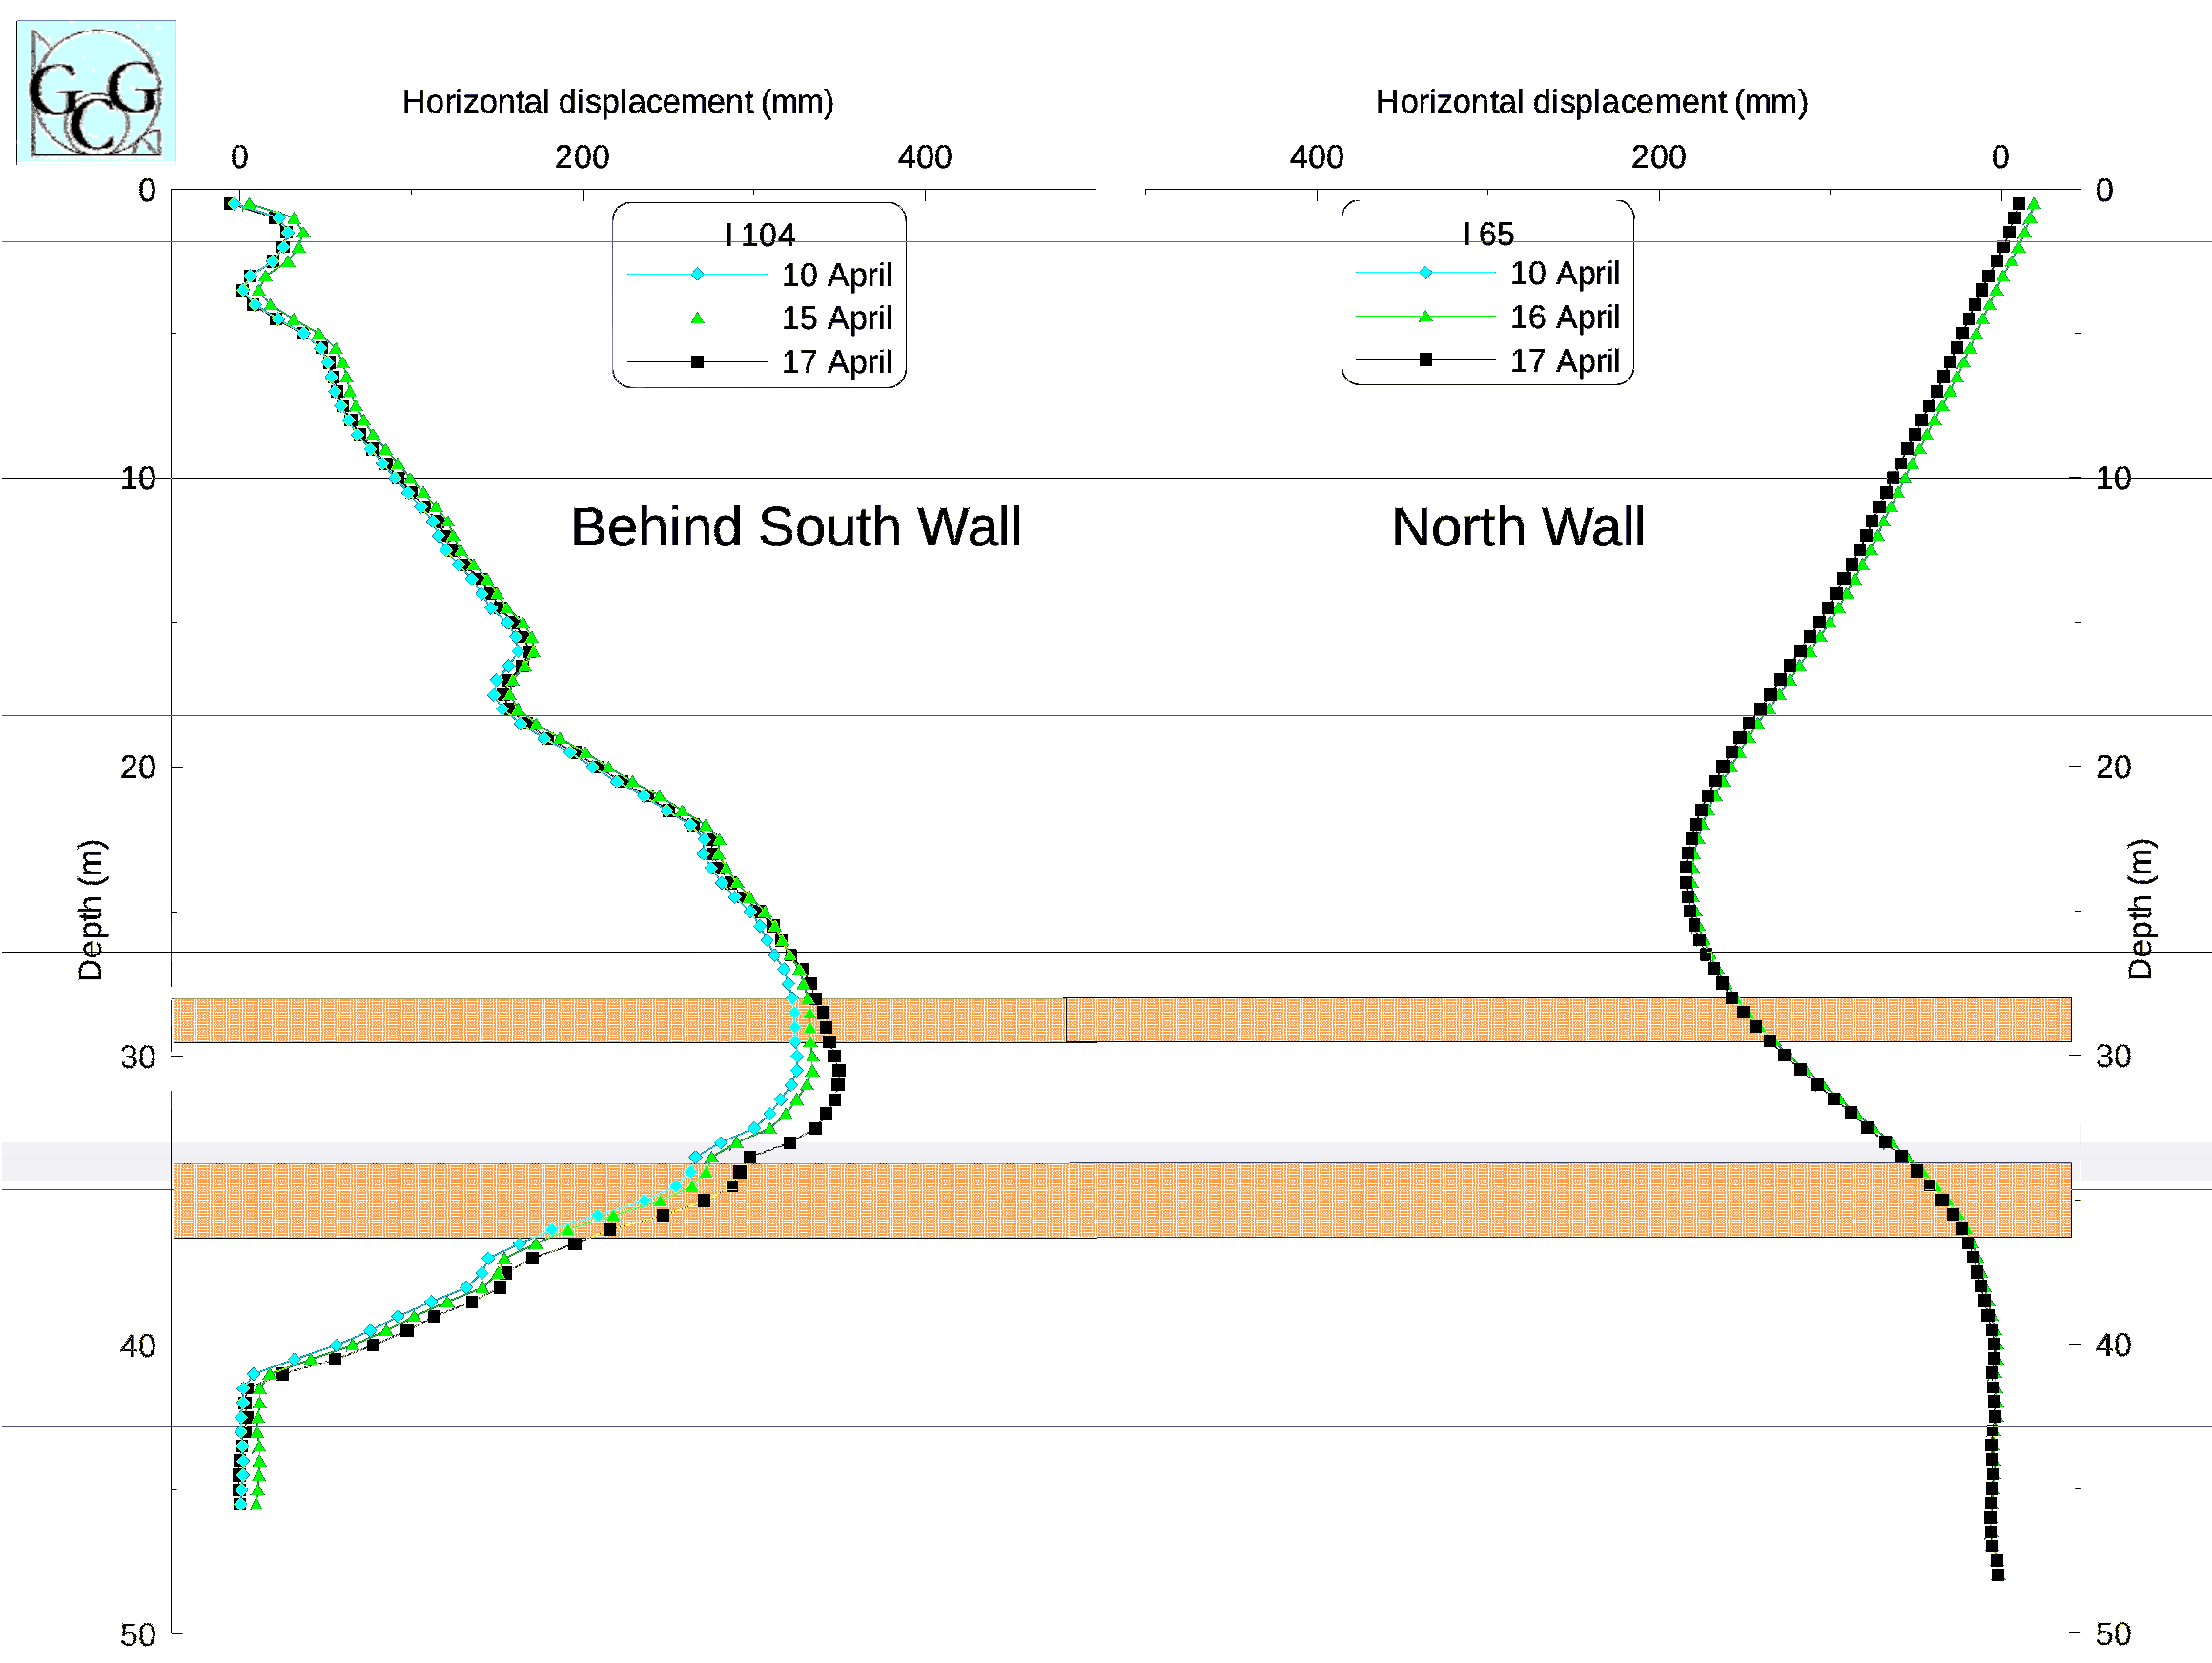
\includegraphics[width=0.8\textwidth]{figs/disp3.png}
\end{figure}
\end{frame}


%------------------------------------------------
\begin{frame}
\frametitle{Leading up to the collapse: Wall displacements}
\begin{figure}[ht]
	\centering
	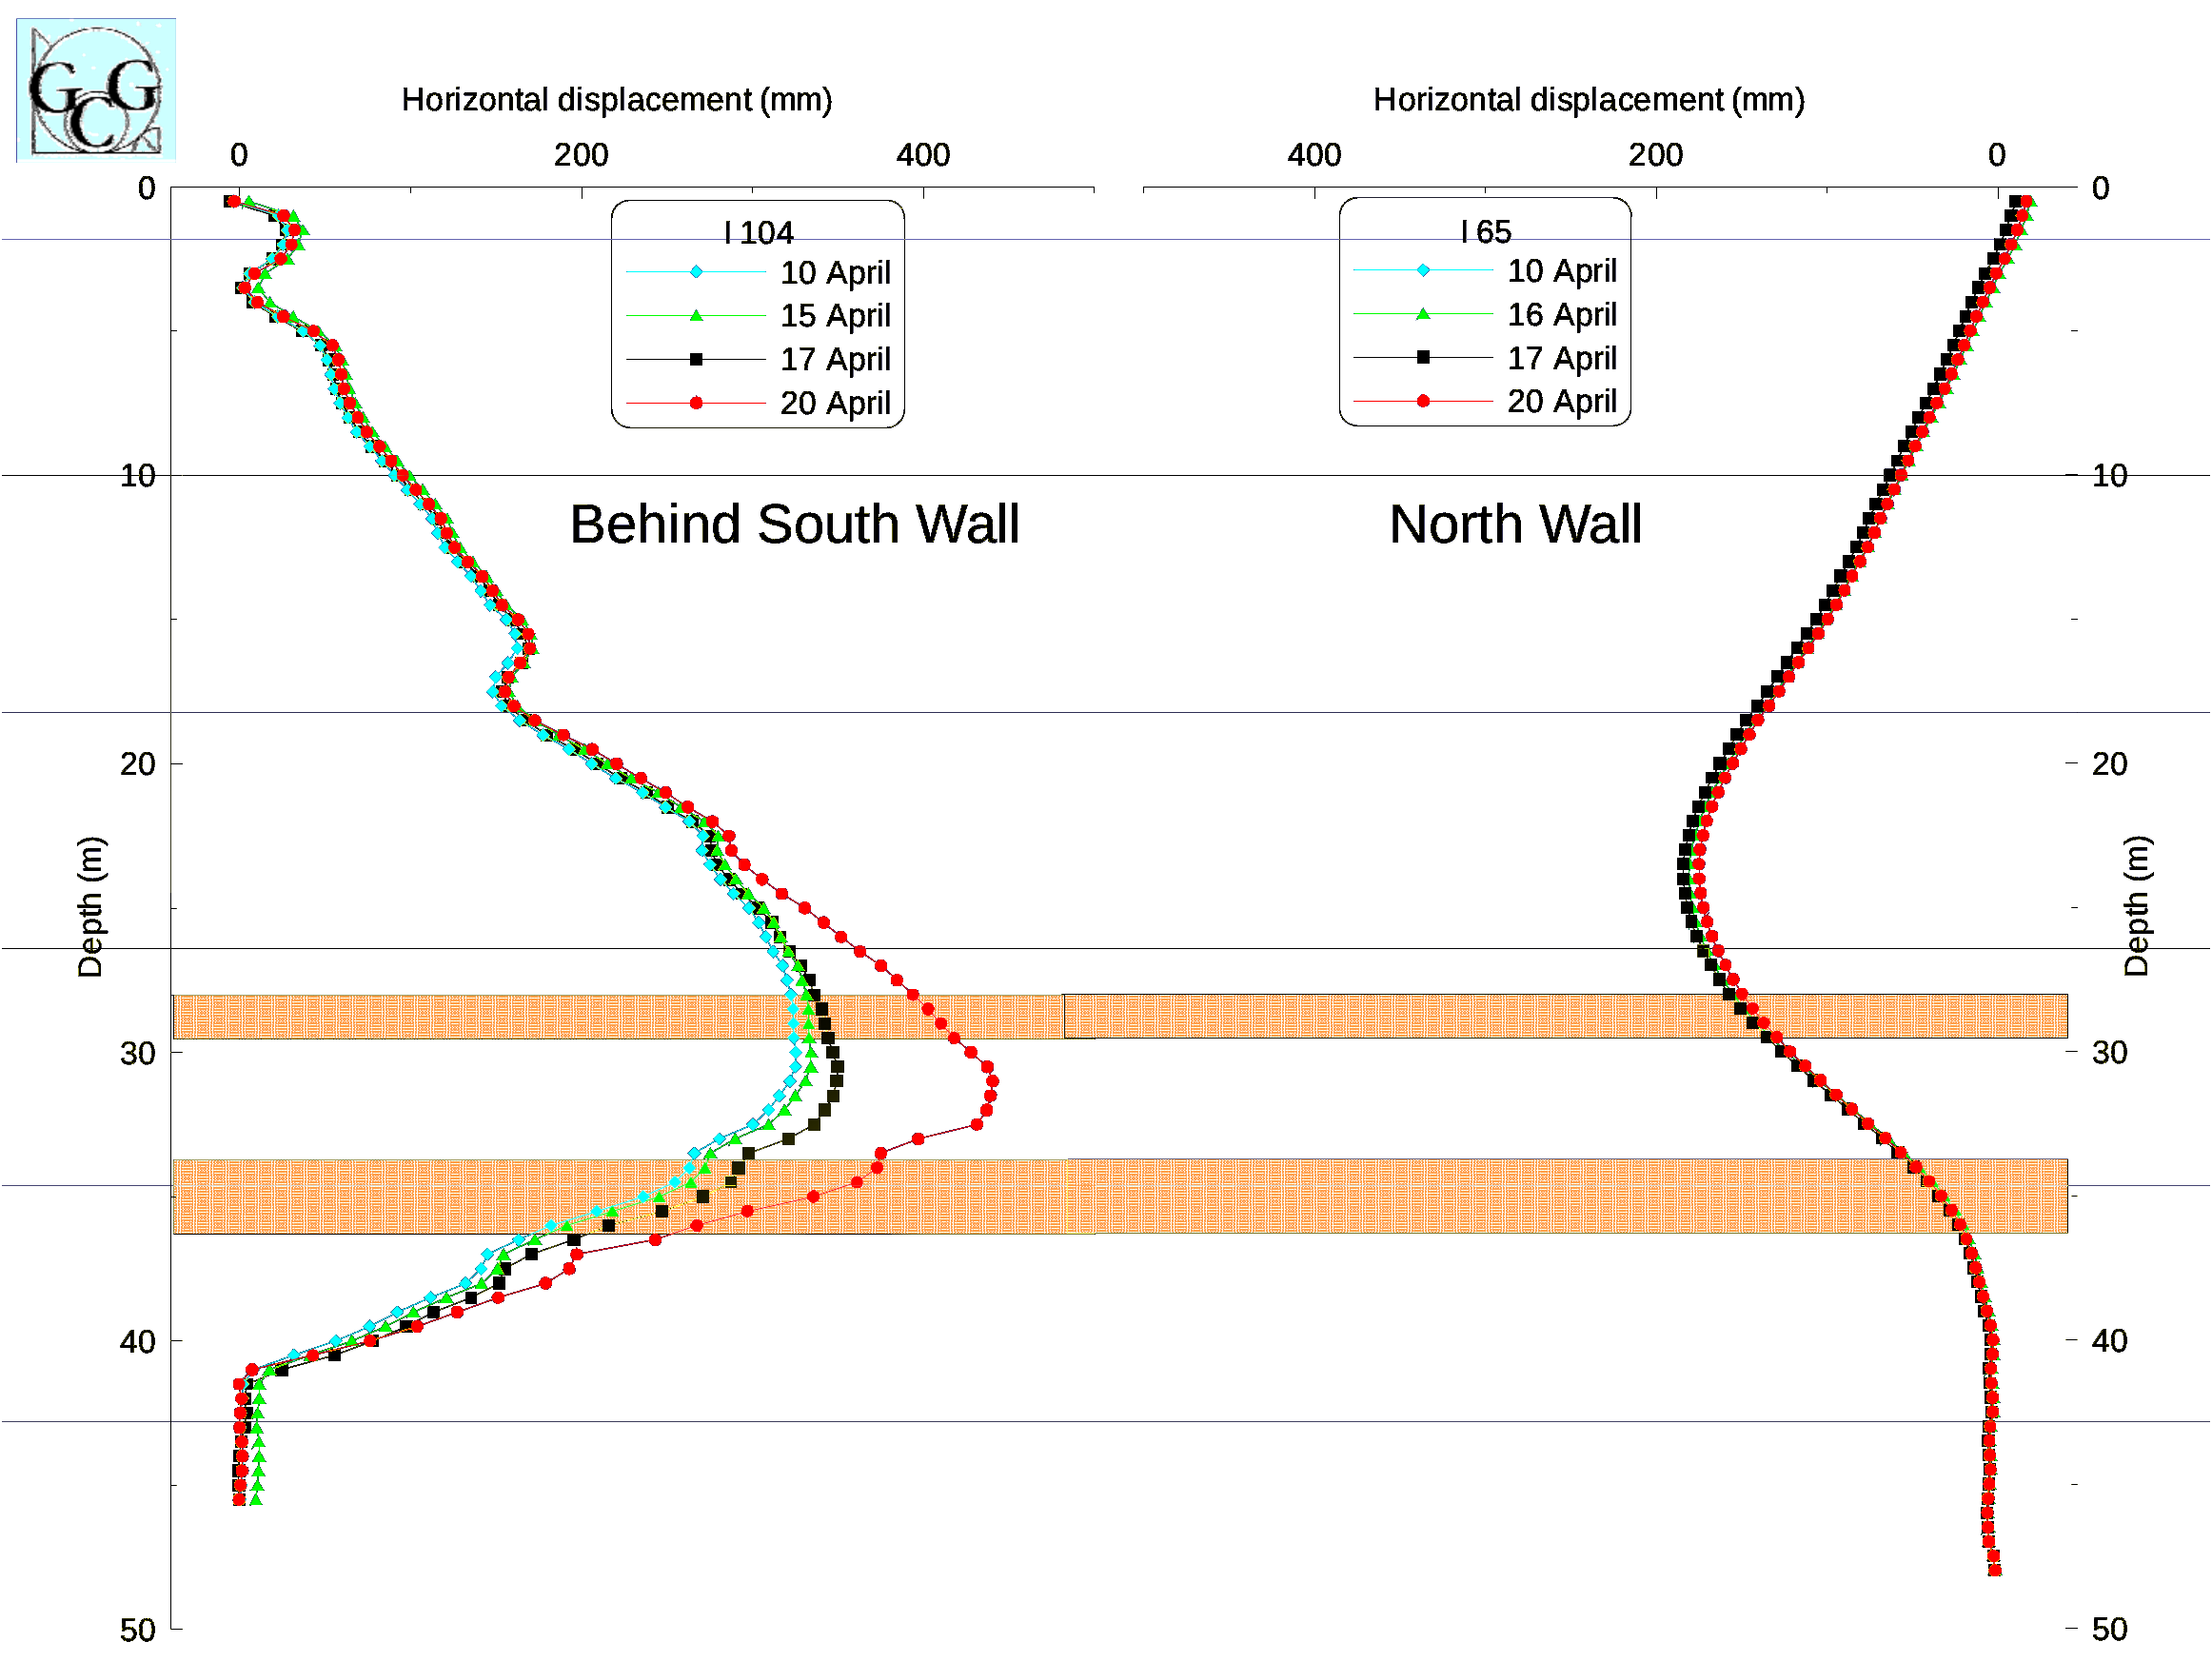
\includegraphics[width=0.8\textwidth]{figs/disp4.png}
\end{figure}
\end{frame}

\subsection{The Collapse}
%------------------------------------------------
\begin{frame}
\frametitle{The collapse}
\begin{figure}[ht]
	\centering
	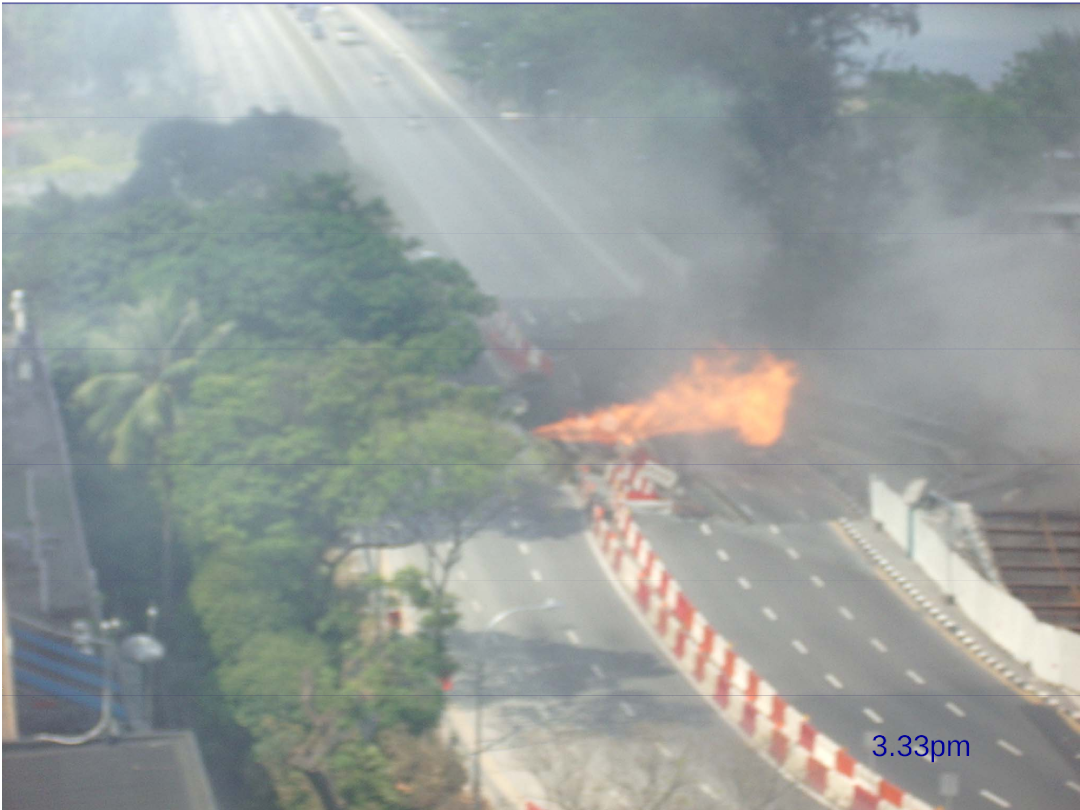
\includegraphics[width=0.85\textwidth]{figs/collapse1.png}
\end{figure}
\end{frame}

%------------------------------------------------
\begin{frame}
\frametitle{The collapse}
\begin{figure}[ht]
	\centering
	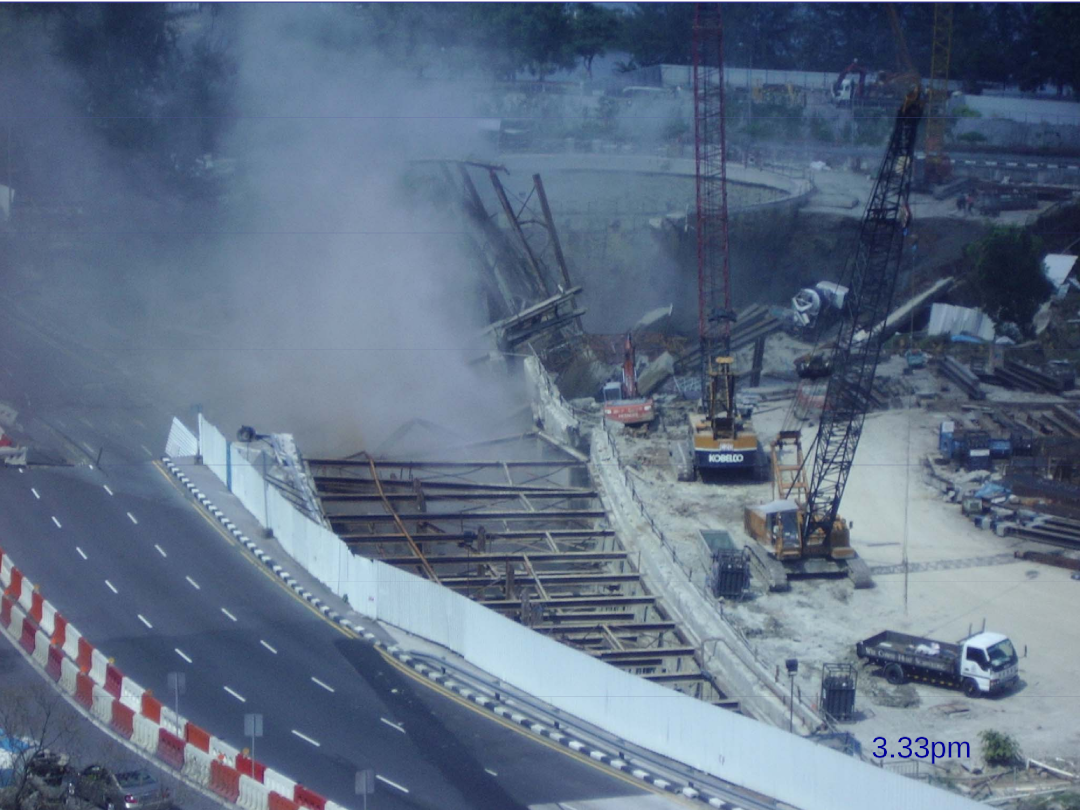
\includegraphics[width=0.85\textwidth]{figs/collapse2.png}
\end{figure}
\end{frame}

%------------------------------------------------
\begin{frame}
\frametitle{The collapse}
\begin{figure}[ht]
	\centering
	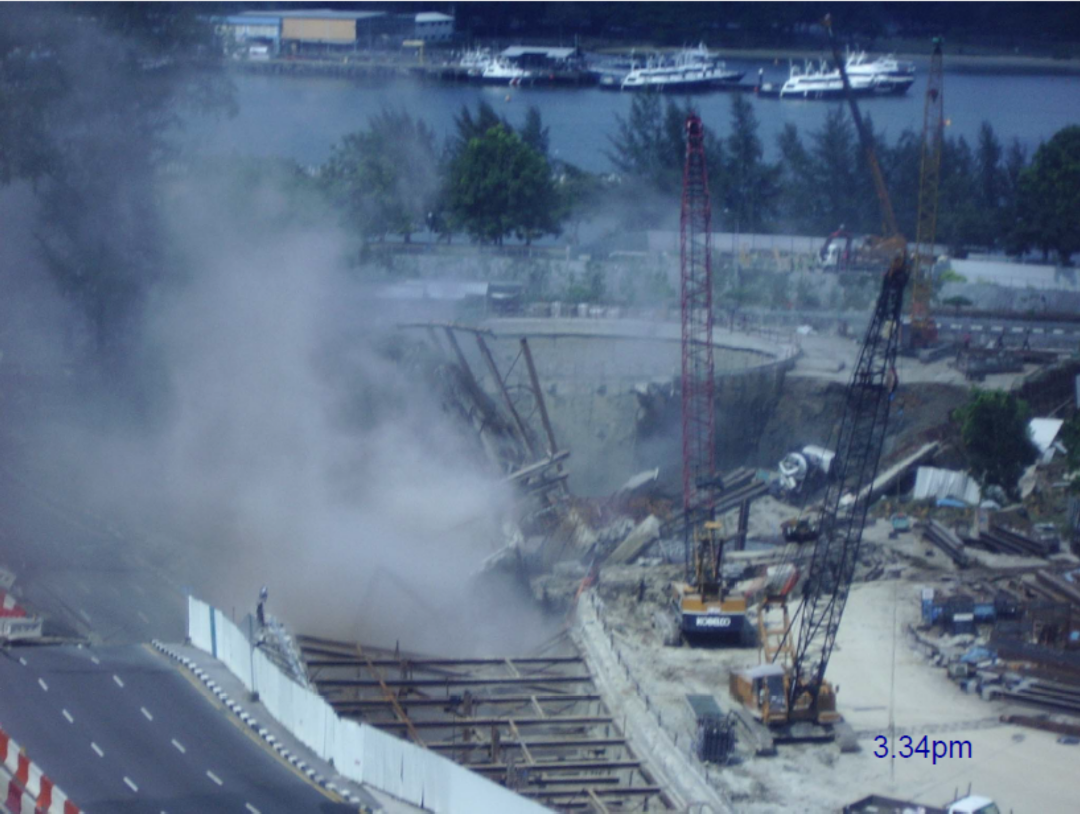
\includegraphics[width=0.85\textwidth]{figs/collapse3.png}
\end{figure}
\end{frame}

%------------------------------------------------
\begin{frame}
\frametitle{The collapse}
\begin{figure}[ht]
	\centering
	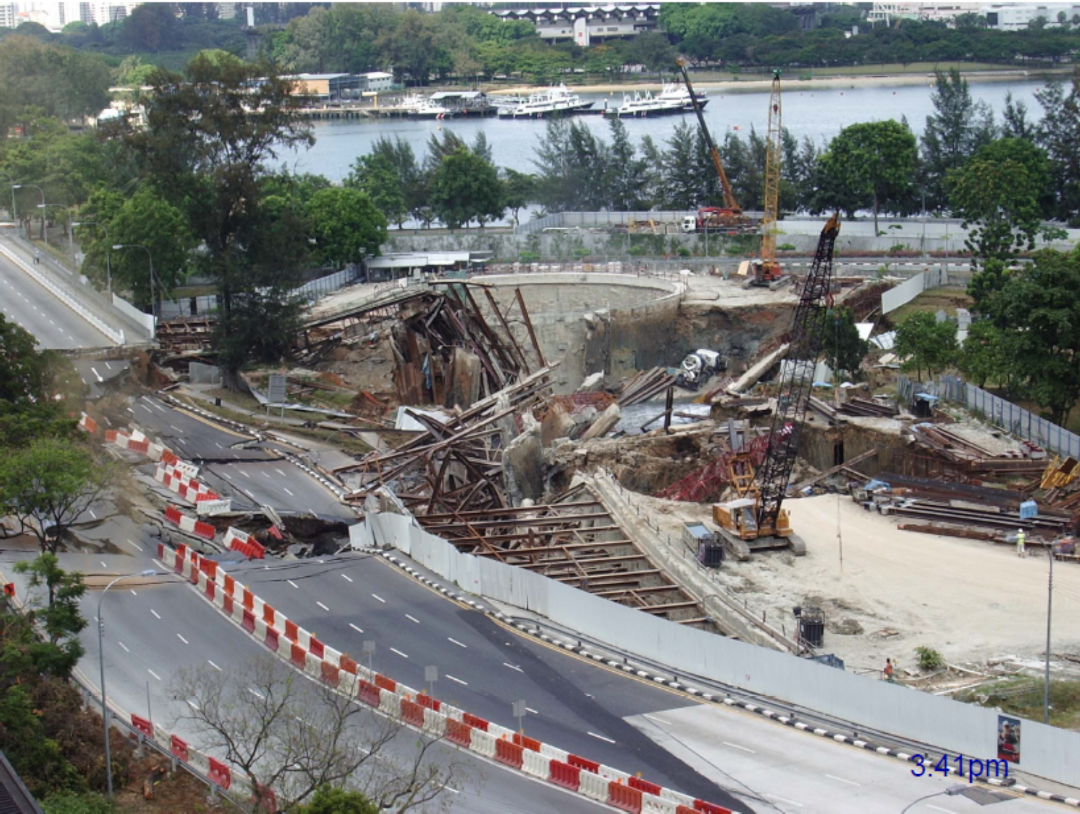
\includegraphics[width=0.85\textwidth]{figs/collapse4.png}
\end{figure}
\end{frame}

%------------------------------------------------
\begin{frame}
\frametitle{The collapse}
\begin{figure}[ht]
	\centering
	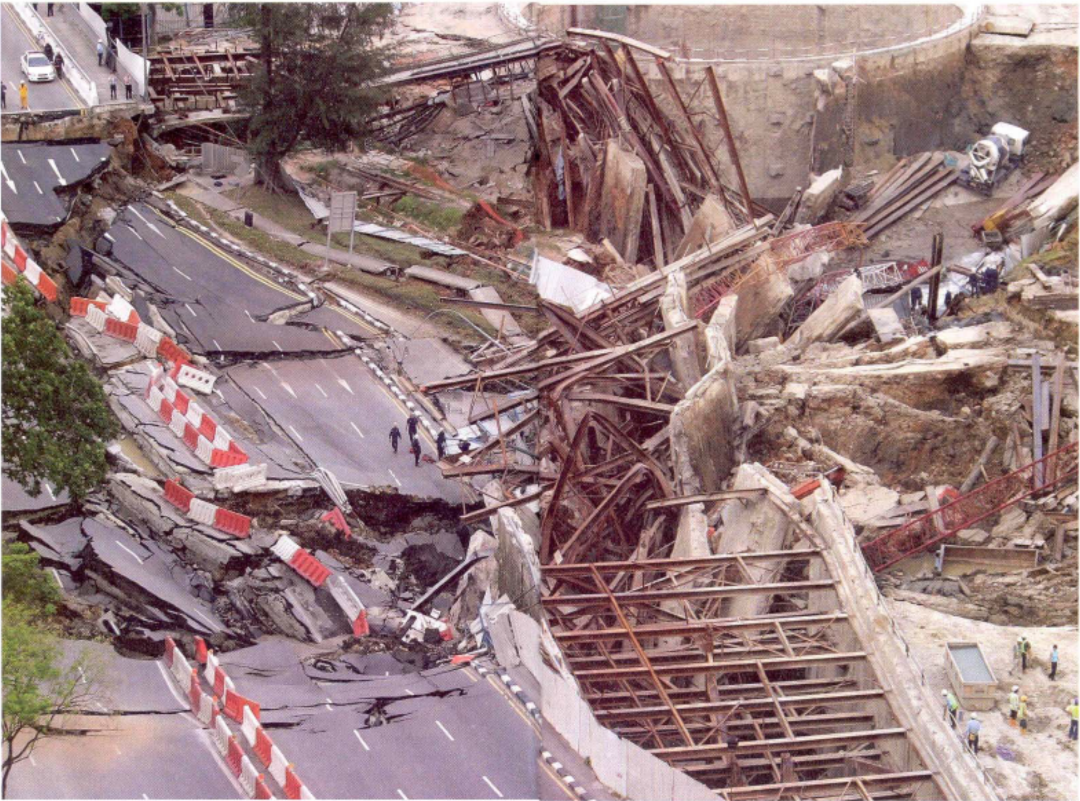
\includegraphics[width=0.85\textwidth]{figs/collapse5.png}
\end{figure}
\end{frame}

%------------------------------------------------
\begin{frame}
\frametitle{Post collapse}
\begin{figure}[ht]
	\centering
	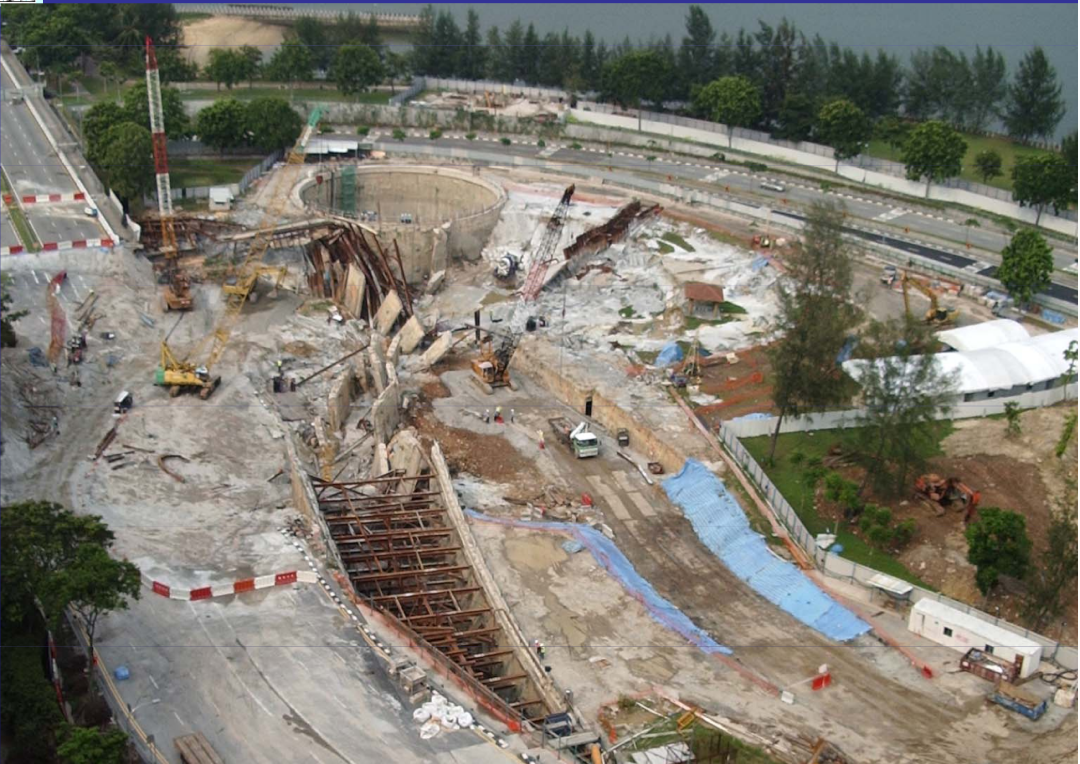
\includegraphics[width=0.85\textwidth]{figs/post-collapse.png}
\end{figure}
\end{frame}

%------------------------------------------------
\begin{frame}
\frametitle{Post collapse}
\begin{figure}[ht]
	\centering
	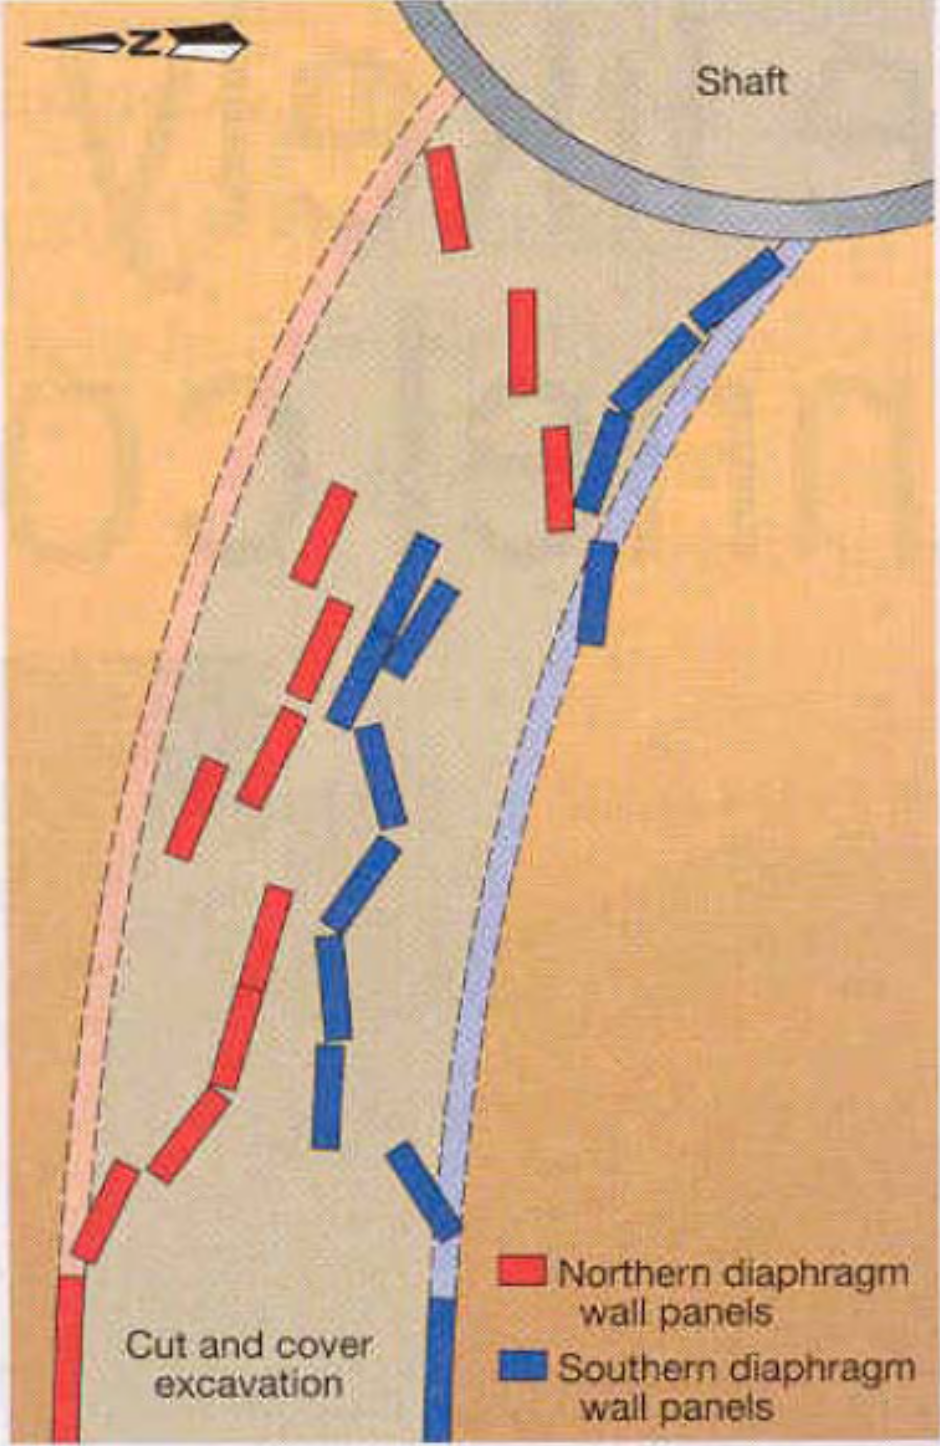
\includegraphics[width=0.4\textwidth]{figs/final-dwall-panels.png}
\end{figure}
\end{frame}

\subsection{Post collapse investigation}
%------------------------------------------------
\begin{frame}
\frametitle{Reasons for collapse}
\begin{figure}[ht]
	\centering
	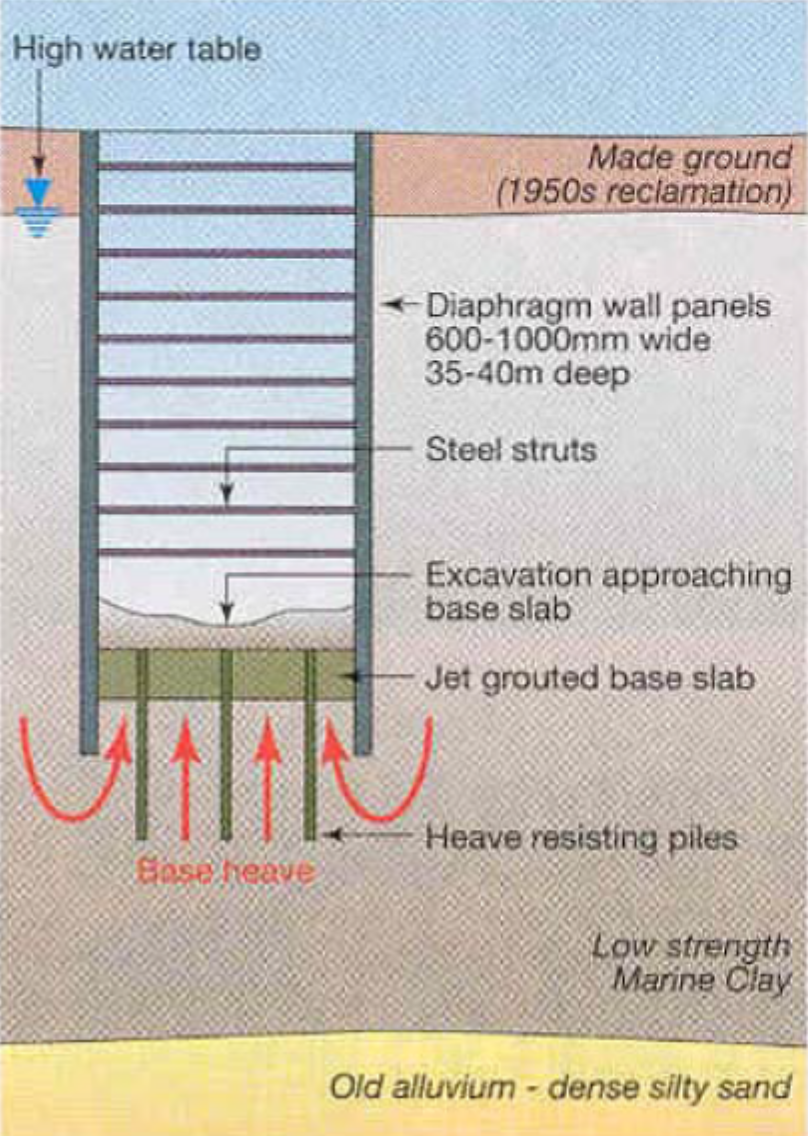
\includegraphics[width=0.45\textwidth]{figs/reasons-collapse.png}
\end{figure}
\end{frame}

\note{
	\begin{enumerate}
		\item Problem with jet grouting at the base of the slab.
		\item Struts design - connectors
		\item Use of effective stress parameters to do an undrained excavation.
	\end{enumerate}
}

%------------------------------------------------
\begin{frame}
\frametitle{Strut design: Replacing plate-stiffener with C-channel}
\begin{figure}[ht]
	\centering
	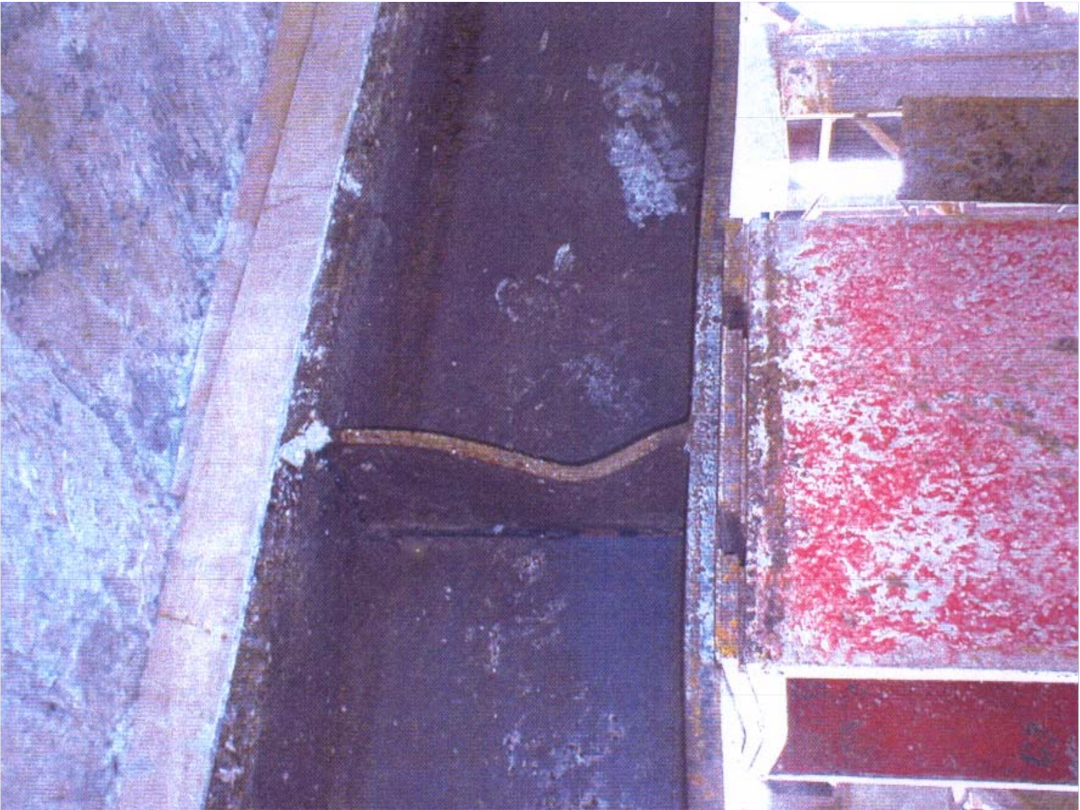
\includegraphics[width=0.85\textwidth]{figs/plate-stiffener.png}
\end{figure}
\end{frame}

%------------------------------------------------
\begin{frame}
\frametitle{Strut design: Waler connection}
\begin{figure}[ht]
	\centering
	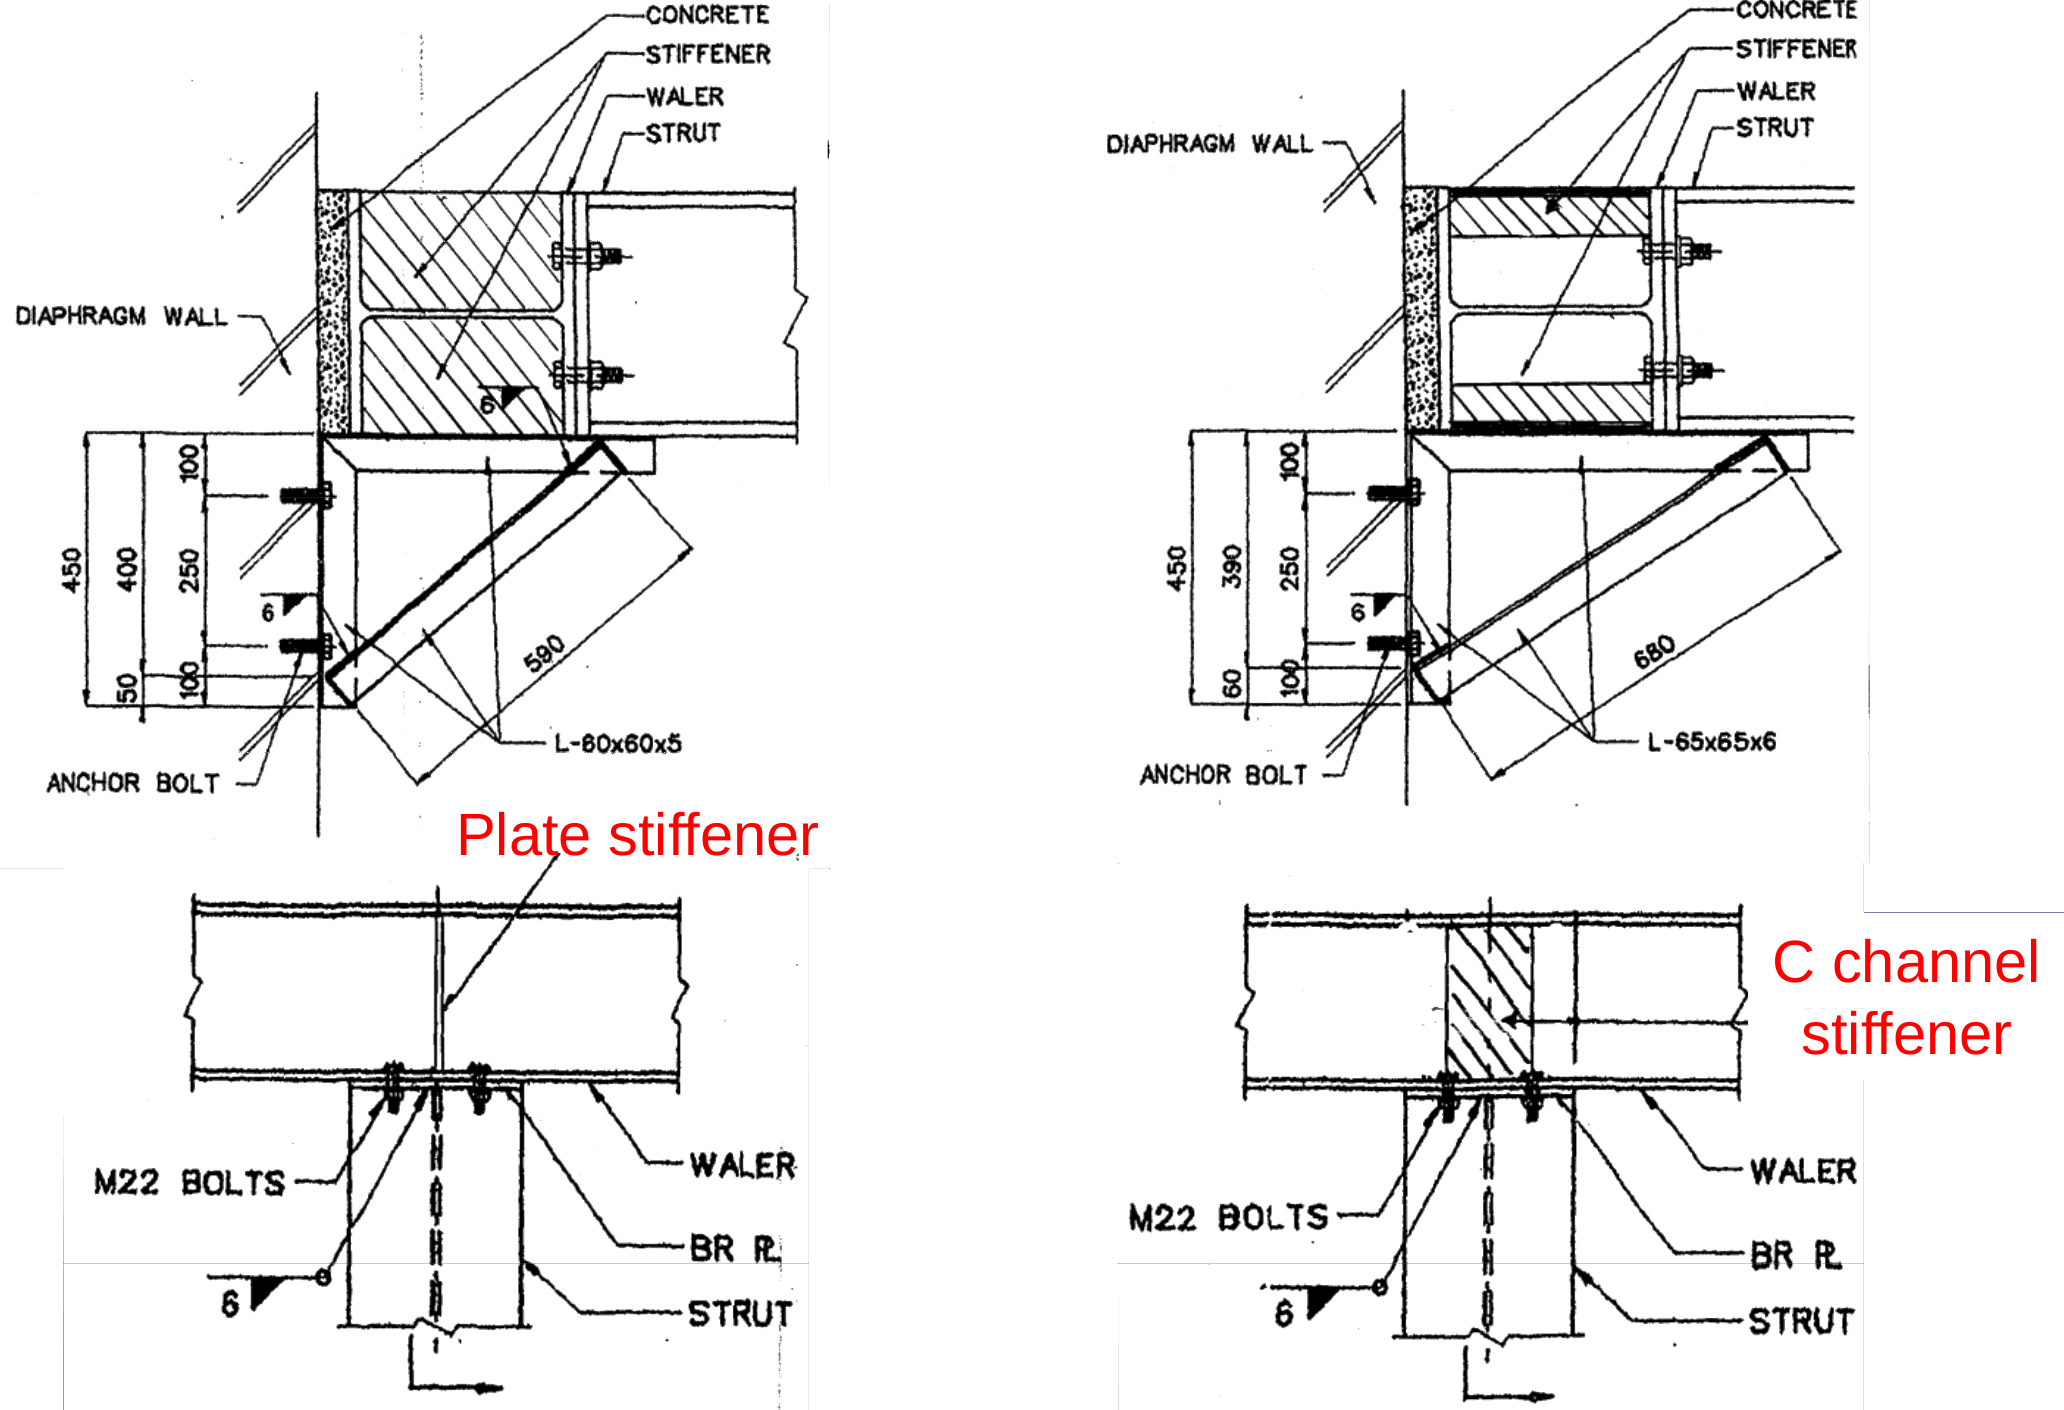
\includegraphics[width=0.85\textwidth]{figs/plate-stiffeners-strut-waler.png}
\end{figure}
\end{frame}

%------------------------------------------------
\begin{frame}
\frametitle{Strut design: Waler connection}
\begin{figure}[ht]
	\centering
	\includegraphics[width=0.85\textwidth]{figs/c-channel-strut-dwall.png}
\end{figure}
\end{frame}

%------------------------------------------------
\begin{frame}
\frametitle{Strut design: Waler connection}
\begin{figure}[ht]
	\centering
	\includegraphics[width=0.6\textwidth]{figs/waler-strut.png}
\end{figure}
\end{frame}

%------------------------------------------------

\note{
	Another chief reason for the failure was the under design of the waler-strut connection. Designers misinterpreted the \textbf{stiff bearing length for the C-channels as per BS 5950 to 400 mm instead of using 65 mm}. Waler connections with C-channels were designed with the effective length factor of 0.7, where the end conditions were unrestrained and a factor of 1.2 should have been used. This resulted in axial design capacity that was about 70\% of the assumed design load for the connection (COI 2005, pp 1-16). Also in some locations the splays in the waler strut connection had been omitted during construction (NCE, 2005). These design and construction errors resulted in the failure of the 9th level strut-waler system. The under designed diaphragm wall could not resist the redistributed loads as the 9th level strut-waler system failed resulting in the collapse of the tunnel.
}

%------------------------------------------------
\begin{frame}
\frametitle{Strut design: Relative vertical displacements}
\begin{figure}[ht]
	\centering
	\includegraphics[width=0.85\textwidth]{figs/relative-vertical-displacement.png}
	\caption*{Relative vertical displacement between the King Post and the Dwall}
\end{figure}
\end{frame}

%------------------------------------------------
\begin{frame}
\frametitle{Strut design: C-channel}
\begin{figure}[ht]
	\centering
	\includegraphics[width=0.85\textwidth]{figs/c-channel-stiffened.png}
\end{figure}
\end{frame}

%------------------------------------------------
\begin{frame}
\frametitle{Strut design: C-channel relative vertical displacement}
\begin{figure}[ht]
	\centering
	\includegraphics[width=0.85\textwidth]{figs/c-channel-effect-relative-vertical-disp.png}
\end{figure}
\end{frame}

%------------------------------------------------
\begin{frame}
\frametitle{Excavation of sacrificial jet grout}
\begin{figure}[ht]
	\centering
	\includegraphics[width=0.85\textwidth]{figs/excavation-jet-grout.png}
\end{figure}
\end{frame}

%------------------------------------------------
\begin{frame}
\frametitle{Quality of jet grouting}
\begin{figure}[ht]
	\centering
	\includegraphics[width=0.65\textwidth]{figs/jet-grout-cores.png}
\end{figure}
\end{frame}


%------------------------------------------------
\begin{frame}
\frametitle{Porepressure analysis in geotechnical engineering}
\mode<beamer>{
\begin{figure}[ht]
	\centering
	\includegraphics[width=\textwidth]{figs/geotechnical-analysis.png}
\end{figure}
}
\mode<handout>{
	\vspace{6cm}
}
\end{frame}


%------------------------------------------------
\begin{frame}
\frametitle{Undrained analysis}
\mode<beamer>{
	\begin{itemize}
		\item Method A and Method B refers to 2 alternatives modeling of undrained behaviour in Plaxis. 
		\item \textbf{Method A is an effective stress analysis} of an undrained problem it assumes an isotropic elastic behavior and a Mohr-Coulomb failure criterion. 
		\item As a result mean effective stress $p^\prime$ is constant until yield.
		\item Method A was being applied to marine clays which were of low over-consolidation or even under-consolidated because of recent reclamation.
	\end{itemize}
}
\mode<handout>{
	\vspace{6cm}
}
\end{frame}

%------------------------------------------------
\begin{frame}
\frametitle{Undrained effective stress analysis}
\mode<beamer>{
	\begin{figure}[ht]
		\centering
		\includegraphics[width=0.75\textwidth]{figs/mc_undrained}
	\end{figure}
}
\mode<handout>{
	\vspace{6cm}
}
\end{frame}

\note{
\textbf{Discuss the effect of depth on the increase in shear strength}
	\begin{figure}
		\includegraphics[width=0.6\textwidth]{figs/cu-method-a-b.png}
	\end{figure}
}
%------------------------------------------------
\begin{frame}
\frametitle{Wall displacements: Effective stress vs Undrained strength}
\begin{figure}[ht]
	\centering
	\includegraphics[width=\textwidth]{figs/wall-disp.png}
	\caption*{Method A vs Method B}
\end{figure}
\end{frame}

%------------------------------------------------
\begin{frame}
\frametitle{Bending moments: Effective stress vs Undrained strength}
	\begin{figure}[ht]
		\centering
		\includegraphics[width=\textwidth]{figs/bending-moments.png}
		\caption*{Method A vs Method B}
	\end{figure}
\end{frame}

%------------------------------------------------
\begin{frame}
\frametitle{Undrained effective stress analysis}
	\begin{itemize}
		\item 	Method A over-estimates the undrained shear
		strength of normally and lightly overconsolidated
		clays
		
		\item Its use led to a 50\% under-estimate of wall
		displacements and of bending moments and an
		under-estimate of the 9 th level strut force of 10\%
		
		\item The larger than predicted displacements mobilised
		the capacity of the JGP layers at an earlier stage
		than predicted
	\end{itemize}
\end{frame}

\note{
One of the major incidents that happened prior to the collapse was in the tunnel launch shaft area in August 2003. Tunnel launch shaft was located at the eastern end of the cut and cover tunnels. During the excavation of the tunnel launch shaft at about the 7th level of struts severe deflections of the diaphragm walls was observed which exceeded the design limit. Excessive ground settlement in the order of 400 mm was observed in a stadium nearby the south diaphragm wall (COI 2005, pp 36-54). Vertical cracks in some of the diaphragm wall panels were observed. Further excavation of the tunnel launch shaft was stopped immediately.}

\note{A back analysis was performed for the diaphragm walls based on effective stress approach and it was determined that the walls were not capable of withstanding the load if the excavation had proceeded. So the contractor constructed a jet grout pile layer and temporary walls to support the deflected wall and added additional struts to support the excavation before the excavation was resumed.

The critical error of using the effective stress approach in place of total stress approach overestimates the undrained shear strength of the marine clays which results in underestimation of the deflection, bending moment in the walls. This explanation was pointed out by the engineering advisory panel of the owners. They strongly suggested the contractors to reanalyze using the total stress approach. The contractor declined to reanalyze claiming that their design was sound and the fact that the excavation in other areas based on the effective stress approach behaved as designed. They eventually agreed to do a back analysis based on the TSA.}

\note{The contractors were reluctant to use the total stress approach for back analysis as they felt that the method gave large wall deflections, which would result in thicker walls. They also justified the use of effective stress approach based on the fact that the analysis provided similar results as the actual deflection of the walls. However this was partially true as for smaller depths the effective stress method would give close displacement results but as the excavation in the marine clay progresses the deflections calculated become highly un-conservative and wouldn’t match the actual deflection and so was still a very unsafe basis for design. Although this was not very clear at that point of time so the owners agreed to the further excavation of the various tunnel sections. }

\note{The critical error of using effective stress method for analysis and subsequent back analysis became more evident as the excavation progressed deeper. As the excavation of different sections of the tunnel were carried out in parallel, the excavation didn’t reach to such levels were the diaphragm walls would have failed. But the tunnel section near the Nicoll highway had to be excavated quicker than other sections as the construction and excavation work hindered with the traffic flow on the highway.}

\note{As the excavation of the M3 type walls progressed to about the 6th level of strut the deflection of the walls exceeded the design limit in February of 2004. The section was back analyzed using effective stress approach and the design limits were revised. The excavation progressed with the new revised deflection limits. By the end of March of 2004 the deflection of the walls had exceeded the revised deflection limits. A second back analysis was done based on the same effective stress method and the design deflection limits were further revised and remediation measures were taken to keep the excavation open. The owners accepted the second back analysis and permitted the further excavation on 3rd April 2004. Between 3rd April and the 20th April there were periods of time when the inclinometer readings were not monitored by the contractor.}

\end{document}